\documentclass[a4paper,oneside,12pt,fleqn]{article}
\usepackage[slovene]{babel}
\usepackage[utf8]{inputenc}
\usepackage[T1]{fontenc}
\usepackage{url}
\usepackage{graphicx}
\usepackage{epstopdf}
\usepackage[usenames]{color}
\usepackage[reqno]{amsmath}
\usepackage{amssymb}
\usepackage{icomma}
\usepackage[bookmarks, colorlinks=true, unicode=true,%
linkcolor=black, anchorcolor=black, citecolor=black, filecolor=black,%
menucolor=black, runcolor=black, urlcolor=black%
]{hyperref}
\hypersetup{pdftitle={Teorija pri matematiki}}
\hypersetup{pdfauthor={Jure Slak}}
\hypersetup{pdfsubject={Zapiski}}
\usepackage[
    paper=a4paper,
    top=2.5cm,
    bottom=2.5cm,
%    textheight=24cm,
    textwidth=15cm,
    ]{geometry}

\usepackage{amsthm}
{
\newtheorem{izrek}{Izrek} %[section]
\newtheorem{dokaz}[izrek]{Dokaz}
\newtheorem{trditev}[izrek]{Trditev}
\newtheorem{posledica}[izrek]{Posledica}
{
\theoremstyle{definition}
\newtheorem{definicija}{Definicija}
}
}

%\usepackage{makeidx} % stvarno kazalo
%\makeindex

\usepackage{enumerate} % za lep enumerate
\usepackage{auto-pst-pdf} % slike
\usepackage{pst-plot} %slike
\usepackage{pst-math} %slike 
\usepackage{pst-eucl} %slike 
\usepackage{subfigure} % podlsike
%\usepackage{multido} % while
\usepackage{gensymb} % stopinje
\usepackage{tabularx} % stretching table
\usepackage{pbox} % multi line table cell
\usepackage{units} % da lahko napišeš 12kg lepo v math modu
\usepackage{mathtools} % matrike z alignment specification
\usepackage{footmisc} % da lahko ponavlam footnote
\usepackage{floatflt} % floating figure and table
\usepackage{algorithm} % za algoritem kot float
\usepackage{algpseudocode} % za psevdokodo 

\def\R{\ensuremath{\mathbb R}}
\def\N{\ensuremath{\mathbb N}}
\def\Z{\ensuremath{\mathbb Z}}
\def\C{\ensuremath{\mathbb C}}
\def\Q{\ensuremath{\mathbb Q}}
\def\I{\ensuremath{\mathcal I}}
\mathchardef\mhyphen="2D

\newcommand{\edot}{\;\;\;.}
\newcommand\krat\cdot
\newcommand{\Rel}{\mathcal{R}}
\newcommand{\comment}[1]{\ensuremath{\qquad\backslash\backslash\;}\textnormal{#1}}

\makeatletter
\newcommand{\rom}[1]{\romannumeral #1}
\newcommand{\Rom}[1]{\expandafter\@slowromancap\romannumeral #1@}
\makeatother

\makeatletter
\newcommand{\hyperanchor}[1]{\Hy@raisedlink{\hypertarget{#1}{}}}
\makeatother

% operators
\newcommand{\beforecaptionskip}{\vspace{-12pt}}
\newcommand{\arccot}{\ensuremath{\operatorname{arccot}}} % arccot
\newcommand{\tg}{\ensuremath{\operatorname{tg}}} % tg 
\newcommand{\ctg}{\ensuremath{\operatorname{ctg}}} % ctg
\newcommand{\pr}{\ensuremath{\operatorname{pr}}} % pravokotna projekcija
\newcommand{\st}{\ensuremath{\operatorname{st}}} % stopnja polinoma

% PST DRAWING
% colour settings
\newrgbcolor{lightgreen1}{0.3164 0.9531 0.3125}
\newrgbcolor{lightgrey}{0.8 0.8 0.8}
\newrgbcolor{verylightgrey}{0.9 0.9 0.9}
\newrgbcolor{skyblue}{0.3125 0.5898 0.9531}
\newrgbcolor{orange}{0.9531 0.5625 0.3125}
\newrgbcolor{violet}{0.6172 0.3125 0.9531}
\newrgbcolor{pink}{0.9258 0.3125 0.9531}
\newrgbcolor{lightred}{0.9531 0.3125 0.3867}
\newrgbcolor{lightorange}{0.9531 0.7031 0.3125}
\newrgbcolor{lightgreen2}{0.5547 0.9141 0.2734}
\psset{arrowscale=1.5,RightAngleSize=.3} % arrow settings, angle markers


\newcommand{\asimptota}{\psline[linecolor=lightgrey, linestyle=dashed, linewidth=.5pt]}
\newcommand{\oznaka}{\psline[linecolor=red, linestyle=dotted]}
\newcommand{\ii}{\ensuremath{\imath}}
\def\kos{\cos}
\def\deg{\degree}
\def\Vec{\overrightarrow}
\def\konj{\overline} % conjugate
\def\limi{\displaystyle\lim_{n\to\infty}} % limit to infty
\def\limh{\lim_{h\rightarrow0}} % limit h to 0
\def\sumi{\displaystyle\sum^{\infty}} % sum to infty
\renewcommand{\d}{\ensuremath{\,d}} %use mathrm{d} for non italic d
\newcommand{\dx}{\ensuremath{\d x}}
\newcommand{\df}{\ensuremath{\d f}}
\newcommand{\dt}{\ensuremath{\d t}}
\newcommand{\du}{\ensuremath{\d u}}
\newcommand{\dv}{\ensuremath{\d v}}

\allowdisplaybreaks[1] % prelomi align

% multi line table cell with 0.5mm margin
\newcommand{\mltc}[1]{\pbox{21cm}{\vspace{0.5mm} #1 \vspace{0.5mm}}}
% new column type that expands and centers content
\newcolumntype{C}{>{\centering\arraybackslash}X}

% your definitions here ... 

% arrow resetings
\renewcommand\implies\Rightarrow
\renewcommand\iff\Leftrightarrow

%counter settings
\numberwithin{equation}{section}
\setcounter{lofdepth}{2}

\title{Teorija pri matematiki}
\author{Jure Slak}
\date{\today}

% space settings
\setlength{\parindent}{0pt}
\setlength{\parskip}{5pt}

\newenvironment{itemize*}%
{
\vspace{-12pt}%
\begin{itemize}%
\setlength{\itemsep}{0pt}%
\setlength{\parskip}{2pt}}%
{\end{itemize}}

\newenvironment{enumerate*}%
{
\vspace{-12pt}%
\begin{enumerate}%
\setlength{\itemsep}{0pt}%
\setlength{\parskip}{2pt}}%
{\end{enumerate}}

\newenvironment{description*}%
{
\vspace{-12pt}%
\begin{description}%
\setlength{\itemsep}{0pt}%
\setlength{\parskip}{2pt}}%
{\end{description}}

% aligned list
\newenvironment{xlist}[1][\rule{0.75 cm}{0cm}]{%
\vspace{-14pt}
  \begin{list}{}{%
    \settowidth{\labelwidth}{#1:}
    \setlength{\labelsep}{0.5cm}
    \setlength{\leftmargin}{\labelwidth}
    \addtolength{\leftmargin}{\labelsep}
    \addtolength{\leftmargin}{20pt}
    \setlength{\rightmargin}{0pt}
    \setlength{\parsep}{0.5ex plus 0.2ex minus 0.1ex}
    \setlength{\itemsep}{0 ex plus 0.2ex}
    \renewcommand{\makelabel}[1]{##1:\hfil}
    }
  }
{\end{list}}

% fixind description and list labels (using hyperref}
\makeatletter
\let\orgdescriptionlabel\descriptionlabel
\renewcommand*{\descriptionlabel}[1]{%
\let\orglabel\label
\let\label\@gobble
\phantomsection
\edef\@currentlabel{#1}%
\let\label\orglabel
\orgdescriptionlabel{#1}%
}
\makeatother

\begin{document}
%set spacing 2
\setlength{\abovedisplayskip}{3pt}
\setlength{\belowdisplayskip}{6pt}

\renewcommand{\listfigurename}{Kazalo slik} 
\floatname{algorithm}{Algoritem}

\thispagestyle{empty}
% naslovnica

\mbox{}\\
\vspace{3ex}

\noindent \scalebox{1.8}[2.1]{\textsf{{\Huge \bfseries Teorija pri}}} \\[5pt]
\scalebox{1.8}[2.1]{\textsf{{\Huge \bfseries matematiki}}} \\[60pt]
\scalebox{1}[1.2]{\textsf{\Huge \bfseries Jure Slak}} \\[45pt]
\textsf{2008 -- 2012, Gimnazija Vič}

\vspace{-10pt}
\noindent \mbox{} \hspace{-20pt} \scalebox{35}{$e^{\pi i}$}

\vfill
\hfill
\vspace{-5ex}
\scalebox{0.7}{v. 0.98}
%\vfill
%\hfill 

\pagebreak

\thispagestyle{empty}
\tableofcontents
\pagebreak

\section{Izjave}
\label{sec:izjave}
\textbf{Izjava} je smiseln povedni stavek, ki mu lahko določimo njegovo vrednost.

\textbf{Negacija} izjave $A$ je nova izjava, ``Ni res, da drži $A$.'' ($\neg A$), ki je pravilna, če je izjava $A$
napačna in obratno. 

\textbf{Konjunkcija} izjav $A$ in $B$ je nova izjava ``$A$ in $B$.'' ($A \land
B$), ki je pravilna le, če sta izjavi $A$ in $B$ pravilni.

\textbf{Disjunkcija} izjav $A$ in $B$ je nova izjava ``$A$ ali $B$.'' ($A \lor B$), 
ki je pravilna, ko je pravilna vsaj ena izmed izjav $A$ in $B$.

\textbf{Implikacija} izjav $A$ in $B$ je nova izjava ``Če $A$, potem sledi $B$.'' ($A
\implies B$), ki je napačna samo v primeru, da je prva izjava pravilna, druga pa napačna.

\textbf{Ekvivalenca} izjav $A$ in $B$ je nova izjava ``Če $A$, natanko takrat $B$.'' ($A 
\iff B$), ki je pravilna, če imata izjavi enako vrednost.

\section{Množice}
\label{sec:mnozice}
\textbf{Množica} je skupina elementov, ki jih druži neka skupna lastnost. 

\textbf{Prazna množica} je množica brez elementa. ($\emptyset$)

\textbf{Univerzalna množica} ($\mathcal{U}$) je množica, ki vsebuje vse elemente, ki jih preučujemo.

Množica $A$ je \textbf{podmnožica} $B$ ($A \subset B$), če je vsak element množice $A$ tudi element
množice $B$.

Dve množici sta \textbf{enaki}, če imata iste elemente.

\textbf{Moč} množice je število njenih elementov. ($\text{m}(a) \text{ ali } |A|$) 

\textbf{Unija} množic $A$ in $B$ ($A \cup B$) je nova množica, ki vsebuje elemente, ki so v množici $A$ ali v
množici $B$. \[ A \cup B = \left\{x:x \in A \lor x \in B \right\}, \quad \min\{|A|, |B|\} \le |A \cup B| \le |A| + |B| \]

\textbf{Presek} množic $A$ in $B$ ($A \cap B$) je nova množica, ki vsebuje elemente, ki so v množici $A$ in v
množici $B$. \[ A \cap B = \left\{x:x \in A \land x \in B \right\}, \quad 0 \le |A \cap B|
\le \min\{|A|, |B|\} \]

\textbf{Razlika} množic $A$ in $B$ ($A - B$ ali $A \setminus B$) je nova množica, ki
vsebuje vse elemente, ki so v prvi množici v prvi pa ne. 
\[ A - B = \left\{x : x \in A; x \notin B \right\} \]

\textbf{Komplement} množice $A$ ($A^c$) je nova množica, ki vsebuje vse elemente, ki niso
v množici $A$. $A^c = \mathcal{U} - A$

\textbf{Potenčna množica} množice $A$ je množica vseh podmnožic množice $A$.
\[ |\mathcal{P}(A)| = 2^{|A|} \comment{Za dokaz glej razdelek~\ref{sec:komb:bin}.} \]

\textbf{Kartezični produkt} množic $A$ in $B$ ($A \times B$) je nova množica, ki vsebuje urejene pare, v katerih
je prvi element iz množice $A$, drugi pa iz množice $B$. 
\[ A \times B = \left\{ \left(a, b \right); a \in A \land b \in B \right\}, \; \left|A \times B \right| = \left|A\right|
\krat \left|B\right| \]

Množice lahko predstavimo z Vennovimi diagrami, kot na primer na
sliki~\ref{fig:mnoz:venn}, kartezični produkt pa kot šahovnico ali kot mrežo, kjer vodoravne črte
predstavljajo elemente množice $A$, navpične elemente množice $B$, presečišča pa so
elementi kartezičnega produkta. Taka predstavitev je prikazana na
sliki~\ref{fig:mnoz:kart}.

\begin{figure}[h]
  \begin{center}
    \subfigure[Predstavitev razlike množic $A$ in $B$ z Vennovim diagramom.]{
      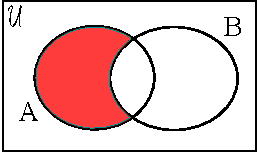
\includegraphics[width=0.4\textwidth]{slike/venn.pdf}
      \label{fig:mnoz:venn}
      }\hspace{2em}
    \subfigure[Predstavitev kartezičnega produkta $A \times B$.] {
      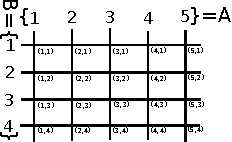
\includegraphics[width=0.4\textwidth]{slike/kart.pdf}
      \label{fig:mnoz:kart}
    }
  \end{center}
  \beforecaptionskip
  \caption{Grafična predstavitev množic.}
  \label{fig:mnoz}
\end{figure}

\section{Preslikave}
\label{sec:preslikave}
\textbf{Preslikava}, ki množico $A$ preslika v množico $B$ ($f\!\!: A \rightarrow B,
f\!\!:a \mapsto b$), je predpis, ki vsakemu elementu iz
množice $A$ priredi natanko določen element iz množice $B$. 

Preslikava je \textbf{injektivna}, kadar se par različnih elementov iz množice $A$ preslika v par
različnih elementov iz množice $B$. ($a_1 \neq a_2 \implies f(a_1) \neq f(a_2); a_1, a_2
\in A$)

Preslikava je \textbf{surjektivna}, kadar je vsak element množice $B$ slika vsaj enega elementa iz
množice $A$. ($\forall b \in B, \exists a \in A\!: b = f(a)$)

Preslikava je \textbf{bijektivna}, če je injektivna in surjektivna hkrati.

Graf preslikave $f\!\!: A \rightarrow B$ je podmnožica kartezičnega produkta $A \times B$.

\section{Relacije}
\label{sec:relacije}
\textbf{Relacija} je odnos med elementi neke množice.
Relacija je podmnožica kartezičnega produkta.

Relacija je \textbf{refleksivna}, če za vsak element v množici velja, da je element v relaciji sam s
seboj. ($\Rel \text{ refleksivna} \iff \forall a \in A\!: a \Rel a$)

Relacija je \textbf{simetrična}, kadar za vsak par elementov velja: če je prvi v relaciji z drugim,
je tudi drugi v relaciji s prvim. 
($\Rel \text{ simetrična} \iff \forall a, b \in A\!: a \Rel b \implies b \Rel a$)

Relacija je \textbf{tranzitivna}, če za vsako trojico elementov velja: če je prvi v relaciji z
drugim in drugi v relaciji s tretjim, potem je tudi prvi v relaciji s tretjim.
($\Rel \text{ tranzitivna} \iff \forall a, b, c \in A\!: (a \Rel b \land b \Rel c) \implies a \Rel c$)

Relacija je \textbf{ekvivalenčna}, če je refleksivna, simetrična in tranzitivna hkrati.

\section{Naravna števila}
\label{sec:naravna}
\[ \N = \left\{1, 2, 3, 4, 5, 6, \ldots \right\} \]
\[ \N_0 = \N \cup \left\{ 0 \right\} \]

Z $\N_n$ označimo množico prvih $n$ naravnih števil.

\textbf{Operacija} dvema elementoma priredi nov element.

Definirajmo še soda in liha števila: \\
$\mathcal S = \{2n; n \in \N \}$ \\
$\mathcal L = \{2n+1; n \in \N \}$

Velja tudi: \\
vsota dveh lihih števil je sodo število. 
\[ (2n+1) + (2m+1) = 2(n+m+1) = 2k \]
kvadrat lihega števila je liho število. 
\[ (2n+1)^2 = 4n^2 + 4n + 1 = 2(2n^2 + 2n) + 1 = 2k+1 \]

\subsection{Zakoni}
\label{sec:naravna:zakoni}
Zakon o \textbf{komutativnosti} ali zakon o zamenjavi za množenje in seštevanje:
\[ a + b =  b + a \]
\[ a \krat b =  b \krat a \]

Zakon o \textbf{asociativnosti} ali zakon o združevanju za množenje in seštevanje:
\[ a + (b + c) = (a + b) + c \]
\[ a \krat (b \krat c) = (a \krat b) \krat c \]

Zakon o \textbf{distributivnosti} ali zakon o razčlenjevanju, ki povezuje množenje in seštevanje:
\[ a \krat (b + c) = a \krat b + a \krat c \]

\subsection{Številski sestavi}
Vsako število v desetiškem sistemu z osnovo 10 lahko zapišemo v kateremkoli sistemu
z osnovo $b$. \\
Poljubno število $a_na_{n-1}\!\ldots a_2a_1a_0$ pomeni:
\[ a_n \krat b^n + a_{n-1} \krat b^{n-1} + \cdots + a_2 \krat b^2 +a_1 \krat b + a_0 \]

$b$ --- osnova, $b \in \N \land b \geq 2$ \\
$a_i$ --- števka, cifra, $0 \leq a_i < b$

Vsako naravno število $a$ lahko zapišemo na en sam način v številskem sestavu z osnovo $b$.

\subsection{Relacija deljivosti}
Število $a$ deli število $b$ natanko takrat, ko je število $b$ večkratnik števila $a$.
\[ a | b \iff b = k \krat a;\quad a, b, k \in \N \]

\textbf{Lastnosti:}
\begin{xlist}[Antisimetričnost]
  \item[refleksivnost]       $a|a$
  \item[antisimetričnost]  $a|b \land b|a \implies a = b$
  \item[tranzitivnost]      $a|b \land b|c \implies a|c$
  \item[neimenovana 1]      $a|b \land a|c \implies a|\left( b+c \right)$
  \item[neimenovana 2]      $a|b \land a|\left( b+c \right) \implies a|c$
\end{xlist}

\textbf{Dokaz antisimetričnosti:}
\begin{align}
  a|b \iff b &= k_1 \krat a; \quad k_1 \in \N \\
  b|a \iff a &= k_2 \krat b; \quad k_2 \in \N \label{eq:del:antis:akb} \\
  a &= k_2 \krat b \comment{izhaja iz definicije} \label{eq:del:antis:akb2} \\
  a &= k_2 \krat k_1 \krat a \comment{$b$ zamenjamo po definiciji, glej \eqref{eq:del:antis:akb}} \\
  k_1 \krat k_2 &= 1 \\
  k_1 &= 1, k_2 = 1 \label{eq:del:antis:kk} \comment{$k_1k_2$ je lahko 1 le, če velja ta
  vrstica} \\
  a &= b \comment{zazremo se v \eqref{eq:del:antis:akb2} in se spomnimo na \eqref{eq:del:antis:kk}}
\end{align}

\textbf{Dokaz tranzitivnosti:}
\begin{align}
  a|b \iff b &= k_1 \krat a; \quad k_1 \in \N \label{eq:del:tranz:bka} \\
  b|c \iff c &= k_2 \krat b; \quad k_2 \in \N \label{eq:del:tranz:ckb} \\
  c &= k_2 \krat b \\
  c &= \underbrace{k_2 \krat k_1}_{k_3} \krat a \comment{$b$ zamenjamo po \eqref{eq:del:tranz:bka}} \\
  c &= k_3 \krat a \implies a|c
\end{align}

\textbf{Dokaz neimenovane 1:}
\begin{align}
  a|b \iff b &= k_1 \krat a; \quad k_1 \in \N \label{eq:del:brez1:bka} \\
  a|c \iff c &= k_2 \krat a; \quad k_2 \in \N \label{eq:del:brez1:cka} \\
  b + c &= k_1 \krat a + k_2 \krat a \comment{zamenjamo po \eqref{eq:del:brez1:bka} in
  \eqref{eq:del:brez1:cka}} \\
  b + c &= (\underbrace{k_1 + k_2}_{k_3}) \krat a \\
  b + c &= k_3 \krat a \implies a|(b+c)
\end{align}

\textbf{Dokaz neimenovane 2:}
\begin{align}
  a|b \iff b &= k_1 \krat a; \quad k_1 \in \N \label{eq:del:brez2:bka} \\
  a|(b+c) \iff b+c &= k_2 \krat a; \quad k_2 \in \N \label{eq:del:brez2:bcka} \\
  b + c &= k_2 \krat a \comment{po definiciji \eqref{eq:del:brez2:bcka}} \\
  k_1 \krat a + c &= k_2 \krat a \comment{zamenjamo $b$ po \eqref{eq:del:brez2:bka}} \\
  c &= k_2 \krat a - k_1 \krat a \\
  c &= (\underbrace{k_2 - k_1}_{k_3}) \krat a \\
  c &= k_3 \krat a \implies a|c
\end{align}

\subsubsection{Kriteriji deljivosti}
\vspace{-1ex}
\begin{align*}
  2|a &\iff 2|a_0 \\
  3|a &\iff 3|(a_0 + a_1 + \cdots + a_n) \\
  4|a &\iff 4|(10a_1+a_0) \\
  5|a &\iff 5|a_0 \\
  6|a &\iff 2|a \land 3|a \\
  8|a &\iff 8|(100a_2 + 10a_1+a_0) \\
  9|a &\iff 9|(a_0 + a_1 + \cdots + a_n) 
\end{align*}

\textbf{Praštevila} so števila, ki imajo natanko dva delitelja. Praštevil je neskončno mnogo.
Števila, ki imajo več kot dva različna delitelja so \textbf{sestavljena} števila. 

Dokaz, da je praštevil neskončno mnogo (Evklid): \\
Privzemimo, da bi jih boli končno mnogo. Sedaj zmnožimo vsa obstoječa praštevila in dobljenemu
številu prištejmo ena. Sedaj bo imelo to število pri deljenju s katerimkoli izmed praštevil ostanek
1, kar pomeni, da je po definiciji praštevilo. To je v protislovju z začetno predpostavko, torej je
praštevil neskončno mnogo.

\textbf{Osnovni izrek aritmetike:} Vsako število lahko zapišemo kot produkt
samih praštevil.

\textbf{Osnovni izrek o deljenju:} Za vsaki dve števili $a$ in $b$ obstajata
natanko določeni števili $k$ in $o$, tako da velja $a = k \krat b+ o; \quad 0 \leq o < b$.

\textbf{Največji skupni delitelj} števil $a$ in $b$ je največje število, ki deli obe števili
hkrati. (oznaka: $D(a,b)$) \\
\textbf{Najmanjši skupni večkratnik} dveh števil $a$ in $b$ je največje število, ki je deljivo z obema
številoma hkrati. (oznaka: $v(a,b)$) \\
Med $D(a,b)$ in $v(a,b)$ velja zveza: 
\[ D(a,b) \krat v(a,b) = a \krat b \]
Števili sta si \textbf{tuji}, če je njun največji skupni delitelj enak 1. \\
\textbf{Evklidov algoritem} je postopek s katerim dobimo $D(a,b)$. Za potek algoritma privzemimo $a
\ge b$.

Po osnovnem izreku  deljenju lahko $a$ zapišemo kot:
\[ a = k_1\krat b + o_1 \]
Nato postopek ponovimo, samo da za $a$ vzamemo $b$ in namesto $b$ vzamemo $o_1$:
\[ b = k_2\krat o_1 + o_2 \]
Postopek ponavljamo dokler ni $o$ enak 0. Zadnji od nič različen
ostanek je $D(a,b)$. V psevdokodi je algoritem zapisan kot algoritem~\ref{algo:evklid}.

\begin{algorithm}[h]
  \caption{Evklidov algoritem}\label{algo:evklid}
  \begin{algorithmic}[1]
    \While{$b \neq 0$}
        \State $o \gets a\ \%\ b$
        \State $a \gets b$
        \State $b \gets o$
    \EndWhile
    \State \Return $a$, ki je $D(a, b)$
  \end{algorithmic}
\end{algorithm}

\section{Cela števila}
\label{sec:cela}
\[ \Z = \Z^- \cup \left\{ 0 \right\} \cup \Z^+ = \{ \ldots -2, -1, 0, 1, 2, \ldots \} \]

\subsection{Zakoni}
\label{sec:cela:zakoni}
Vsi zakoni kot za naravna (razdelek \ref{sec:naravna:zakoni}). Poleg teh velja še: \\
Obstaja \textbf{nevtralni element za seštevanje} in je 0:
\[ a + 0 = a \]
Obstaja \textbf{nevtralni element za množenje} in je 1: 
\[ 1 \krat a = a \]
Vsota števila in nasprotnega števila je enaka 0 ali ``\textbf{nasprotnost je vzajemna}'': 
\[ a + (-a) = 0 \]

\subsection{Zakoni urejenosti}
\label{sec:cela:zakoniurejenosti}
Za vsako trojico števil $a$, $b$ in $c$ veljajo aksiomi urejenosti: \\
$\forall a, b, c \in \Z \!:$ 
\begin{enumerate*}
  \item $a < b \lor a = b \lor a > b$
  \item $a < b \land b < c \implies a < c$
  \item $a < b \implies a + c < b + c$
  \item $a < b \land c > 0 \implies ac < bc$
  \item $a < b \land c < 0 \implies ac > bc$
\end{enumerate*}

\section{Racionalna števila}
\label{sec:rac}
\textbf{Ulomek} je zapis oblike $\frac{a}{b}$ kjer sta $a$ in $b$ cela in je $b$ različen od nič. Ulomek je
tako \textbf{urejen par} celih števil, pomeni pa $a$ deljeno z $b$.

Dva ulomka $\frac{a}{b}$ in $\frac{c}{d}$ sta enaka natanko takrat, kadar velja $a \krat d = b \krat
c$.

\[ \Q = \left\{\frac{a}{b}; a,b \in \Z, b \neq 0 \right\} \]

\subsection{Zakoni}
Vsi zakoni kot za cela števila (razdelek \ref{sec:cela:zakoni}). Poleg teh še: \\
Produkt števila in obratnega števila je enak 1 ali ``\textbf{obratnost je vzajemna}'': 
\[ a \krat a^{-1} = 1 \]

\textbf{Deljenje} je množenje z obratno vrednostjo. \\
Razširjanje ulomkov: ulomek lahko v števcu in v imenovalcu pomnožimo z enakim številom, pa
se vrednost ne spremeni:
\[ \frac{a}{b} = \frac{a \krat k}{b \krat k} \]

\textbf{Seštevanje} racionalnih števil: 
\[ \frac{a}{b} \pm \frac{c}{d} = \frac{ad}{bd} \pm \frac{cb}{bd} = \frac{ad \pm bc}{bd} \]

\textbf{Množenje} racionalnih števil:
\[ \frac{a}{b} \krat \frac{c}{d} = \frac{a \krat c}{b \krat d} \]

Vsak ulomek lahko zapišemo z \textbf{decimalnim številom}, ki je lahko končno ali periodično.
Ulomki, ki jih lahko razširimo tako, da imajo v imenovalcu potenco z osnovo 10, se
imenujejo \textbf{desetiški} ulomki. V razcepu imajo lahko le faktorja 5 in 2. Taki ulomki so končna 
decimalna števila.

Zakoni urejenosti za racionalna in tudi za realna števila so enaki kot za cela števila.

\subsection{Urejenost racionalnih števil}
Ulomke lahko predstavimo na številski premici. Množica racionalnih števil je povsod enako
\textbf{gosta}. Med dvema racionalnima številoma je vedno še vsaj eno racionalno število.
\[ a < \frac{a+b}{2} < b; a, b \in \Q \] 

Dokaz, da med številoma $a$ in $b$ ($a < b$) vedno obstaja še eno število:
\begin{align*}
  a &< \frac{a+b}{2} \\
  2a &< a+b \\
  a &< b \comment{To drži, torej je $a < \frac{a+b}{2}$.}
\end{align*}
\begin{align*}
  \frac{a+b}{2} &< b \\
  a+b &< 2b \\
  a &< b \comment{To drži, torej je $\frac{a+b}{2} < b$.}
\end{align*}
Ker zgornji neenakosti držita vedno obstaja še eno število med poljubnima $a$ in $b$.

\textbf{Razmerje} je zapis ki podaja odnos med ponavadi dvema količinama. Zapišemo ga kot $a:b$
(beri $a$ proti $b$). \\
\textbf{Osnova} je izbrana celota, glede na katero obravnavamo delež. \\
\textbf{Delež} je izbrani del celote. \\
\textbf{Relativni delež} je razmerje med deležem in osnovo. Ponavadi ga pišemo v obliki okrajšanega
ulomka, ali kot decimalno število. \\
\textbf{Odstotek} ali procent je relativni delež pomnožen s 100.

\section{Realna števila}
To je množica vseh \textbf{decimalnih} števil.
\[ \R = \Q \cup \mathcal I \]
Racionalna števila imajo končen ali periodičen decimalni zapis, medtem ko imajo iracionalna števila
neskončen neperiodičen decimalni zapis.

Iracionalna števila so na primer $\sqrt{2}, \sqrt{3}, \sqrt[3]{5}, \pi, e, \ldots$. V decimalni
obliki lahko zapišemo le njihove približke. 

Dokaz, da $\sqrt{2} \notin \Q$
\begin{align*}
  A &:= \sqrt{2} \notin \Q \\
  \neg A &:= \sqrt{2} \in \Q  \comment{dokažimo trditev $\neg A$} \\
  \sqrt{2} &=  \frac{p}{q} \comment{$\sqrt{2} \in \Q$, torej se ga lahko zapiše kot okrajšan ulomek} \\
  2 &= \frac{p^2}{q^2} \\
  2q^2 &= p^2 \comment{kvadrat $p$ je sodo, torej je tudi $p$ sodo; $p = 2m$} \\
  2q^2 &= \left( 2m \right)^2 \\
  q^2 &= 2m^2 \comment{kvadrat $q$ je sodo, torej je tudi $q$ sodo; $q = 2n$} \\
  \left( 2n \right)^2 &=  2m^2 \\
  2n^2 &= m^2 \\
  &\vdots \comment{$p$ je sodo, $q$ je sodo, torej ulomek ni okrajšan, trditev je napačna} \\
  \neg A = 0 &\Rightarrow A = 1 \comment{$\sqrt{2}$ torej ni element \Q} \\
  \sqrt{2} \notin \Q 
\end{align*}

Številska premica je premica, na kateri ponazarjamo števila. Izberemo si izhodišče (število 0) in na levi
predstavimo negativna števila, na desni pa pozitivna. Oddaljenost od izhodišča predstavlja absolutna
vrednost tega števila. Med množico \R{} in množico točk na premici obstaja bijektivna preslikava.

\subsection{Ponazoritev realnih in racionalnih števil}
Vsa racionalna in nekatera realna števila lahko konstruiramo in tako ponazorimo na številski
premici. \textbf{Racionalna} števila konstruiramo tako, da iz znane točke narišemo poltrak, na njem označimo
$a$ enakih delov in zadnjega povežemo z drugo znano točko na številski premici. Nato potegnemo
vzporednico skozi $m$-to izmed označb in kjer seka številsko premico je število $\frac{m}{n}$.

\textbf{Iracionalne} korene lahko prav tako konstruiramo. Uporabimo lahko diagonalo pravokotnika ali višino
trikotnika (pri tem si do želenega korena pomagamo z višinskim izrekom).

Konstrukcija realnih in racionalnih števil je prikazana na sliki~\ref{fig:real:konstr}.

\begin{figure}[ht]
  \begin{center}
    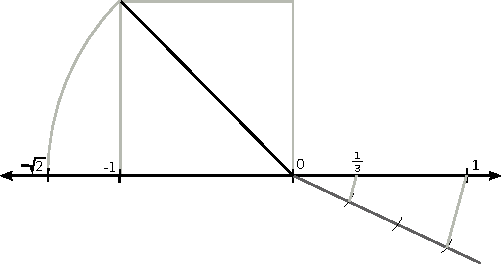
\includegraphics[width=0.8\textwidth]{slike/realrac.pdf}
  \end{center}
  \caption{Konstrukcija racionalnih in realnih števil na primeru $\frac{1}{3}$ in $-\sqrt{2}$.}
  \label{fig:real:konstr}
\end{figure}

\subsection{Intervali}
\label{sec:realna:intervali}
$\left[a,b \right] = \left\{x; a \leq x \leq b; \; x \in \R \right\}$ --- zaprt interval \\
$\left(a,b \right) = \left\{x; a < x < b; \; x \in \R \right\}$ --- odprt interval \\
$\left[a,b \right) = \left\{x; a \leq x < b; \; x \in \R \right\}$ --- polodprt interval \\
$\left(a,b \right] = \left\{x; a < x \leq b; \; x \in \R \right\}$ --- polzaprt interval \\
$(-\infty,\infty) = \R$

Predstavimo jih kot daljico na številski premici, če se daljica konča s piko je interval na tisti
strani zaprt, če se konča s puščico je odprt. Intervali so množice, tako da lahko med njimi izvajamo
enake operacije kot med množicami.

\subsection{Absolutna in relativna napaka}
\label{sec:realna:nap}
Naj bo dano določeno število $s$ in njegov približek $p$.
Absolutna napaka približka je enaka 
\[ \Delta = |s-p| \]
Relativna napaka pa je enaka
\[ \delta = \frac{\Delta}{s} \]

\section{Absolutna vrednost}
\begin{equation}
  \label{eq:abs}
  \left| x \right| = 
  \begin{cases} 
    \hfill  x; & \text{če $x \geq 0$,} \\
    \hfill -x; & \text{če $x < 0$.}
  \end{cases}
\end{equation}

\textbf{Lastnosti:}
\begin{itemize*}
  \item $|x| \geq 0$
  \item $|x| = 0 \iff x = 0$
  \item \textbf{Grafično} predstavlja oddaljenost števila od izhodišča na številski premici.
  \item $|xy| = |x| \krat |y| \quad$ Absolutna vrednost produkta je enaka produktu
    absolutnih vrednosti.
  \item $|x+y| \leq |x| + |y| \quad$ Absolutna vrednost vsote je manjša ali enaka vsoti
    absolutnih vrednosti. (\textbf{trikotniška neenakost})
\end{itemize*}

\section{Izrazi}
\label{sec:izr}
\textbf{Matematični izraz} je zapis sestavljen iz števil, spremenljivk, matematičnih funkcij in
operacij ter iz oklepajev, ki določajo vrstni red računanja. Da je tak zapis res
matematični izraz, mora biti tudi \textbf{smiseln:} Če namesto spremenljivk vstavimo konkretna
števila, mora biti možno izračunati vrednost izraza (vsaj za nekatere vrednosti
spremenljivk).
Primer:
\[ \frac{x + 1}{x} \]
Vrednost tega izraza lahko izračunamo za katero koli vrednost
spremenljivke x, razen za x = 0.

Dva matematična izraza sta \textbf{enakovredna}, če imata pri istih izbirah spremenljivk vedno
enako vrednost.
Primer: Zgornji izraz je enakovreden izrazu 
\[ 1 + \frac{1}{x} \]

Izraz \textbf{poimenujemo} glede na glavno računsko operacijo, ki v njem nastopa -- to je računska
operacija, ki jo izračunamo nazadnje.
Primeri: \\
$(x + 1)(x + 2)$ imenujemo produkt izrazov $(x + 1)$ in $(x + 2)$ \\
$5a + 3b - 2c$ imenujemo vsota izrazov $5a$, $3b$ in $-2c$ \\
$(2m + 3)^2$ imenujemo kvadrat izraza $(2m + 3)$

Izraz, v katerem nastopajo samo osnovne štiri računske operacije (seštevanje, odštevanje,
množenje in deljenje), imenujemo \textbf{aritmetični} izraz. Če v izrazu poleg tega nastopajo še
algebrske funkcije kot npr. korenjenje, je to \textbf{algebrski} izraz.

Pri preoblikovanju matematičnih izrazov pogosto uporabljamo naslednja dva postopka:
\textbf{faktorizacija} (preoblikovanje v produkt faktorjev)
\textbf{razčlenjevanje} (preoblikovanje v vsoto členov).

Formule za preoblikovanje izrazov:\\
\parbox{\textwidth}{
\begin{align}
   n \in \N, \quad & a, b, c \in \R \nonumber \\
   \label{eq:izr:kvadrat:dvoclenika} (a \pm b)^2 &= a^2 \pm 2ab + b^2 \comment{kvadrat
   dvočlenika} \\
   \label{eq:izr:kub:dvoclenika} (a \pm b)^3 &= a^3 \pm 3a^2b + 3ab^2 \pm b^3 = a^3 \pm
   b^3 + 3ab(a\pm b) \quad \footnotemark \\
   \label{eq:izr:kvadrat:troclenika} (a \pm b \pm c)^2 &= a^2 + b^2 + c^2 \pm 2ab \pm 2ac
   \pm 2bc \comment{kvadrat tročl.} \\
   \label{eq:izr:razlikakvadratov} a^2 - b^2 &= (a+b)(a-b) \comment{razlika kvadratov} \\
   \label{eq:izr:vsotakubov} a^3 \pm b^3 &= (a \pm b)(a^2 \mp ab + b^2) \comment{razlika ali
   vsota kubov} \\
   \label{eq:izr:vietovo} (x\pm a)(x\pm b) &= x^2 + (a\pm b)x \pm ab \comment{Vi\`{e}tovo
   pravilo} \\
   \label{eq:izr:ananminusbnan} a^n - b^n &= (a - b)(a^{n-1} + a^{n-2}b + \cdots
   + ab^{n-2} + b^{n-1}) \\ 
   a^n - b^n &= (a - b)\sum_{i=1}^{n} a^{n-i}b^{i-1} \nonumber \\
   \label{eq:izr:ananplubnan}  a^n + b^n &=  (a + b)(a^{n-1} - a^{n-2}b + \cdots
   - ab^{n-2} + b^{n-1}) \\
   a^n +b^n &= (a+b)\sum_{i=1}^{n} (-1)^{i+1}a^{n-i}b^{i-1} \comment{za lihe $n$} \nonumber
\end{align}
}
\footnotetext{Kub dvočlenika.}

\section{Potence}
\label{sec:pot}
\subsection{Potence z naravnim eksponentom}
\label{sec:pot:nar}
So krajši zapis za množenje več enakih faktorjev.
\begin{equation}
    a^n = \underbrace{a \krat a \krat a \krat a \krat \cdots \krat a}_n
    \label{eq:pot:defn}
\end{equation}

\subsubsection{Pravila za računanje}
\label{sec:pot:nar:prav}
Vsa pravila se dokaže tako, da se potenco zamenja po definiciji \eqref{eq:pot:defn} in
pogleda število faktorjev.
\begin{align}
  a^m \krat a^n &= a^{m+n} \label{eq:pot:anankratanam} \\
  (a^m)^n &= a^{m\krat n} \label{eq:pot:anannam} \\
  (a\krat b)^n &= a^n \krat b^n \label{eq:pot:akratbnan}
\end{align}

\subsection{Potence s celim eksponentom}
\label{sec:pot:cela}
\begin{equation}
  \label{eq:pot:defz}
  a^k =
  \begin{cases}
    \hfill a^k; & \text{če $k > 0$ (po definiciji \eqref{eq:pot:defn})} \\
    \hfill 1;   & \text{če $k = 0$} \\
    \hfill \frac{1}{a^{-k}}; & \text{če $k < 0$}
  \end{cases}
  \qquad k \in \Z
\end{equation}


\subsubsection{Pravila za računanje}
\label{sec:pot:cela:prav}
Veljajo vsa pravila kot za naravna števila (razdelek \ref{sec:pot:nar:prav}). Poleg teh veljajo še
naslednja pravila, ki se dokažejo podobno kot pri naravnih eksponentih:
\begin{align}
  \frac{a^n}{a^m} &= a^{n-m} \label{eq:pot:anandelanam} \\
  \frac{a^n}{b^n} &= \left( \frac{a}{b} \right)^n
\end{align}

\subsection{Potence z racionalnim eksponentom}
\label{sec:pot:rac}
V tem razdelku se uporabljajo koreni in pravila za računanje z njimi. Koreni so opisani
kasneje v razdelku \ref{sec:kor}, pravila pa v razdelku \ref{sec:kor:prav}.
\begin{equation}
  \label{eq:pot:defrac}
  a^{\frac{m}{n}} = \sqrt[n]{a^m}; \quad a \in \R^+ \cup \left\{ 0 \right\}; \; m \in \Z;
  \; n \in \Z - \left\{ 0 \right\}
\end{equation}

\subsubsection{Pravila za računanje}
\label{sec:pot:rac:prav}
\begin{align}
  a^{\frac{m}{n}} \krat a^{\frac{q}{p}} &= a^{\frac{mp+qn}{np}} \label{eq:pot:rac:prav:prodpot} \\
  \frac{a^{\frac{m}{n}}}{a^{\frac{q}{p}}} &= a^{\frac{mp-qn}{np}} \label{eq:pot:rac:prav:kvocpot} \\
  \left( a^{\frac{m}{n}} \right)^{\frac{q}{p}} &= a^{\frac{mq}{np}} \label{eq:pot:rac:prav:potpot} \\
  \left( a \krat b \right)^{\frac{m}{n}} &= a^{\frac{m}{n}} \krat b^{\frac{m}{n}}
  \label{eq:pot:rac:prav:potprod} \\
  \left( \frac{a}{b} \right)^{\frac{m}{n}} &= \frac{a^{\frac{m}{n}}}{b^{\frac{m}{n}}}
  \label{eq:pot:rac:prav:potkvoc} \\
\end{align}

Dokaz pravila \ref{eq:pot:rac:prav:prodpot}:
\[ a^{\frac{m}{n}} \krat a^{\frac{q}{p}} = \sqrt[n]{a^m} \krat \sqrt[p]{a^q} =
\sqrt[np]{a^{mp+qn}} = a^{\frac{mp+qn}{np}} \comment{pravilo za računanje s
koreni \eqref{eq:kor:prav:prodkor}} \]

Dokaz pravila \ref{eq:pot:rac:prav:kvocpot}:
\[ \frac{a^{\frac{m}{n}}}{a^{\frac{q}{p}}} = \frac{\sqrt[n]{a^m}}{\sqrt[p]{a^q}} =
\sqrt[np]{a^{mp-qn}} = a^{\frac{mp-qn}{np}} \comment{pravilo za računaje s koreni
\eqref{eq:kor:prav:kvockor}} \]

Dokaz pravila \ref{eq:pot:rac:prav:potpot}:
\[ \left( a^{\frac{m}{n}} \right)^{\frac{q}{p}} = \sqrt[p]{\left(\sqrt[n]{a^m} \right)^q}
= \sqrt[np]{a^{mq}} = a^{\frac{mq}{np}} \comment{pravilo za računanje s koreni
\eqref{eq:kor:prav:korkoranannaq}}\]

Dokaz pravila \ref{eq:pot:rac:prav:potprod}:
\[ \left( a \krat b \right)^{\frac{m}{n}} = \sqrt[n]{\left( a \krat b\right)^m} =
\sqrt[n]{a^m \krat b^m} = \sqrt[n]{a^m} \krat \sqrt[n]{b^m} = a^{\frac{m}{n}} \krat
b^{\frac{m}{n}} \comment{up. pravilo \eqref{eq:kor:prav:prodenakkor}} \]

Dokaz pravila \ref{eq:pot:rac:prav:potkvoc}:
\[ \left( \frac{a}{b} \right)^{\frac{m}{n}} = \sqrt[n]{\left( \frac{a}{b} \right)^m} =
\sqrt[n]{\frac{a^m}{b^m}} = \frac{\sqrt[n]{a^m}}{\sqrt[n]{b^m}} =
\frac{a^{\frac{m}{n}}}{b^{\frac{m}{n}}} \comment{uporabljeno pravilo \eqref{eq:kor:prav:ulenakkor}}
\]
\section{Koreni}
\label{sec:kor}
\begin{equation}
  \label{eq:kor:def}
  \sqrt[n]{a} = b \iff b^n = a; \quad a, b \in \R^+ \cup \{0\}, \; n \in \Z - \{0\}
\end{equation}
Če $a \in \R^-$: \\
če $n$ lih: $\sqrt[n]{a} = -\sqrt[n]{|a|}$ \\
če $n$ sod: ne obstaja v realnem.\\

Dogovor:
\begin{align*}
  \sqrt[2]{a} &= \sqrt{a}
\end{align*}

Osnovne izpeljave:
\begin{align}
  \sqrt[1]{a} &= a \nonumber \\
  \sqrt[n]{a^n} &= a \label{eq:kor:dog:nkorn} \\
  \left(\sqrt[n]{a}\right)^n &= a \label{eq:kor:dog:nkornzakn}
\end{align}

\subsection{Pravila za računanje}
\label{sec:kor:prav}
\begin{align}
  \sqrt[n]{a^m} &= \sqrt[p]{a^q} \iff mp = qn \label{eq:kor:prav:mpjeqn} \\
  \sqrt[n]{a^m} &= \sqrt[nx]{a^{mx}} \label{eq:kor:prav:razsirjanje} \\ 
  \sqrt[n]{a} \krat \sqrt[n]{b} &= \sqrt[n]{a \krat b} \label{eq:kor:prav:prodenakkor} \\
  \frac{\sqrt[n]{a}}{\sqrt[n]{b}} &= \sqrt[n]{\frac{a}{b}} \label{eq:kor:prav:ulenakkor} \\
  \sqrt[n]{a^m} \krat \sqrt[p]{a^q} &= \sqrt[np]{a^{mp+qn}} \label{eq:kor:prav:prodkor} \\
  \frac{\sqrt[n]{a^m}}{\sqrt[p]{a^q}} &= \sqrt[np]{a^{mp-qn}} \label{eq:kor:prav:kvockor} \\
  \sqrt[p]{\sqrt[n]{a}} &= \sqrt[np]{a} \label{eq:kor:prav:korkor} \\
  \left( \sqrt[n]{a^m} \right)^q &= \sqrt[n]{a^{mq}}  \label{eq:kor:prav:koranannaq} \\
  \sqrt[p]{\left( \sqrt[n]{a^m} \right)^q} &= \sqrt[np]{a^{mq}} \label{eq:kor:prav:korkoranannaq}
\end{align}

Pri dokazih se uporabljajo pravila za računanje s potencami s celim eksponentom (razdelek
\ref{sec:pot:cela:prav}).\\[5pt]
Dokaz pravila \ref{eq:kor:prav:mpjeqn}:
\begin{align*}
  \sqrt[n]{a^m} &= \sqrt[p]{a^q} \comment{$^{np}$} \\
  \left(\sqrt[n]{a^m}\right)^{np} &= \left(\sqrt[p]{a^q} \right)^{np} \comment{upoštevamo
  osnovno izpeljavo \eqref{eq:kor:dog:nkornzakn}} \\
  \left( a^m \right)^p &= \left( a^q \right)^n \\
  a^{mp} &= a^{qm} \\
  mp &= qn
\end{align*}

Dokaz pravila \ref{eq:kor:prav:razsirjanje}:
\begin{align*}
  \sqrt[n]{a^m} &= \sqrt[nx]{a^{mx}} \\
  mnx &= nmx \comment{glej pravilo \eqref{eq:kor:prav:mpjeqn}}
\end{align*}

Dokaz pravila \ref{eq:kor:prav:prodenakkor}:
\begin{align*}
  \sqrt[n]{a} \krat \sqrt[n]{b} &= x \\
  \left( \sqrt[n]{a} \krat \sqrt[n]{b} \right)^n &= x^n \\
  \left(\sqrt[n]{a}\right)^n \krat \left(\sqrt[n]{b} \right)^n &= x^n \\
  a \krat b &= x^n \\
  x &= \sqrt[n]{a\krat b} \comment{upoštevamo definicijo korena \eqref{eq:kor:def}}
\end{align*}

Dokaz pravila \ref{eq:kor:prav:ulenakkor}:
\begin{align*}
  \frac{\sqrt[n]{a}}{\sqrt[n]{b}} &= x \\
  \left( \frac{\sqrt[n]{a}}{\sqrt[n]{b}} \right)^n &= x^n \\
  \frac{\left( \sqrt[n]{a} \right)^n}{\left( \sqrt[n]{b} \right)^n} &= x^n \\
  \frac{a}{b} &= x^n \\
  x &= \sqrt[n]{\frac{a}{b}} \comment{upoštevamo definicijo korena \eqref{eq:kor:def}}
\end{align*}

Dokaz pravila \ref{eq:kor:prav:prodkor}:
\begin{align*}
  \sqrt[n]{a^m} \krat \sqrt[p]{a^q} &= x \comment{$^{np}$} \\
  \left( a^m \right)^p \krat \left( a^q \right)^n &= x^{np} \\
  a^{mp} \krat a^{qn} &= x^{np} \\
  a^{mp + qn} &= x^{np} \\
  x &= \sqrt[np]{a^{mp+qn}} \comment{upoštevamo definicijo korena \eqref{eq:kor:def}}
\end{align*}

Dokaz pravila \ref{eq:kor:prav:kvockor}:
\begin{align*}
  \frac{\sqrt[n]{a^m}}{\sqrt[p]{a^q}} &= x \; ^{np} \\
  \frac{a^{mp}}{a^{qn}} &= x^{np} \\
  a^{mp-qn} &= x^{np} \\
  x &= \sqrt[np]{a^{mp-qn}} \comment{upoštevamo definicijo korena \eqref{eq:kor:def}}
\end{align*}

Dokaz pravila \ref{eq:kor:prav:korkor}:
\begin{align*}
   \sqrt[p]{\sqrt[n]{a}} &= x \\
   \sqrt[n]{a} &= x^p \\
   a &= \left( x^p \right)^n \\
   a &= x^{np} \\
   x &= \sqrt[np]{a} \comment{upoštevamo definicijo korena \eqref{eq:kor:def}}
\end{align*}

Dokaz pravila \ref{eq:kor:prav:koranannaq}:
\begin{align*}
  \left( \sqrt[n]{a^m} \right)^q &= x \\
  \left( \sqrt[n]{a^m} \right)^{qn} &= x^n \comment{upoštevamo osnovno izpeljavo \eqref{eq:kor:dog:nkornzakn}} \\
  \left( a^m \right)^q &= x^n \\
  a^{mq} &= x^n \\
  x &= \sqrt[n]{a^{mq}}
\end{align*}

Dokaz pravila \ref{eq:kor:prav:korkoranannaq}:
\[  \sqrt[p]{\left( \sqrt[n]{a^m} \right)^q} = \sqrt[p]{\sqrt[n]{a^{mq}}} =
\sqrt[np]{a^{mq}} \comment{upoštevamo pravili \eqref{eq:kor:prav:korkor} in
\eqref{eq:kor:prav:koranannaq}.} \]

\section{Logaritmi}
\label{sec:log}
\begin{equation}
  \label{eq:log:def}
  \log_a\! x = y \iff a^y = x 
\end{equation}

Osnovne izpeljave iz definicije:
\begin{align}
  \log_a\! a &= 1 \label{eq:log:logaaje1} \\
  \log_a\! 1 &= 0 \label{eq:log:log1je0} \\
  a^{\log_a\! x} &= x \label{eq:log:analogax} \\
  \log_a\! a^y &= y \label{eq:log:logaanay}
\end{align}

Dogovora:
\begin{align*}
  \log_{10}\!x &= \log x \\
  \log_{e}\!x &= \ln x
\end{align*}

\vspace{-24pt}
\hspace{100pt}
\footnote{Matematiki za logaritem z osnovo $e$ pogosto uporabljajo
kar zapis $\log x$.}

\subsection{Pravila za računanje}
\label{sec:eq:log:prav}
Logaritem \textbf{potence} je enak produktu med eksponentom in logaritmom osnove:
\begin{equation}
  \log_a\! x^n = n\log_a\! x \label{eq:log:prav:loganan}
\end{equation}
Logaritem \textbf{produkta} je enak vsoti logaritmov posameznih faktorjev:
\begin{equation}
  \log_a\! xy = \log_a\!x+ \log_a\!y \label{eq:log:prav:logprod}
\end{equation}
Logaritem \textbf{kvocienta} je enak razliki med logaritmom števca in imenovalca:
\begin{equation}
  \log_a\!\frac{x}{y} = \log_a\!x-\log_a\!y \label{eq:log:prav:logkvoc}
\end{equation}

Dokaz pravila \ref{eq:log:prav:loganan} (upoštevamo osnovni izpeljavi \eqref{eq:log:analogax} in
\eqref{eq:log:logaanay}):
\[ \log_a\!x^n = \log_a\!\left( a^{\log_a\!x} \right)^n = \log_a\!\left( a^{n\log_a\!x}
\right) = n \krat \log_a\!x  \]

Dokaz pravila \ref{eq:log:prav:logprod} (upoštevamo osnovni izpeljavi \eqref{eq:log:analogax} in
\eqref{eq:log:logaanay}):
\[ \log_a\!xy = \log_a\!\left( a^{\log_a\!x} \krat a^{\log_a\!y} \right) = \log_a\!\left(
a^{\log_a\!x+\log_a\!y} \right) = \log_a\!x + \log_a\!y \]

Dokaz pravila \ref{eq:log:prav:logkvoc} (upoštevamo pravili \eqref{eq:log:prav:logprod}  in
\eqref{eq:log:prav:loganan}):
\[ \log_a\!\frac{x}{y} = \log_a\!xy^{-1} = \log_a\!x + \log_a\!y^{-1} = \log_a\!x -
\log_a\!y \]

Prehod na novo osnovo:
\begin{align*}
  \log_b\!a^y &= \log_b\!x \comment{po definiciji \eqref{eq:log:def} je $a^y$ enak $x$} \\
  y \krat \log_b\!a &= \log_b\!x \comment{uporabimo pravilo \eqref{eq:log:prav:loganan}} \\
  y &= \frac{\log_b\!x}{\log_b\!a} \\
  \log_a\!x &= \frac{\log_b\!x}{\log_b\!a} \comment{po definiciji je $y$ enak $\log_a\!x$}
\end{align*}
Iz tega izpeljemo zvezo:
\[ \log_a\!x = \frac{1}{\log_x\!a} \]

\section{Koordinatni sistem}
\label{sec:koor}
\subsection{Pravokotni, v ravnini}
\label{sec:koor:pravrav}
Dve pravokotni osi. \\
$x$ --- abscisna os \\
$y$ --- ordinatna os
\[ \mathcal{M} = \left\{ (x,y); \; x, y \in \R \right\} = \R \times \R = \R^2 \]

Glej tudi sliko~\ref{fig:koor:prav}.

\begin{figure}[ht]
  \begin{center}
      \begin{pspicture*}(-3.5,-3.5)(3.5,3.5)
        \psaxes[]{->}(0,0)(-3.5,-3.5)(3.5,3.5)
        \psdots(2,1)
        \uput[ur](2,1){$T(x,y)$}
        \uput[dl](0,0){$0$}
        \uput[r](0,3){$y$}
        \uput[u](3,0){$x$}
        \uput[ur](2,2){\Rom{1}.}
        \uput[ul](-2,2){\Rom{2}.}
        \uput[dl](-2,-2){\Rom{3}.}
        \uput[dr](2,-2){\Rom{4}.}
      \end{pspicture*}
  \end{center}
  \beforecaptionskip
  \caption{Pravokotni koordinatni sistem.}
  \label{fig:koor:prav}
\end{figure}

Osi razdelita ravnino na štiri \textbf{kvadrante}: \\[3pt]
\begin{tabular}{ll}
  \Rom{1}. kvadrant: & $x > 0 \land y > 0$ \\
  \Rom{2}. kvadrant: & $x < 0 \land y > 0$ \\
  \Rom{3}. kvadrant: & $x < 0 \land y < 0$ \\
  \Rom{4}. kvadrant: & $x > 0 \land y < 0$ \\
\end{tabular}
\\
Pomembni \textbf{premici}:
\begin{align*}
  y &= x  \comment{simetrala lihih kvadrantov} \\
  y &= -x \comment{simetrala sodih kvadrantov}
\end{align*}

\textbf{Pas:} $a < x < b$ 

\textbf{Razdalja} med dvema točkama (dokaz: Pitagorov izrek):
\begin{align*}
  A(x_1, y_1) \\
  B(x_2, y_2) \\
  d(A,B) &= \sqrt{\left( x_2 - x_1 \right)^2 + \left( y_2 - y_1 \right)^2}
\end{align*}

\textbf{Središče} daljice:
\[ S_{AB} = \left( \frac{x_a+x_b}{2}, \frac{y_a+y_b}{2} \right) \]

\textbf{Težišče} in \textbf{ploščina} trikotnika\footnote{Za razrešitev
determinante matrike glej enačbo \eqref{eq:koor:determinanta}. In ja, |\ \ | ne pomeni absolutne
vrednosti.}:
\[ T_{ABC} = \left( \frac{x_a+x_b+x_c}{3},\frac{y_a+y_b+y_c}{3} \right) \]
\[ p\sigma = \frac{1}{2} \begin{vmatrix}
    x_2 - x_1 & y_2 - y_1 \\
    x_3 - x_1 & y_3 - y_1 
\end{vmatrix} \comment{$\sigma$ je orientacija trikotnika.} \]
\[ p\sigma = \frac{1}{2} \left[ (x_2-x_1)(y_3-y_1) + (y_2-y_1)(x_3-x_1) \right] \]
\[ p\sigma = \frac{1}{2} \left[ x_1(y_2-y_3 + x_2(y_3-y_1) + x_3(y_1-y_2) \right] \]

Determinanta:
\begin{equation}
  \begin{vmatrix}
    a & b \\
    c & d
  \end{vmatrix} = a \krat d - b \krat c
  \label{eq:koor:determinanta}
\end{equation}

\subsection{Pravokotni, v prostoru}
\label{sec:koor:pravpro}
Dve pravokotni osi. \\
$x$ --- abscisna os \\
$y$ --- ordinatna os \\
$z$ --- aplikatna os
\[ \mathcal{M} = \left\{ (x,y,z); \; x, y, z \in \R \right\} = \R \times \R \times \R = \R^3 \]

Formule so enake kot v ravnini (razdelek \ref{sec:koor:pravrav}), le da vsebujejo še
tretjo koordinato.

\subsection{Polarni, v ravnini}
\label{sec:koor:pol}
Za polarni koordinatni sistem potrebujemo izhodišče, poltrak in enoto. Točka je enolično
določena z oddaljenostjo od izhodišča in pozitivnim kotom od poltraka. Polarni koordinatni
sistem je prikazan pa sliki~\ref{fig:koor:pol}.
\[ T(r,\varphi); \; r \ge 0; \; 0 \le \varphi \le 2\pi \]

\begin{figure}[ht]
  \begin{center}
      \begin{pspicture*}(-3.5,-3.5)(3.5,3.5)
        \psdots(0,0)(2,1)(1,0)
        \psline(0,0)(3.5,0)
        \psline(0,0)(2,1)
        \pscurve{->}(1.5,0)(1.46,.3)(1.3,.65)
        \uput[dl](0,0){$0$}
        \uput[d](1,0){$1$}
        \uput[d](3.2,0){$p$}
        \uput[ur](2,1){$T(r,\varphi)$}
        \uput[u](1,0.5){$r$}
        \uput[r](0.75, 0.25){$\varphi$}
      \end{pspicture*}
  \end{center}
  \beforecaptionskip
  \caption{Polarni koordinatni sistem.}
  \label{fig:koor:pol}
\end{figure}

Pretvarjanje med kartezičnim in polarnih sistemom je možno. Držijo naslednje enakosti
(za razlago glej sliko~\ref{fig:koor:pretv}):
\begin{align*}
  & r^2 = x^2 + y^2 \\
  & \tan\varphi = \frac{y}{x} \\
  & x = r\krat\kos\varphi \\
  & y = r\krat\sin\varphi \\
\end{align*}

\begin{figure}[ht]
  \begin{center}
      \begin{pspicture*}(-3.5,-3.5)(3.5,3.5)
        \psaxes[labels=none]{->}(0,0)(-1.5,-1.5)(3.5,3.5)
        \uput[dl](0,0){$0$}
        \psdots(2,1.5)(0,0)
        \uput[ur](2,1.5){$T(x,y)$}
        \uput[-25](2,1.5){$T(r,\varphi)$}
        \uput[ul](2,1.5){$z$}
        \uput[u](2.85,0){$x$}
        \uput[u](3.15,-.08){$p$}
        \uput[r](0,3){$y$}
        \uput[d](3,0){$\Re$}
        \uput[l](0,3){$\Im$}
        \psline(0,0)(2,1.5)
        \rput*[b]{36.87}(1,.9){$r = |z|$}
        \oznaka(2,0)(2,1.5)
        \uput[r](0.75, 0.3){$\varphi$}
        \pscurve{->}(1.5,0)(1.40,.5)(1.2,.9)
        \uput[d](1.5,0){$x$}
        \uput[r](2,.75){$y$}
        \psline[linewidth=.5pt](1.8,0)(1.8,.2)(2,.2) % pravi kot
      \end{pspicture*}
  \end{center}
  \beforecaptionskip
  \caption{Pretvarjanje med koordinatnima sistemoma in kompleksno ravnino.}
  \label{fig:koor:pretv}
\end{figure}

\subsubsection{Polarni zapis kompleksnega števila}
Kompleksno število predstavimo kot točko v koordinatnem sistemu. Po formulah za
pretvarjanje med sistemoma ugotovimo (glej sliko~\ref{fig:koor:pretv}):
\begin{align*}
  z &= x + y\ii \\
  z &= r\kos\varphi + r\sin\varphi \krat \ii \\
  z &= \left|z\right|\left( \kos\varphi+\ii\sin\varphi \right) \\
\end{align*}

Formula za potenciranje kompleksnega števila z naravnim številom (dokažemo s popolno
indukcijo):
\[ z^n = |z|^n(\kos n\varphi + \ii\sin n\varphi) \]

\section{Funkcije}
\label{sec:fun}
\[ f(x)\!: A \rightarrow B \]
\textbf{Funkcija}, ki množico $A$ preslika v množico $B$ je predpis, ki vsakemu elementu iz množice
$A$ priredi natanko določen element iz množice $B$.
\[ f(x)\!: A \rightarrow B; \; A, B \subseteq \R \]
Funkcija je \textbf{realna}, če podmnožico realnih števil preslika v podmnožico realnih števil.

\textbf{Definicijsko območje} ($D_f$) funkcije $f$ je množica realnih števil, za katera lahko
predpis izračunamo.

\textbf{Zaloga vrednosti} ($Z_f$) funkcije $f$ je množica realnih števil, ki jih funkcija lahko
zavzame.

\textbf{Graf} ($G_f$) funkcije $f$ je množica urejenih parov $(x, y)$, pri katerih je $x$ element
definicijskega območja, $y$ pa vrednost funkcije pri $x$.
\[ G_f = \left\{ (x,y); \; x \in D_f, \; y = f(x) \right\} \]

$a$ je \textbf{ničla} funkcije, če je vrednost funkcije pri $a$ enaka 0.
\[ a \textnormal{ ničla } \iff f(a) = 0 \]

\textbf{Začetna vrednost} funkcije je vrednost funkcije pri 0.
\[ \textnormal{začetna vrednost} = f(0) \]

Funkcija je \textbf{padajoča}, če pri vsakem večjem $x$ zavzame manjšo vrednost.
\[ f(x) \textnormal{ padajoča } \iff \forall x_1, x_2 \in D_f: x_1 < x_2 \implies f(x_1) >
f(x_2) \]

Funkcija je \textbf{naraščajoča}, če pri vsakem večjem $x$ zavzame večjo vrednost.
\[ f(x) \textnormal{ naraščajoča } \iff \forall x_1, x_2 \in D_f: x_1 < x_2 \implies f(x_1) <
f(x_2) \]

Funkcija je \textbf{navzgor omejena}, če so vse funkcijske vrednosti manjše ali enake od nekega
realnega števila $M$ (zgornja meja).
\[ f(x) \textnormal{ navzgor omejena } \iff \exists M \in \R: f(x) \leq M; \forall x \in D_f \]


Funkcija je \textbf{navzdol omejena}, če so vse funkcijske vrednosti večje ali enake od nekega
realnega števila $m$ (spodnja meja).
\[ f(x) \textnormal{ navzdol omejena } \iff \exists m \in \R: f(x) \geq m; \forall x \in D_f \]

Funkcija je \textbf{omejena}, če je omejena navzgor in navzdol.

\textbf{Pol} je realno število, za katerega funkcija ni definirana, v njegovi bližini pa funkcija
narašča ali pada čez vse meje (proti $\infty$ ali $-\infty$). 

\textbf{Asimptota} je krivulja, ki se ji graf približuje pri po absolutni vrednosti velikih
vrednostih neodvisne spremenljivke.

Funkcija je na nekem območju \textbf{konveksna}, če za vsaki dve točki na grafu funkcije
velja, da leži graf pod daljico, ki jo določata ti dve točki.

Funkcija je na nekem območju \textbf{konkavna}, če za vsaki dve točki na grafu funkcije velja, da
leži graf nad daljico, ki jo določata ti dve točki.

Funkcija je \textbf{soda}, če za vsak $x$ iz definicijskega območja velja: $f(-x) = f(x)$.
Graf sode funkcije je simetričen glede na $y$ os.
\[ f(x) \textnormal{ soda } \iff f(-x) = f(x); \; \forall x \in D_f \]

Funkcija je \textbf{liha}, če za vsak $x$ iz definicijskega območja velja: $f(-x) = -f(x)$.
Graf lihe funkcije je središčno simetričen glede na koordinatno izhodišče.
\[ f(x) \textnormal{ liha } \iff f(-x) = -f(x); \; \forall x \in D_f \]

Funkcija je na nekem območju \textbf{pozitivna}, če so vse funkcijske vrednosti na tem območju
večje od 0.

Funkcija je na nekem območju \textbf{negativna}, če so vse funkcijske vrednosti na tem območju
manjše od 0.

Funkcija je \textbf{periodična} natanko takrat, ko obstaja tak $\omega \in \R^+$, da za vsak $x$ iz
definicijskega območja velja $f(x) = f(x+\omega)$.
\[ f(x) \textnormal{ periodična } \iff \exists \omega \in \R^+: f(x) = f(x+\omega), \; \forall x \in
D_f \comment{$\omega$ --- perioda} \]

\textbf{Val} periodične funkcije je del funkcije na intervalu $[x, x+\omega), x \in D_f$.

\subsection{Premik funkcije}
\label{sec:fun:prem}
Funkcijo $y = f(x)$ premaknemo za vektor $\vec{v} = (p,q)$ (glej sliko~\ref{fig:fun:prem}).
\begin{align*}
  x &= x'-p \\
  y &= y'-q \\
  y &= f(x) \\
  y' - q &= f(x'-p) \\
  y' &= f(x'-p) + q
\end{align*}
Parameter $p$ vpliva na \textbf{premik}
po $x$ osi (levo -- desno), parameter $q$ pa na premik po $y$ osi (gor -- dol).

\begin{figure}[ht]
  \begin{center}
      \begin{pspicture*}(-3.5,-3.5)(3.5,3.5)
        \psaxes[labels=none]{->}(0,0)(-3.5,-3.5)(3.5,3.5)
        \psplot[plotstyle=curve,linecolor=black, linewidth=.5pt]{-3.5}{3.5}{x -1 mul 3 exp}
        \psplot[plotstyle=curve,linecolor=black, linewidth=.5pt]{-3.5}{3.5}{x 2 sub -1 mul 3 exp 1 add}
        \psline[linecolor=black, linewidth=1pt]{->}(-1,1)(1,2)
        \oznaka(-1,1)(0,1)
        \oznaka(-1,1)(-1,0)
        \oznaka(1,2)(0,2)
        \oznaka(1,2)(1,0)
        \uput[r](0,1){$y$}
        \uput[l](0,2){$y'$}
        \uput[d](-1,0){$x$}
        \uput[d](1,0){$x'$}
        \uput[l](-1,1){$T(x,y)$}
        \uput[60](-1,1){$\vec{v}$}
        \uput[45](1,2){$T'(x',y')$}
      \end{pspicture*}
  \end{center}
  \beforecaptionskip
  \caption{Premik funkcije.}
  \label{fig:fun:prem}
\end{figure}

\subsection{Razteg funkcije}
\label{sec:fun:razt}
Funkcijo $y = f(x)$ raztegnemo s parametroma $a$ in $b$.
\[ y = a \krat f\left( \frac{x}{b} \right) \]
Parameter $a$ predstavlja razteg v smeri $y$ osi, če je negativen, se graf preslika čez
$x$ os. Odvisnost funkcije od parametra $a$ je prikazana na sliki~\ref{fig:fun:a}. 

Parameter $b$ predstavlja razteg v smeri $x$ osi, če je negativen, se graf
preslika čez $y$ os. Odvisnost funkcije od parametra $b$ je prikazana na sliki~\ref{fig:fun:b}. 

\begin{figure}[ht]
  \begin{center}
    \subfigure[Parameter $a$.]{
      \label{fig:fun:a}
      \begin{pspicture*}(-3.5,-3.5)(3.5,3.5)
        \psaxes[labels=none]{->}(0,0)(-3.5,-3.5)(3.5,3.5)
        \psplot[plotstyle=curve,linecolor=black, linewidth=1pt]{-3.5}{3.5}{x 2 exp}
        \psplot[plotstyle=curve,linecolor=blue, linewidth=1pt]{-3.5}{3.5}{x 2 exp 4 mul}
        \psplot[plotstyle=curve,linecolor=red, linewidth=1pt]{-3.5}{3.5}{x 2 exp 0.3 mul}
        \psplot[plotstyle=curve,linecolor=green, linewidth=1pt]{-3.5}{3.5}{x 2 exp -1 mul}
        \uput[r](1.8,3){$1$}
        \uput[r](0.8,3){$4$}
        \uput[r](2,1){$0,3$}
        \uput[r](1.8,-3){$-1$}
      \end{pspicture*}
    }
    \subfigure[Parameter $b$.]{
      \label{fig:fun:b}
      \begin{pspicture*}(-3.5,-3.5)(3.5,3.5)
        \psaxes[labels=none]{->}(0,0)(-3.5,-3.5)(3.5,3.5)
        \psplot[plotstyle=curve,linecolor=black, linewidth=1pt]{-3.5}{3.5}{x 3 exp}
        \psplot[plotstyle=curve,linecolor=blue, linewidth=1pt]{-3.5}{3.5}{x 2.5 div 3 exp}
        \psplot[plotstyle=curve,linecolor=red, linewidth=1pt]{-3.5}{3.5}{x 0.3 div 3 exp}
        \psplot[plotstyle=curve,linecolor=green, linewidth=1pt]{-3.5}{3.5}{x -1 div 3 exp}
        \uput[r](1.5,3){$1$}
        \uput[r](0.4,3){$0,3$}
        \uput[r](2.5,1){$2,5$}
        \uput[r](-1.5,3){$-1$}
      \end{pspicture*}
    }
  \end{center}
  \beforecaptionskip
  \caption{Odvisnost funkcije od parametrov $a$ in $b$.}
  \label{fig:fun:ab}
\end{figure}

\subsection{Inverzna funkcija}
\label{sec:fun:inv}
\textbf{Inverzna funkcija} funkcije $f(x)$ je funkcija $f^{-1}(x)$, ki jo dobimo tako, da v prvotni
funkciji zamenjamo vlogo odvisne in neodvisne spremenljivke, ter izrazimo novo neodvisno
spremenljivko. \textbf{Grafično} dobimo graf $f^{-1}(x)$ tako, da graf prvotne funkcije preslikamo
čez simetralo lihih kvadrantov. Inverzno funkcijo lahko dobimo samo na območjih, ko je
prvotna funkcija \textbf{injektivna}.\footnote{Za definicijo injektivnosti glej razdelek
\ref{sec:preslikave}.}

\subsection{Linearna funkcija}
\textbf{Linearna funkcija} je vsaka funkcija oblike $y = kx + n; \; k, n \in \R$.
Graf linearne funkcije je premica. Funkcijski predpis lahko zapišemo v treh oblikah:
\label{sec:fun:lin}
\begin{align*}
  y = kx + n \comment{eksplicitna,} \\
  ax + by + c = 0 \comment{implicitna,} \\
  \frac{x}{m} + \frac{y}{n} = 1 \comment{odsekovna enačba premice}
\end{align*}
V eksplicitni obliki ne moremo napisati premic vzporednih z ordinatno osjo, v odsekovni
obliki pa ne moremo napisati premic, ki so vzporedne katerikoli izmed osi ali gredo skozi
izhodišče koordinatnega sistema.

$k$ --- smerni koeficient \\
$n$ --- začetna vrednost, odsek na ordinatni osi \\
$m$ --- odsek na abscisni osi

Osnovni Evklidov aksiom: Skozi dve točki lahko potegnemo natanko eno premico.
\textbf{Smerni koeficient} premice skozi dve točki se izračuna kot razmerje med razliko v smeri $y$
in razliko v smeri $x$ osi.
\[ k = \frac{y_2 - y_1}{x_2 - x_1} \]
Če je smerni koeficient večji od 0 je premica naraščajoča, če je manjši od 0, je premica
padajoča.

Družina premic ki so \textbf{vzporedne} premici $y = k_1x+n_1$: $y=k_1x+n_2$ \\
Družina premic, ki gredo skozi \textbf{točko} $T_0(x_0,y_0)$: $y - y_0 = k(x-x_0)$ 

\textbf{Vzporedna} premica dani premici ima enak $k$ kot podana, $k$ premice, ki je na dano premico
\textbf{pravokotna}, pa je nasprotno in obratno število smernemu koeficientu dane premice.
\[ k_2 = -\frac{1}{k_1} \]

\textbf{Razdalja točke} $T(x_0, y_0)$ od \textbf{premice} $p\;(ax+by-c=0)$:
\[ d(p, T) = \left|\frac{ax_0+by_0-c}{\sqrt{a^2+b^2}}\right|  \]

\textbf{Snop} premic je prikazan na sliki~\ref{fig:fun:lin:snop}, \textbf{šop} premic na sliki~\ref{fig:fun:lin:sop}.

\begin{figure}[ht]
  \begin{center}
    \subfigure[Snop premic.]{
      \label{fig:fun:lin:snop}
      \begin{pspicture*}(-2.0,-2.0)(2.0,2.0)
        \psaxes[labels=none]{->}(0,0)(-2.0,-1.99)(2.0,2.0)
        \psplot[plotstyle=curve,linecolor=black, linewidth=1pt]{-2.0}{2.0}{x}
        \psplot[plotstyle=curve,linecolor=black, linewidth=1pt]{-2.0}{2.0}{x 1.5 sub}
        \psplot[plotstyle=curve,linecolor=black, linewidth=1pt]{-2.0}{2.0}{x 0.5 add}
        \psplot[plotstyle=curve,linecolor=black, linewidth=1pt]{-2.0}{2.0}{x 1.5 add}
      \end{pspicture*}
    }
    \subfigure[Šop premic.]{
      \label{fig:fun:lin:sop}
      \begin{pspicture*}(-2.0,-2.0)(2.0,2.0)
        \psaxes[labels=none]{->}(0,0)(-2.0,-1.99)(2.0,2.0)
        \psplot[plotstyle=curve,linecolor=black, linewidth=1pt]{-2.0}{2.0}{x 0.5 add}
        \psplot[plotstyle=curve,linecolor=black, linewidth=1pt]{-2.5}{2.5}{x 0.5 add 0.5 mul}
        \psplot[plotstyle=curve,linecolor=black, linewidth=1pt]{-2.5}{2.5}{x 0.5 add -2 mul}
        \psplot[plotstyle=curve,linecolor=black, linewidth=1pt]{-2.5}{2.5}{x 0.5 add -0.5 mul}
      \end{pspicture*}
    }
  \end{center}
  \beforecaptionskip
  \caption{Posebni medsebojni legi premic.}
  \label{fig:fun:lin:snopsop}
\end{figure}

\subsection{Potenčna funkcija}
\label{sec:fun:pot}
\textbf{Potenčna funkcija} je vsaka funkcija oblike: $f(x) = x^n; \; n \in \Z  - \left\{ 0,1 \right\}$.
Poznamo štiri glavne \textbf{grafe} potenčne funkcije, ki se delijo glede na eksponent:
\begin{itemize*}
  \item pozitiven sod eksponent (slika~\ref{fig:fun:pot:sodplus})
  \item pozitiven lih eksponent (slika~\ref{fig:fun:pot:lihplus})
  \item negativen sod eksponent (slika~\ref{fig:fun:pot:sodminus})
  \item negativen lih eksponent (slika~\ref{fig:fun:pot:lihminus}).
\end{itemize*}

\begin{figure}[ht]
  \begin{center}
    \subfigure[Pozitiven sod eksponent]{
      \label{fig:fun:pot:sodplus}
      \begin{pspicture*}(-2.2,-2.2)(2.2,2.2)
        \psaxes[labels=none]{->}(0,0)(-2.2,-2.2)(2.2,2.2)
        \psplot[plotstyle=curve,linecolor=black, linewidth=1pt]{-2.2}{2.2}{x 2 exp }
      \end{pspicture*}
    }
    \subfigure[Pozitiven lih eksponent]{
      \label{fig:fun:pot:lihplus}
      \begin{pspicture*}(-2.2,-2.2)(2.2,2.2)
        \psaxes[labels=none]{->}(0,0)(-2.2,-2.2)(2.2,2.2)
        \psplot[plotstyle=curve,linecolor=black, linewidth=1pt]{-2.2}{2.2}{x 3 exp }
      \end{pspicture*}
    } \\
    \subfigure[Negativen sod eksponent]{
      \label{fig:fun:pot:sodminus}
      \begin{pspicture*}(-2.2,-2.2)(2.2,2.2)
        \psaxes[labels=none]{->}(0,0)(-2.2,-2.2)(2.2,2.2)
        \psplot[plotstyle=curve,linecolor=black, linewidth=1pt]{-2.2}{2.2}{x -2 exp }
        \asimptota(-3,.05)(3,.05)
        \asimptota(.05,-3)(.05,3)
      \end{pspicture*}
    }
    \subfigure[Negativen lih eksponent]{
      \label{fig:fun:pot:lihminus}
      \begin{pspicture*}(-2.2,-2.2)(2.2,2.2)
        \psaxes[labels=none]{->}(0,0)(-2.2,-2.2)(2.2,2.2)
        \psplot[plotstyle=curve,linecolor=black, linewidth=1pt]{-2.2}{-0.001}{x -1 exp }
        \psplot[plotstyle=curve,linecolor=black, linewidth=1pt]{2.2}{0.001}{x -1 exp }
        \asimptota(-3,.05)(3,.05)
        \asimptota(.05,-3)(.05,3)
      \end{pspicture*}
    }
  \end{center}
  \beforecaptionskip
  \caption{Grafi potenčne funkcije.}
  \label{fig:fun:pot:grafi}
\end{figure}

\subsection{Korenska funkcija}
\textbf{Korenska funkcija} je vsaka funkcija oblike $f(x) = \sqrt[n]{x}$. \\
$n$ sod: $D_f = \R^+ \cup \left\{ 0 \right\}, \; Z_f = \R^+ \cup \left\{ 0 \right\}$ \\
$n$ lih: $D_f = \R, \; Z_f = \R$ \\
\textbf{Graf} korenske funkcije je na sliki~\ref{fig:fun:kor}.

\begin{figure}[h!t]
  \begin{center}
    \begin{pspicture*}(-3.5,-3.5)(3.5,3.5)
      \psaxes[labels=none]{->}(0,0)(-3.5,-3.5)(3.5,3.5)
      \psplot[plotstyle=curve,linecolor=black, linewidth=1pt]{0}{3.5}{x sqrt}
      \psplot[plotstyle=curve,linecolor=blue, linewidth=1pt, swapaxes=true]{-3.5}{3.5}{x 3 exp}
      \uput[-10](2,2){$\sqrt{x}$}
      \uput[30](-2,-1){$\sqrt[3]{x}$}
      \oznaka(0,1)(1,1)
      \oznaka(1,0)(1,1)
      \uput[l](0,1){$1$}
      \uput[d](1,0){$1$}
      \psdots(1,1)
    \end{pspicture*}
  \end{center}
  \beforecaptionskip
  \caption{Graf korenske funkcije.}
  \label{fig:fun:kor}
\end{figure}

\subsection{Kvadratna funkcija}
\label{sec:fun:kvad}
Kvadratna funkcija je vsaka funkcija oblike $f(x) = ax^2 + bx + c; \; a, b, c \in \R; \; a
\neq 0$. Definicijsko območje so vsa realna števila.

\textbf{Splošna oblika} kvadratne funkcije:
\begin{equation}
  f(x) = ax^2 + bx + c
  \label{eq:fun:kvad:splos}
\end{equation}
$a$ --- vpliva na konkavnost oz. konveksnost in razteg \\
$c$ --- vpliva na premik v smeri $y$ osi

\textbf{Temenska oblika} kvadratne funkcije, teme $T(p,q)$:
\begin{equation}
  f(x) = a(x-p)^2 + q
  \label{eq:fun:kvad:tem}
\end{equation}
$a$ --- vpliva na konkavnost oz. konveksnost in razteg \\
$p$ --- vpliva na premik v smeri $x$ osi \\
$q$ --- vpliva na premik v smeri $y$ osi


\textbf{Oblika za ničle} (razcep tročlenika):
\begin{equation}
  f(x) = a(x-x_1)(x-x_2) \label{eq:fun:kvad:oblikazanicle}
\end{equation}
$a$ --- vpliva na konkavnost oz. konveksnost in razteg \\
$x_1, x_2$ --- ničli funkcije

Prehod iz splošne v temensko obliko, formule za $p$ in $q$:
\begin{align}
  f(x) &= ax^2 + bx + c \nonumber \\
  f(x) &= a(x^2 + \frac{b}{a}x) + c \nonumber \\
  f(x) &= a\left( \left( x + \frac{b}{2a}\right)^2 - \left( \frac{b}{2a} \right)^2\right) + c \nonumber \\
  f(x) &= a\left( x + \frac{b}{2a}\right)^2 - \frac{b^2}{4a} + c \nonumber \\
  f(x) &= a\left( x + \frac{b}{2a}\right)^2 - \frac{b^2-4ac}{4a} \comment{primerjamo s
  temensko obliko} \nonumber \\
  p &= -\frac{b}{2a} \label{eq:fun:kvad:p} \\
  q &= -\frac{b^2 - 4ac}{4a} = -\frac{D}{4a} \label{eq:fun:kvad:q} \\
  D &= b^2 - 4ac \comment{diskriminanta} \label{eq:fun:kvad:D}
\end{align}

\textbf{Graf} kvadratne funkcije je premaknjena in raztegnjena parabola $f(x) = x^2$. Vsako
kvadratno funkcijo v splošni obliki lahko zapišemo tudi v temenski obliki. Primeri grafov
kvadratne funkcije so na sliki~\ref{fig:fun:kvad:graf}.

\begin{figure}[ht]
  \begin{center}
    \begin{pspicture*}(-3.5,-3.5)(3.5,3.5)
      \psaxes[labels=none]{->}(0,0)(-3.5,-3.5)(3.5,3.5)
      \psplot[plotstyle=curve,linecolor=red, linewidth=1pt]{-3.5}{3.5}{1 x mul x mul}
      \psplot[plotstyle=curve,linecolor=blue, linewidth=1pt]{-3.5}{3.5}{3 x mul x mul}
      \psplot[plotstyle=curve,linecolor=green, linewidth=1pt]{-3.5}{3.5}{0.3 x mul x mul}
      \psplot[plotstyle=curve,linecolor=orange, linewidth=1pt]{-3.5}{3.5}{-0.8 x mul x mul}
      \uput[l](-1.7,3){$1$}
      \uput[u](-3,1.7){$\frac{3}{10}$}
      \uput[l](1,3){$3$}
      \uput[d](-1.5,-2.5){$-\frac{4}{5}$}
    \end{pspicture*}
  \end{center}
  \beforecaptionskip
  \caption[Graf kvadratne funkcije in $a$]{Graf kvadratne funkcije v odvisnosti od parametra $a$.}
  \label{fig:fun:kvad:graf}
\end{figure}

\subsubsection{Ničle kvadratne funkcije}
\label{sec:fun:kvad:nic}
\textbf{Ničle} kvadratne funkcije se izračunajo po formuli:
\begin{equation}
  x_{1,2} = \frac{-b \pm \sqrt{D}}{2a} \comment{$D$ zamenjamo po  definiciji
  \eqref{eq:fun:kvad:D}}
  \label{eq:fun:kvad:nicleD}
\end{equation}
\begin{equation}
  x_{1,2} = \frac{-b \pm \sqrt{b^2 - 4ac}}{2a}
  \label{eq:fun:kvad:nicle}
\end{equation}

Kvadratne funkcija ima dve različni realni ničli če $D > 0$, eno dvojno realno ničlo, če
$D = 0$ in nobene realne ničle, če je $D < 0$.
\begin{align*}
  D > 0 &\implies x_1 \neq x_2; \; x_1, x_2 \in \R \\
  D = 0 &\implies x_1 = x_2; \; x_1, x_2 \in \R \\
  D < 0 &\implies x_1 \neq x_2; \; x_1, x_2 \notin \R
\end{align*}

\textbf{Izpeljava} formule za ničle kvadratne funkcije:
\begin{align*}
  0 &= f(x) \\
  0 &= a(x-p)^2 + q \comment{temenska oblika kvadratne funkcije \eqref{eq:fun:kvad:tem}} \\
  a(x-p)^2 &= -q \\
  (x-p)^2 &= -\frac{q}{a} \\
  x-p &= \pm \sqrt{-\frac{q}{a}} \\
  x &= p \pm \sqrt{-\frac{q}{a}} \comment{zamenjamo $p$ in $q$ po 
  \eqref{eq:fun:kvad:p} in \eqref{eq:fun:kvad:q}} \\
  x &= - \frac{b}{2a} \pm \sqrt{-\frac{-\frac{D}{4a}}{a}} \\
  x &= - \frac{b}{2a} \pm \sqrt{\frac{D}{4a^2}} \\
  x &= - \frac{b}{2a} \pm \frac{\sqrt{D}}{2a} \\
  x_{1,2} &= \frac{-b \pm \sqrt{D}}{2a}
\end{align*}

\textbf{Abscisa temena} izražena z ničlami:
\[ p = \frac{x_1+x_2}{2} \]

Teme je tudi \textbf{ekstrem} funkcije, funkcija ima ekstremno vrednost ko $x = p$. To je
minimum, če je $a > 0$, ali maksimum, če je $a < 0$.

\subsubsection{Vpliv diskriminante in parametra $a$ na parabolo}
Prikazan je na sliki~\ref{fig:fun:kvad:aD}.
\begin{figure}[ht]
  \begin{center}
    \subfigure[$a > 0$]{
      \label{fig:fun:kvad:aplus}
      \begin{pspicture*}(-7,-2)(5,2.8)
        \qline(-7,.5)(7,.5)
        \parabola(-7,3)(-5.5,0)
        \parabola(-3,3)(-1.5,0.5)
        \parabola(1,3)(2.5,1)
        \uput[r](-6.2,2.5){$D > 0$}
        \uput[r](-2.3,2.5){$D = 0$}
        \uput[r](1.8,2.5){$D < 0$}
        \uput[u](4,.5){$x$}
      \end{pspicture*}
    }
    \subfigure[$a < 0$]{
      \label{fig:fun:kvad:aminus}
      \begin{pspicture*}(-7,-2)(5,2)
        \qline(-7,.5)(7,.5)
        \parabola(-7,-3)(-5.5,0)
        \parabola(-3,-3)(-1.5,0.5)
        \parabola(1,-3)(2.5,1)
        \uput[r](-6.2,-1.5){$D < 0$}
        \uput[r](-2.3,-1.5){$D = 0$}
        \uput[r](1.8,-1.5){$D > 0$}
        \uput[u](4,.5){$x$}
      \end{pspicture*}
    }
  \end{center}
  \beforecaptionskip
  \caption{Vpliv diskriminante in parametra $a$ na parabolo}
  \label{fig:fun:kvad:aD}
\end{figure}

\subsubsection{Lega premice in parabole}
\label{sec:fun:kvad:legapinp}
$ax^2 +bx + c = kx + n$
\begin{itemize*}
  \item $D > 0$ --- sekanta (slika~\ref{fig:fun:kvad:pp:sek})
  \item $D = 0$ --- tangenta (slika~\ref{fig:fun:kvad:pp:tan})
  \item $D < 0$ --- mimobežnica (slika~\ref{fig:fun:kvad:pp:mim})
\end{itemize*}
Možne lege so prikazane na sliki~\ref{fig:fun:kvad:legapinp}.

\begin{figure}[ht]
  \begin{center}
    \subfigure[Sekanta.]{
      \label{fig:fun:kvad:pp:sek}
      \begin{pspicture*}(-2,-3)(2,3)
        \parabola(-2,6)(0,.5)
        \qline(-1.5,0)(2,2)
      \end{pspicture*}
    }
    \subfigure[Tangenta.]{
      \label{fig:fun:kvad:pp:tan}
      \begin{pspicture*}(-2,-3)(2,3)
        \parabola(-2,6)(0,.5)
        \qline(-.8,0)(2,1.53)
      \end{pspicture*}
    }
    \subfigure[Mimobežnica.]{
      \label{fig:fun:kvad:pp:mim}
      \begin{pspicture*}(-2,-3)(2,3)
        \parabola(-2,6)(0,1)
        \qline(-1,0)(2,1)
      \end{pspicture*}
    }
  \end{center}
  \beforecaptionskip
  \caption{Možne lege premice in parabole}
  \label{fig:fun:kvad:legapinp}
\end{figure}

\subsection{Eksponentna funkcija}
\label{sec:fun:eks}
\textbf{Eksponentna funkcija} je vsaka funkcija oblike $f(x) = a^x, \; a \in \R^+ - \left\{ 1
\right\}$.

\begin{tabular}{ll}
  \textbf{a > 1} & \textbf{a < 1} \\
  $D_f = \R, Z_f = \R^+$, & $D_f = \R, Z_f = \R^+$, \\
  naraščajoča, konveksna, pozitivna, & padajoča, konveksna, pozitivna, \\
  navzdol omejena & navzdol omejena \\
  graf na sliki~\ref{fig:fun:eks:avec} & graf na sliki~\ref{fig:fun:eks:amanj}
\end{tabular}

\begin{figure}[ht]
  \begin{center}
    \psset{unit=.5cm}
    \subfigure[$a > 1$]{
      \label{fig:fun:eks:avec}
      \begin{pspicture*}(-4.9,-4.9)(4.9,4.9)
        \psaxes[labels=none]{->}(0,0)(-4.9,-4.9)(4.9,4.9)
        \psplot[plotstyle=curve,linecolor=red, linewidth=1pt]{-4.9}{4.9}{2.7182 x exp}
        \psplot[plotstyle=curve,linecolor=blue, linewidth=1pt]{-4.9}{4.9}{1.5 x exp}
        \psplot[plotstyle=curve,linecolor=green, linewidth=1pt]{-4.9}{4.9}{10 x exp}
        \uput[l](0,4.5){$10^x$}
        \uput[r](1.5,4.5){$e^x$}
        \uput[r](2.5,2.8){$1,5^x$}
      \end{pspicture*}
    }
    \subfigure[$a < 1$]{
      \label{fig:fun:eks:amanj}
      \begin{pspicture*}(-4.9,-4.9)(4.9,4.9)
        \psaxes[labels=none]{->}(0,0)(-4.9,-4.9)(4.9,4.9)
        \psplot[plotstyle=curve,linecolor=red, linewidth=1pt]{-4.9}{4.9}{0.5 x exp}
        \psplot[plotstyle=curve,linecolor=blue, linewidth=1pt]{-4.9}{4.9}{0.66666667 x exp}
        \psplot[plotstyle=curve,linecolor=green, linewidth=1pt]{-4.9}{4.9}{0.1 x exp}
        \uput[l](-0.5,4.5){$\frac{1}{10^x}$}
        \uput[l](-2.2,4.5){$\frac{1}{2^x}$}
        \uput[l](-2.5,2.6){$\left( \frac{2}{3} \right)^x$}
      \end{pspicture*}
    }
    \psset{unit=1cm}
  \end{center}
  \beforecaptionskip
  \caption{Graf eksponentne funkcije.}
  \label{fig:fun:eks:graf}
\end{figure}

Vodoravna \textbf{asimptota} je $x$ os. Vse eksponentne funkcije gredo skozi točko $N(0,1)$, kar
izhaja iz definicije~\eqref{eq:pot:defz}. Vse z osnovo iz enake skupine se razlikujejo le
po \textbf{strmini} padanja in naraščanja. Lahko jih premikamo ali raztegujemo.
\[ f(x) = b\krat a^{x-p} + q \]

\subsubsection{Naravna rast}
V naravi se velikokrat zgodi, da sta dve spremenljivki med seboj odvisni $eksponentno$. Osnova
eksponentne funkcije, ki ju povezuje pa je pri veliko naravnih zakonih enaka $e$. $e$ je iracionalno
število, ki nastopa kot osnova eksponentnih funkcij, ki opisujejo naravne zakone. $e$ se lahko
izračuna na več načinov in je v splošnem enak
\[ e = \frac{1}{1!} + \frac{1}{2!} + \frac{1}{3!} + \cdots = \sum_{i=1}^\infty\frac{1}{i!} \] 
\[ e = \limi\left( 1+\frac{1}{n} \right)^n \]

Z eksponentno funkcijo oblike $y = e^{kx}$ se tako lahko opiše večino primerov eksponentne rasti v
naravi, kot so rast prebivalstva, množenje bakterij (kar je isto kot rast prebivalstva, če pogledaš
postrani), razpad jeder, obrestni račun, \dots

\subsection{Logaritemska funkcija}
\textbf{Logaritemska funkcija} je vsaka funkcija oblike $y = \log_a\!x, \; a \in \R^+ - \left\{ 1
\right\}$.
Je \textbf{inverzna} funkcija eksponentni funkciji.

\begin{tabular}{ll}
  \textbf{a > 1} & \textbf{a < 1} \\
  $D_f = \R^+, Z_f = \R$, & $D_f = \R^+, Z_f = \R$, \\
  ničla $x = 1$, naraščajoča, konkavna, & ničla $x = 1$, padajoča, konveksna, \\
  pozitivna $x > 1$, negativna $x < 1$, & pozitivna $x < 1$, negativna $x > 1$, \\
  pol $x = 0$ & pol $x = 0$ \\
  graf na sliki~\ref{fig:fun:log:avec} & graf na sliki~\ref{fig:fun:log:amanj}
\end{tabular}

\begin{figure}[ht]
  \begin{center}
    \psset{unit=.5cm}
    \subfigure[$a > 1$]{
      \label{fig:fun:log:avec}
      \begin{pspicture*}(-4.9,-4.9)(4.9,4.9)
        \psaxes[labels=none]{->}(0,0)(-4.9,-4.9)(4.9,4.9)
        \psplot[plotstyle=curve,swapaxes=true, linecolor=red, linewidth=1pt]{-4.9}{4.9}{2.7182 x exp}
        \psplot[plotstyle=curve,swapaxes=true, linecolor=blue, linewidth=1pt]{-4.9}{4.9}{1.5 x exp}
        \psplot[plotstyle=curve,swapaxes=true, linecolor=green, linewidth=1pt]{-4.9}{4.9}{10 x exp}
        \uput[d](3.7,0){$\log_{10}\!x$}
        \uput[r](2.7,2){$\log_e\!x$}
        \uput[r](1.5,3.8){$\log_{1,5}\!x$}
        \asimptota(-.1,-5)(-.1,5)
      \end{pspicture*}
    }
    \subfigure[$a < 1$]{
      \label{fig:fun:log:amanj}
      \begin{pspicture*}(-4.9,-4.9)(4.9,4.9)
        \psaxes[labels=none]{->}(0,0)(-4.9,-4.9)(4.9,4.9)
        \psplot[plotstyle=curve,swapaxes=true, linecolor=red, linewidth=1pt]{-4.9}{4.9}{0.4 x exp}
        \psplot[plotstyle=curve,swapaxes=true, linecolor=blue, linewidth=1pt]{-4.9}{4.9}{0.66666667 x exp}
        \psplot[plotstyle=curve,swapaxes=true, linecolor=green, linewidth=1pt]{-4.9}{4.9}{0.1 x exp}
        \uput[u](3.5,0){$\log_{0,1}\!x$}
        \uput[r](2.2,-2.2){$\log_{0,4}\!x$}
        \uput[r](2,-4){$\log_{\frac{2}{3}}\!x$}
        \asimptota(-.1,-5)(-.1,5)
      \end{pspicture*}
    }
    \psset{unit=1cm}
  \end{center}
  \beforecaptionskip
  \caption{Graf logaritemske funkcije.}
  \label{fig:fun:log:graf}
\end{figure}

Navpična \textbf{asimptota} je $y$ os. Vse logaritemske funkcije gredo skozi točko $N(1,0)$, kar
izhaja iz izpeljave iz definicije~\eqref{eq:log:log1je0}. Vse funkcije z bazo iz enake 
skupine se razlikujejo le
po \textbf{strmini} padanja in naraščanja. Lahko jih premikamo ali raztegujemo.
\[ f(x) = b\krat\log_a\!(x-p) + q \]

\subsection{Krožne funkcije}
\label{sec:fun:arc}
\textbf{Krožne funkcije} ali \textbf{arcus funkcije} so \textbf{delni inverzi} kotnih funkcij.\footnote{Kotne funkcije
so definirane kasneje, v razdelku \ref{sec:kot}.}

\textbf{Arcus sinus} $x$ je tisti kot, pri katerem je sinus kota enak $x$.
\[ y = \arcsin x \iff \sin y = x, \; D_f = [-1,1], Z_f = \left[ -\frac{\pi}{2},
\frac{\pi}{2} \right] \]

\textbf{Arcus kosinus} $x$ je tisti kot, pri katerem je kosinus kota enak $x$.
\[ y = \arccos x \iff \kos y = x, \; D_f = [-1,1], Z_f = \left[0, \pi \right] \]

\textbf{Arcus tangens} $x$ je tisti kot, pri katerem je tangens kota enak $x$.
\[ y = \arctan x \iff \tan y = x, \; D_f = \R, Z_f = \left( -\frac{\pi}{2},
\frac{\pi}{2} \right) \]

\textbf{Arcus kotangens} $x$ je tisti kot, pri katerem je kotangens kota enak $x$.
\[ y = \arccot x \iff \cot y = x, \; D_f = \R, Z_f = \left(0, \pi \right) \]

Grafi arcus funkcij so prikazani na sliki~\ref{fig:fun:arc:grafi}.

\begin{figure}[ht]
  \begin{center}
    \psset{unit=1.1cm}
    \subfigure[Arcus sinus]{
      \label{fig:fun:arc:sin}
      \begin{pspicture*}(-2.5,-2.5)(2.5,2.5)
        \psaxes[labels=none]{->}(0,0)(-2.5,-2.5)(2.5,2.5)
        \psplot[plotstyle=curve,linecolor=black, linewidth=1pt,swapaxes=true]{-1.5}{1.5}{x 60 mul sin}
        \oznaka(0,1.5)(1,1.5)
        \oznaka(0,-1.5)(-1,-1.5)
        \oznaka(-1,0)(-1,-1.5)
        \oznaka(1,0)(1,1.5)
        \uput[l](0,1.5){$\frac{\pi}{2}$}
        \uput[r](0,-1.5){$-\frac{\pi}{2}$}
        \uput[d](1,0){$1$}
        \uput[u](-1,0){$-1$}
      \end{pspicture*}
    }
    \subfigure[Arcus kosinus]{
      \label{fig:fun:arc:cos}
      \begin{pspicture*}(-2.5,-2.5)(2.5,2.5)
        \psaxes[labels=none]{->}(0,-1)(-2.5,-2.5)(2.5,2.5)
        \psplot[plotstyle=curve,linecolor=black, linewidth=1pt,swapaxes=true]{-1}{2}{x 1 add 60 mul cos}
        \oznaka(-1,-1)(-1,2)
        \oznaka(-1,2)(0,2)
        \uput[r](0,2){$\pi$}
        \uput[d](1,-1){$1$}
        \uput[d](-1,-1){$-1$}
      \end{pspicture*}
    } \\
    \subfigure[Arcus tangens]{
      \label{fig:fun:arc:tan}
      \begin{pspicture*}(-2.5,-2.5)(2.5,2.5)
        \psaxes[labels=none]{->}(0,0)(-2.5,-2.5)(2.5,2.5)
        \psplot[plotstyle=curve,linecolor=black, linewidth=1pt,swapaxes=true]{-1.4}{1.4}{x 60 mul sin x 60 mul cos div}
        \asimptota(-3,1.5)(3,1.5)
        \asimptota(-3,-1.5)(3,-1.5)
        \uput[l](0,1.5){$\frac{\pi}{2}$}
        \uput[r](0,-1.5){$-\frac{\pi}{2}$}
      \end{pspicture*}
    }
    \subfigure[Arcus kotangens]{
      \label{fig:fun:arc:cot}
      \begin{pspicture*}(-2.5,-2.5)(2.5,2.5)
        \psaxes[labels=none]{->}(0,-1)(-2.5,-2.5)(2.5,2.5)
        \psplot[plotstyle=curve,linecolor=black, linewidth=1pt,swapaxes=true]{-0.9}{1.9}{x 1 add 60 mul cos
        x 1 add  60 mul sin div}
        \asimptota(-3,2)(3,2)
        \asimptota(-3,-0.95)(3,-0.95)
        \uput[45](0,2){$\pi$}
      \end{pspicture*}
    }
    \psset{unit=1cm}
  \end{center}
  \beforecaptionskip
  \caption{Grafi arcus funkkcij.}
  \label{fig:fun:arc:grafi}
\end{figure}

\subsection{Racionalne funkcije}
\label{sec:fun:rac}
\textbf{Racionalna funkcija} je vsaka funkcija oblike $f(x) = \frac{p(x)}{q(x)}$, pri čemer je ta
ulomek okrajšan.

\textbf{Ničle} racionalne funkcije so ničle polinoma\footnote{Polinomi so definirani kasneje, v
razdelku~\ref{sec:pol}.} $p(x)$, \textbf{poli} racionalne funkcije pa so ničle
polinoma $q(x)$, torej abscise, pri katerih funkcija ni definirana. \textbf{Stopnja} pola racionalne funkcije je enaka stopnji ničle
imenovalca. Stopnja ničle racionalne funkcije je enaka stopnji ničle števca.

Pri polih in ničlah \textbf{lihe} stopnje se predznak racionalne funkcije spremeni, pri polih ali
ničlah \textbf{sode} stopnje pa se ohrani. Bližje kot smo polu, večje so funkcijske
vrednosti po absolutni vrednosti.

Vsako racionalno funkcijo lahko zapišemo kot vsoto polinoma in nove racionalne funkcije,
ki ima v števcu polinom nižje stopnje kot v imenovalcu.
\begin{align}
  p(x) &= k(x) \krat q(x) + o(x) \comment{$:q(x)$}  \quad \st(q(x)) > \st(o(x))
  \comment{Izrek~\eqref{eq:pol:osndel}.} \nonumber \\
  \frac{p(x)}{q(x)} &= k(x) + \frac{o(x)}{q(x)} \label{eq:rac:del}
\end{align}

$k(x)$ je \textbf{asimptota} racionalne funkcije. Je krivulja, kateri se graf približuje pri zelo
velikih in majhnih $x$-ih, ker je takrat ulomek $\frac{o(x)}{q(x)} \approx 0$, ker je $q(x)
\gg o(x)$. Racionalna funkcija ima svojo asimptoto, če je v imenovalcu nekonstanten polinom.
Če je stopnja polinoma v imenovalcu večja od stopnje polinoma v števcu, potem je asimptota polinom,
katerega stopnja je enaka razliki stopenj v števcu in v imenovalcu. Če je ta stopnja enaka 1, potem
je asimptota poševna. Če je stopnja polinoma v števcu
enaka stopnji polinoma v imenovalcu, potem je asimptota vodoravna, če je stopnja polinoma v
imenovalcu manjša od stopnje polinoma v števcu, potem je asimptota prav tako vodoravna in sicer je
enaka $y = 0$.

\textbf{Presečišče z asimptoto} (kadar je funkcijska vrednost enaka $k(x)$)
\begin{align*}
    \frac{p(x)}{q(x)} &= k(x) + \frac{o(x)}{q(x)} \\
    f(x) &= k(x) \iff \frac{o(x)}{q(x)} = 0 \iff o(x) = 0 \\
\end{align*}

\subsection{Kompozitum funkcij}
\textbf{Komp\'{o}zitum} ali \textbf{sestava} funkcij je matematična operacija v množici funkcij.
Postopek računanja kompozituma imenujemo komponiranje ali sestavljanje, dobljeni rezultat
pa se imenuje \textbf{sestavljena funkcija}. Sestavljena funkcija je funkcija, ki ji kot argument podamo vrednost druge
funkcije.
\[ (f \circ g)(x) = f(g(x)) \]

Kompozitum funkcij \textbf{ni komutativna} operacija.
\[ (f \circ g)(x) \neq (g \circ f)(x) \]

Kompozitum funkcij je \textbf{asociativna} operacija.
\[ ( (f \circ g) \circ h)(x) = (f \circ (g \circ h))(x) \]

Kompozitum \textbf{inverznih} funkcij je enak $x$.
\[ (f \circ f^{-1})(x) = (f^{-1} \circ f)(x) = f(f^{-1}(x)) = f^{-1}(f(x)) = x \]

Za sestavljeno funkcijo $(g \circ f)$, če $f\!: A \rightarrow B, g\!: B \rightarrow C$ velja, da $(g
\circ f)$ slika $ A \rightarrow C$.

\section{Enačbe}
\label{sec:enac}
\textbf{Enačba}\index{Enačba} je zapis za enakost dveh izrazov. Izraza imenujemo \textbf{leva stran}
enačbe in \textbf{desna stran}
enačbe. Med njima stoji \textbf{enačaj}. Spremenljivke, ki nastopajo v enačbi, imenujemo
\textbf{neznanke}.
Vrednost neznanke, ki zadosti enakosti imenujemo \textbf{rešitev} ali \textbf{koren} enačbe.

Enačbi, ki imata enaki množici rešitev, sta enakovredni ali \textbf{ekvivalentni}.

Enačba, ki nima rešitve se imenuje \textbf{nerešljiva enačba}. Primer:
\[ x + 1 = x + 3 \]

Če je enakost enačbe velja ne glede na vrednost neznanke, tako enačbo imenujemo identična
enačba ali \textbf{identiteta}. Primer:
\[2x^2 -(x + 1)^2 - 4 = x^2 - 2x - 5 \]

\subsection{Reševanje enačb}
\label{sec:enac:resev}
Enačbo lahko preoblikujemo v drugo ekvivalentno enačbo z naslednjimi postopki:
\begin{itemize*}
  \item Levo ali desno stran enačbe lahko preoblikujemo s pravili za preoblikovanje
    izrazov.
  \item Enačbi lahko na obeh straneh \textbf{prištejemo} ali \textbf{odštejemo} poljubno število
ali izraz. Iz tega izhaja tudi ``prenašanje'' člena preko enačaja (na obeh straneh odštejemo ali
prištejemo ta člen).

  \item Enačbo lahko na obeh straneh \textbf{množimo} ali \textbf{delimo} s poljubnim številom ali izrazom, ki ni
enak 0. 

  \item Na levi in na desni strani lahko \textbf{izvedemo} isto matematično \textbf{funkcijo}, ki mora biti
\textbf{bijektivna}.\footnote{Za definicijo bijektivne preslikave glej
razdelek~\ref{sec:preslikave}.}
\end{itemize*}

Pozor: Če levo in desno stran pomnožimo ali delimo z matematičnim izrazom, ki bi lahko bil
enak 0 (za določeno vrednost spremenljivke), dobljena enačba ni nujno enakovredna prvotni.
Če na levi in desni strani izvedemo funkcijo, ki ni bijektivna (npr. kvadriranje),
dobljena enačba ni nujno enakovredna prvotni.

Sistem enačb je več enačb v katerih nastopajo enake neznanke. Sistem je enolično rešljiv,
če je enačb vsaj toliko kot neznank in nobena izmed enačb ni ekvivalentna drugim.

\subsection{Linearne enačbe}
\label{sec:enac:lin}
\textbf{Linearna enačba} je vsaka enačba oblike $kx + n = 0; k, n \in \R$ ali vsaka enačba, ki jo v to
obliko lahko prevedemo.

\textbf{Število rešitev} linearne enačbe:
\begin{align*}
  k \neq 0 &\implies \textnormal{1 rešitev } x = -\frac{n}{k} \\
  k = 0 \land n = 0 &\implies \infty \textnormal{ rešitev, identiteta} \\
  k = 0 \land n \neq 0 &\implies \textnormal{ni rešitve}
\end{align*}

Sistem linearnih enačb se rešuje na več načinov. Z zamenjalnim načinom: iz ene enačbe
izrazimo eno neznanko in jo vstavimo v vse druge. S primerjalnim načinom: iz dveh enačb
izrazimo enako neznanko in ju izenačimo. Z metodo
nasprotnih koeficientov: eno enačbo pomnožimo tako, da se pri odštevanju ali seštevanju
enačb členi z isto neznanko odštejejo med seboj.

Primer:\\
Sistem dveh linearnih neenačb z dvema neznankama:
\begin{align*}
  ax + by &= e \\
  cx + dy &= f
\end{align*}
Sistem ima lahko nič, eno ali neskončno rešitev. Grafično te rešitve predstavljajo po
vrsti: dve vzporednici brez skupne točke, dve premici, ki se sekata v eni točki in dve
premici, ki se popolnoma pokrivata. Sistem lahko predstavlja tudi ravnino in sicer, ko so
vsi koeficienti enaki 0.

\subsection{Razcepne enačbe}
\label{sec:enac:razc}
\[ A \krat B = 0 \implies A = 0 \lor B = 0 \]
Primer uporabe:
\begin{align*}
  x^2 +5x + 6 &= 0 \\
  (x+3)(x+2) &= 0 \\
  1.\quad x + 3 &= 0 \implies x_1 = -3 \\
  2.\quad x + 2 &= 0 \implies x_2 = -2
\end{align*}

\subsection{Kvadratne enačbe}
\label{sec:enac:kvad}
\textbf{Kvadratna enačba} je vsaka enačba oblike $ax^2 + bx + c = 0; a, b, c \in \R$ in $a \neq 0$
ali vsaka enačba, ki jo v to obliko lahko prevedemo.

Kvadratna enačba oblike $ax^2 + bx + c = 0$ sprašuje po \textbf{ničlah} funkcije $f(x) = ax^2 + bx
+ c$. Za rešitvi enačbe imamo formulo \eqref{eq:fun:kvad:nicle}.

Kvadratne enačba ima:
\begin{itemize*}
  \item dve različni realni rešitvi, če $D > 0$
  \item eno dvojno realno rešitev, če $D = 0$
  \item dve kompleksni\footnote{Kompleksa števila so definirana kasneje, v razdelku
    \ref{sec:kompl}.\label{fn:komplnotyet}} rešitvi, ki sta par konjugiranih števil, če $D < 0$.
\end{itemize*}

\subsubsection{Vi\'{e}tovi formuli}
\label{sec:enac:kvad:viet}
Če je pri kvadratni enačbi $a$ enak 1:
\begin{align*}
  x&^2 + ux + v = 0 \\
  u& = -(x_1 + x_2) \\
  v& = x_1 \krat x_2
\end{align*}

Dokaz:\\
Izhajajmo iz kvadratne funkcije in njene oblike za ničle, upoštevajoč $a = 1$
\eqref{eq:fun:kvad:oblikazanicle}.
\begin{align*}
  &(x-x_1)(x-x_2) =  0 \\
  &x^2 - x_1x-x_2x +x_1x_2 = 0 \\
  &x^2 - (x_1+x_2) \krat x + x_1x_2 = 0 \comment{Preberemo $u$ in $v$.}
\end{align*}

\subsection{Kompleksne enačbe}
\label{sec:enac:kompl}
\textbf{Kompleksna\footref{fn:komplnotyet} enačba} je vsaka enačba oblike $z = w;\; z, w \in \C$ ali vsaka neenačba, ki jo v
to obliko lahko prevedemo.

Kompleksno število je enako nič, če sta obe njegovi komponenti enaki nič.
\[ A + B\ii = 0 \iff A = 0 \land B = 0 \]

Dve kompleksni števili sta enaki, če sta njuni realni in imaginarni komponenti enaki.
\[ A + B\ii = C + D\ii \iff A = C \land B = D \]

\subsection{Eksponentne enačbe}
\label{sec:enac:eks}
\textbf{Eksponentna enačba} je vsaka enačba v kateri neznanka nastopa v eksponentu.

Enostavne rešitve enačbe:
\begin{align*}
  a^x = a^y &\iff x = y \\
  a^x = 1 &\iff x = 0 \\
  a^x = b^x &\iff x = 0
\end{align*}

Poznamo štiri tipe enačb: \\
Primer: $2^{2x+3} = 8$. Rešujemo s pravili zgoraj.\\
Primer: $3^{x+1} - 3^{x-1} = 24$. Reševanje z izpostavljanjem.\\
Primer: $2^x - 2^{2x-1} = 4$. Reševanje s substitucijo.\\
Primer: $4^x = 10$. Reševanje z logaritmiranjem.

\subsection{Logaritemske enačbe}
\label{sec:enac:log}
\textbf{Logaritemska enačba} je vsaka enačba v katerih nastopa neznanka v logaritmu.

Najprej damo vse logaritme na eno osnovo, skrčimo, nato \textbf{antilogaritmiramo} ali razrešimo po
definiciji in rešimo nastalo enačbo. Lahko se rešujejo tudi s \textbf{substitucijo}.

\subsection{Trigonometrične enačbe}
\label{sec:enac:trig}
\textbf{Trigonometrična enačba} je vsaka enačba v kateri nastopa neznanka v \textbf{kotnih funkcijah}.

Enostavne: $\sin x = a; \; a \in \R$. 
Enačba ima rešitve samo če $a \in [-1,1]$. Takrat je rešitev neskončno mnogo:
$x = \arcsin a + 2k\pi$ in $a = \pi - \arcsin a + 2k\pi,\, k \in \Z$. Pri kosinusu je situacija zelo
podobna.

Enačba $\tan x = a; \; a \in \R$ pa ima rešitve za vsak $a$. Rešitve so $x = \arctan a + k\pi, \, k
\in \Z$.


\textbf{Homogene:} $A\sin x + B\kos x = 0$ in podobne višjih stopenj. Lahko se deli s $\kos x$ ali
$\sin x$, ker noben izmed njiju ni enak 0. Vsi členi morajo imeti enako število faktorjev
s kotno funkcijo.

Produkt dveh kotnih funkcij je enak 0: $\sin x \krat \tan x = 0$. Glej razcepne enačbe
(razdelek \ref{sec:enac:razc}).

Enačbe se rešuje tudi z uporabo \textbf{faktorizacije}, \textbf{substitucije}, metode \textbf{polovičnih kotov}
(substitucija $x = 2\alpha$, pri enačbah $A\sin x + B\kos x = C$), \textbf{razčlenjevanja} (produkt
dveh kotnih funkcij v enem členu).

\subsection{Polinomske enačbe}
\label{sec:enac:pol}
\textbf{Polinomska\footnote{Polinomi so definirani kasneje, v razdelku \ref{sec:pol}.}
enačba} je vsaka enačba oblike $p(x) = 0$ ali vsaka enačba, ki jo v to obliko lahko prevedemo. 

Rešitve enačbe so ničle polinoma $p(x)$.

\subsection{Racionalne enačbe}
\label{sec:enac:rac}
\textbf{Racionalna enačba} je vsaka enačba oblike $\frac{p(x)}{q(x)} = 0$ ali vsaka enačba, ki jo
v to obliko lahko prevedemo. $p(x)$ in $q(x)$ sta polinoma.
Pomembno je, da si pri reševanju take enačbe zapišemo pogoje
za rešitve (ničle imenovalcev ne smejo biti rešitve).

\subsection{Iracionalne enačbe}
\textbf{Iracionalne} enačbe so enačbe v katerih nastopajo koreni. Ponavadi jih rešujemo
tako, da koren \textbf{osamimo} na eni strani in kvadriramo. Če nastopata dva tretja korena lahko
uporabimo trik z uporabo drugega dela enačbe~\ref{eq:izr:kub:dvoclenika}. Primer:
\begin{align*}
  \sqrt[3]{x} + \sqrt[3]{x+1} &= 2  \comment{ na $^3$} \\
  x + (x+1) + 3\sqrt[3]{x}\sqrt[3]{x+1}(\underbrace{\sqrt[3]{x} + \sqrt[3]{x+1}}_{2}) &=  2
  \comment{Po zgornji enačbi.} \\
  x + (x+1) + 3\sqrt[3]{x}\sqrt[3]{x+1} \krat 2 &= 2
\end{align*}


\section{Neenačbe}
\label{sec:neenac}
\textbf{Neenačba} je simbolični zapis sestavljen iz dveh matematičnih
izrazov, med katerima stoji \textbf{neenačaj}. \hyperanchor{point:neenacaj}
Neenačaj je lahko katerikoli od znakov za relacijo
urejenosti ($<$, $\leq$, $>$, $\geq$, včasih tudi $\neq$). Izraza, ki nastopata v neenačbi,
imenujemo \textbf{leva stran} in \textbf{desna stran} neenačbe.
Spremenljivke, ki nastopajo v neenačbi, imenujemo \textbf{neznanke}.
\textbf{Rešitev} neenačbe je vrednost neznanke, ki zadosti neenakosti. 
Množico rešitev, ki je pogosto neskončna, ponavadi zapišemo z intervalom.
Primer:
\[ x + 1 \leq 2 \implies x \in (-\infty, 1] \]

Neenačbi sta enakovredni ali \textbf{ekvivalentni}, če imata enako množico rešitev.
Primer:
\[ 3x + 1 < x + 7 \textnormal{ in } 2x < 6 \]

Neenačbe se v nalogah dostikrat povezuje z definicijskim območjem funkcij. Primer:\\
Poišči definicijsko območje funkcije $f(x) = \log(x^3 + 2x - 4)$ je enako kot: reši
neenačbo $x^3 + 2x - 4 >0$.

\subsection{Reševanje neenačb}
\label{sec:neenac:resev}
Neenačbo lahko preoblikujemo v drugo ekvivalentno neenačbo z naslednjimi postopki:
\begin{itemize*}
  \item Levo ali desno stran neenačbe lahko preoblikujemo s pravili za preoblikovanje
    izrazov.
  \item Neenačbi lahko na desni in na levi strani \textbf{prištejemo} ali \textbf{odštejemo} isto število ali izraz.
Prav tako lahko tudi ``prenesemo'' člene preko neenačaja, tako da jim spremenimo predznak.

  \item Neenačbo lahko na desni in na levi strani \textbf{množimo} ali \textbf{delimo} z istim \textit{pozitivnim} številom
ali izrazom.

  \item Če neenačbo na desni in na levi strani \textbf{množimo} ali \textbf{delimo} z istim \textit{negativnim} številom
ali izrazom, se neenačaj obrne.

  \item Na levi in desni strani lahko \textbf{izvedemo} isto matematično \textbf{funkcijo}, ki pa mora biti povsod 
\textit{strogo rastoča}.

  \item Če na levi in desni strani \textbf{izvedemo} isto matematično \textbf{funkcijo}, ki je povsod \textit{strogo
padajoča}, se neenačaj obrne
\end{itemize*}

Rešitev \textbf{sistema} neenačb je presek rešitev posameznih neenačb.

\subsection{Linearne neenačbe}
\label{sec:neenac:lin}
\textbf{Linearna neenačba} je vsaka neenačba oblike $kx + n$
\hyperlink{point:neenacaj}{\texttt{neenačaj}} $0; k, n \in \R$ ali vsaka
neenačba, ki jo v to obliko lahko prevedemo.

Primer:\\
Obravnavajmo linearno enačbo $ax+b<0$.
Preoblikujemo jo v $ax<-b$.
\begin{enumerate*}
  \item $a = 0$
    \begin{enumerate}[i.]
      \item $b \ge 0 \implies 0$ rešitev
      \item $b < 0 \implies \forall x \in \R$ je rešitev (premica)
    \end{enumerate}
  \item $a < 0 \implies \forall x > -\frac{b}{a}$ je rešitev (poltrak)
  \item $a > 0 \implies \forall x < -\frac{b}{a}$ je rešitev (poltrak)
\end{enumerate*}

\subsection{Kvadratne neenačbe}
\label{sec:neenac:kvad}
\textbf{Kvadratna neenačba} je vsaka neenačba oblike $ax^2 + bx + c$
\hyperlink{point:neenacaj}{\texttt{neenačaj}} $0$
ali vsaka neenačba, ki jo v to obliko lahko prevedemo.

Rešitve poiščemo tako, da izračunamo ničle funkcije $f(x)
= ax^2 + bx + c$ in ugotovimo predznak kvadratne funkcije na celotni realni osi ter nato 
izberemo želene intervale, ki ustrezajo pogojem. Skica je priporočljiva.

Primer obravnave enačbe $ax^2+bx+c \le 0$ na sliki~\ref{fig:neenac:kvad}. Z $\mathcal{R}$ označujmo množico rešitev.
\begin{figure}[ht]
  \begin{center}
    \subfigure[$a > 0$]{
      \label{fig:neenac:kvad:aplus}
      \begin{pspicture*}(-7,-2)(5,2.8)
        \qline(-7,.5)(7,.5)
        \parabola(-7,3)(-5.5,0)
        \parabola(-3,3)(-1.5,0.5)
        \parabola(1,3)(2.5,1)
        \uput[r](-6.2,2.5){$D > 0$}
        \uput[r](-6.7,2){$\mathcal{R} = [x_1, x_2]$}
        \uput[r](-2.3,2.5){$D = 0$}
        \uput[r](-2.3,2){$\mathcal{R} = {x_1}$}
        \uput[r](1.8,2.5){$D < 0$}
        \uput[r](1.8,2){$\mathcal{R} = \emptyset$}
        \psdots(-6.1,.5)(-4.9,.5)(-1.5,.5)
        \uput[dl](-6.1,.5){$x_1$} \uput[dr](-4.9,.5){$x_2$}
        \uput[d](-1.5,.5){$x_1=x_2$}
      \end{pspicture*}
    }
    \subfigure[$a < 0$]{
      \label{fig:neenac:kvad:aminus}
      \begin{pspicture*}(-7,-2)(5,2)
        \qline(-7,.5)(7,.5)
        \parabola(-7,-3)(-5.5,0)
        \parabola(-3,-3)(-1.5,0.5)
        \parabola(1,-3)(2.5,1)
        \uput[r](-6.2,-1.5){$D < 0$}
        \uput[r](-6.2,-1){$\mathcal{R} = \R$}
        \uput[r](-2.3,-1.5){$D = 0$}
        \uput[r](-2.3,-1){$\mathcal{R} = \R$}
        \uput[r](1.8,-1.5){$D > 0$}
%        \uput[r](.55,-.5){$\mathcal{R} = (-\infty,x_1] \cup [x_2, \infty)$}
        \uput[r](1.7,-1){$\mathcal{R} = \R - (x_1, x_2)$}
        \psdots(-1.5,.5)(1.97,.5)(3.03,.5)
        \uput[u](-1.5,.5){$x_1=x_2$} \uput[ul](1.97,.5){$x_1$}
        \uput[ur](3.03,.5){$x_2$}
      \end{pspicture*}
    }
  \end{center}
  \beforecaptionskip
  \caption{Obravnava kvadratne neenačbe $ax^2+bx+c\le0$}
  \label{fig:neenac:kvad}
\end{figure}


\subsection{Polinomske neenačbe}
\label{sec:neenac:pol}
Polinomska neenačba je vsaka neenačba oblike $p(x)$
\hyperlink{point:neenacaj}{\texttt{neenačaj}} $0$ ali vsaka
neenačba, ki jo v to obliko lahko prevedemo.

Rešitve poiščemo tako, da izračunamo ničle polinoma $p(x)$
in ugotovimo predznak funkcije na celotni realni osi ter nato 
izberemo želene intervale, ki ustrezajo pogojem. Skica je priporočljiva.

\subsection{Racionalne neenačbe}
\label{sec:neenac:rac}
Racionalna neenačba je vsaka neenačba oblike $\frac{p(x)}{q(x)}$
\hyperlink{point:neenacaj}{\texttt{neenačaj}} $0$ ali
vsaka neenačba, ki jo v to obliko lahko prevedemo. Rešimo jo
tako da vse člene prenesemo na eno stran, in določimo ničle in pole dobljene racionalne
funkcije, ter tako ugotovimo njen predznak na celotni realni
osi in nato izberemo želeni interval kot rešitev neenačbe. Skica je priporočljiva.

\section{Geometrija}
\label{sec:geom}
Listi!\\
Naslednje dokaze je treba znat:
\begin{enumerate*}
  \item vsota notranjih kotov v trikotniku: $\alpha + \beta + \gamma = 180\deg$, grafično
  \item vsota zunanjih kotov v trikotniku: $\alpha' + \beta' + \gamma' = 360\deg$, grafično in računsko
  \item zveza med zunanjimi in notranjimi koti: $\alpha' = \beta + \gamma$, grafično in
    računsko \label{enum:geom:notrzun}
  \item središčni in obodni kot, grafično
  \item Talesov izrek: kot ki ima vrh na krožnici, kraka pa potekata skozi krajišči
    polmera, meri 90\deg.
\end{enumerate*}

\section{Podobnost}
\label{sec:podob}
Enakoležne stranice so tiste, ki ležijo nasproti istim kotom.
Trikotnika sta si \textbf{podobna}, če se ujemata v \textbf{dveh kotih}. Podobnost označimo  z
znakom $\sim$ in pišemo kot $\triangle ABC \sim \triangle DEF$.

\subsection{Talesovi izreki}
\label{sec:podob:tales}
Če sta si trikotnika podobna, je razmerje dveh enakoležnih stranic enako razmerju drugih
dveh enakoležnih stranic.
\begin{equation}
  \frac{a_1}{a} = \frac{b_1}{b} = \frac{c_1}{c} = k 
  \label{eq:podob:tal1}
\end{equation}

Če sta si trikotnika podobna, je razmerje stranic prvega trikotnika enako razmerju
enakoležnih stranic drugega trikotnika.
\begin{equation}
  a : b : c = a_1 : b_1 : c_1
  \label{eq:podob:tal2}
\end{equation}

Če se trikotnika ujemata v kotu in razmerju stranic, ki kot oklepata, sta si podobna.

Razmerje obsegov, višin in ploščin:
\[ \frac{o_1}{o} = k  \\
 \frac{v_1}{v} = k  \\
 \frac{p_1}{p} = k^2 \]

\subsection{Izreki v pravokotnem trikotniku}
\label{sec:podob:prav}

Višinski izrek:
\begin{equation}
  v_c^2 = a_1 \krat b_1
  \label{eq:podob:trik:vis}
\end{equation}

Evklidov izrek:
\begin{equation}
  a^2 = a_1 \krat c \\
  b^2 = b_1 \krat c
  \label{eq:podob:trik:evk}
\end{equation}

Pitagorov izrek:
\begin{equation}
  c^2 = a^2 + b^2
  \label{eq:podob:trik:pit}
\end{equation}

\begin{figure}[ht]
  \begin{center}
    \begin{pspicture*}(-4.9,-4.9)(4.9,4.9)
      \pstTriangle(-3,0){A}(1.5,2.6){C}(3,0){B}
      \pstRightAngle{A}{C}{B}
      \pstProjection{A}{B}{C}[T]
      \pstLineAB{C}{T}
      \pstRightAngle{A}{T}{C}
      \psset{MarkAngleRadius=.8,LabelSep=1.1}
      \pstMarkAngle[linecolor=red,linewidth=2pt]{A}{C}{T}{$\beta$}
      \pstMarkAngle[linecolor=red,linewidth=2pt]{C}{B}{A}{$\beta$}
      \pstMarkAngle[linecolor=blue,linewidth=2pt]{T}{C}{B}{$\alpha$}
      \pstMarkAngle[linecolor=blue,linewidth=2pt]{B}{A}{C}{$\alpha$}
      \uput[d](-.75,0){$b_1$}
      \uput[d](2.25,0){$a_1$}
      \uput[d](0,-.2){$c$}
      \uput[ul](-.7,1.3){$b$}
      \uput[r](2.25,1.3){$a$}
      \uput[l](1.55,.8){$v$}
    \end{pspicture*}
  \end{center}
  \beforecaptionskip
  \caption{Višinski in Evklidov izrek v trikotniku.}
  \label{fig:podob:trik:izr}
\end{figure}

Ob prvih dveh dokazih glej tudi sliko~\ref{fig:podob:trik:izr}.\\
Dokaz izreka~\eqref{eq:podob:trik:vis}.
\begin{align*}
  &\triangle ATC \sim \triangle CTB \\
  & v : b_1 = a_1 : v \\
  & v^2 = a_1\krat b_1
\end{align*}

Dokaz izreka~\eqref{eq:podob:trik:evk}.\\[-16pt]
\parbox[t]{0.5\textwidth}{
\begin{align*}
  &\triangle ABC \sim \triangle ACT \\
  & b : b_1 = c : b \\
  & b^2 = b_1\krat c
\end{align*}
}
\parbox[t]{0.5\textwidth}{
\begin{align*}
  &\triangle ABC \sim \triangle CBT \\
  & a : a_1 = c : a \\
  & a^2 = a_1\krat c
\end{align*}
}

Dokaz izreka~\eqref{eq:podob:trik:pit}:
\begin{align*}
  c^2 &= a^2 + b^2 \\
  c^2 &= a_1 \krat c + b_1 \krat c \\
  c^2 &= c \krat (a_1 + b_1) \\
  c^2 &= c \krat c \\
\end{align*}



\section{Kotne funkcije}
\label{sec:kot}

\subsection{V pravokotnem trikotniku}
\label{sec:kot:prav}
\textbf{Sinus kota} je enak razmerju med kotu nasprotno kateto in hipotenuzo.
\[ \sin\alpha = \frac{a}{c} \]
\textbf{Kosinus kota} je enak razmerju med kotu priležno kateto in hipotenuzo.
\[ \cos\alpha = \frac{a}{c} \]
\textbf{Tangens kota} je enak razmerju med kotu nasprotno in kotu priležno kateto.
\[ \tan\alpha = \tg\alpha = \frac{a}{c} \]
\textbf{Kotangens kota} je enak razmerju med kotu priležno in kotu nasprotno kateto.
\[ \cot\alpha = \ctg\alpha = \frac{a}{c} \]

\begin{table}[h]
  \centering
  \caption{Vrednosti kotnih funkcij za določene kote.}
  \label{tab:kot:prav:vred}
  \begin{tabularx}{\textwidth}{C!{\vrule width 1.5pt}C|C|C|C}
     $\alpha$ & $\sin\alpha$ & $\kos\alpha$ & $\tan\alpha$ & $\cot\alpha$ \\ \noalign{\hrule height 1.5pt}
     $0\deg$  &     $0$      &      $1$     &     $0$      &   nedef.     \\ \hline
     $30\deg$ & \mltc{$\frac{1}{2}$} & \mltc{$\frac{\sqrt{3}}{2}$} & \mltc{$\frac{\sqrt{3}}{3}$} & $\sqrt{3}$ \\ \hline
     $45\deg$ & \mltc{$\frac{\sqrt{2}}{2}$} & \mltc{$\frac{\sqrt{2}}{2}$} & $1$ & $1$ \\ \hline
     $60\deg$ & \mltc{$\frac{\sqrt{3}}{2}$} & \mltc{$\frac{1}{2}$} & $\sqrt{3}$ & \mltc{$\frac{\sqrt{3}}{3}$} \\ \hline
     $90\deg$ &     $1$      & \mltc{$\frac{\sqrt{3}}{2}$} & nedef. & $0$ \\
  \end{tabularx}
\end{table}

\subsection{Kot}
\label{sec:kot:kot}
Definicijo kota za delo s kotnimi funkcijami raz\v{s}irimo tako, da kotu dolo\v{c}imo
\textbf{smer} (slika~\ref{fig:kot:kot:plus} in~\ref{fig:kot:kot:minus}), tako da določimo prvi in drugi krak (kot tako vedno merimo od prvega do drugega
kraka po krajši poti) in da dopuščamo \textbf{poljubno velike} kote
(slika~\ref{fig:kot:kot:vel}).

\begin{figure}[ht]
  \begin{center}
    \subfigure[Pozitiven kot.]{
      \label{fig:kot:kot:plus}
      \begin{pspicture*}(0,-1)(3.5,1)
        \psline(0,0)(3,1)
        \psline(0,0)(3,-1)
        \pscurve{<-}(1.5,.5)(1.6,0)(1.5,-.5)
        \uput[d](3,1){2}
        \uput[u](3,-1){1}
        \uput[r](1.6,0){$+$}
        \uput{.7}[r](0,0){$\varphi$}
      \end{pspicture*}
    }
    \subfigure[Negativen kot.]{
      \label{fig:kot:kot:minus}
      \begin{pspicture*}(0,-1)(3.5,1)
        \psline(0,0)(3,1)
        \psline(0,0)(3,-1)
        \pscurve{->}(1.5,.5)(1.6,0)(1.5,-.5)
        \uput[d](3,1){1}
        \uput[u](3,-1){2}
        \uput[r](1.6,0){$-$}
        \uput{.7}[r](0,0){$\varphi$}
      \end{pspicture*}
    }
    \subfigure[Poljubno velik kot.]{
      \label{fig:kot:kot:vel}
      \begin{pspicture*}(-3.5,-3.5)(3.5,3.5)
        \psline(0,0)(3,1)
        \psline(0,0)(3,-1)
        \pscurve{->}(.60,-.2)(0,-.7)(-.8,0)(0,.9)(1.1,0)(0,-1.2)(-1.3,0)(0,1.4)(1.48,.5)
        \uput[l](0,0){$\varphi$}
      \end{pspicture*}
    }
  \end{center}
  \beforecaptionskip
  \caption{Razširjena definicija kota}
  \label{fig:kot:kot}
\end{figure}

Kot tudi merimo v različnih enotah. \textbf{Radian} je enota, ki predstavlja dolžino krožnega loka
z radijem 1 nad določenim kotom. Pretvorba določenih vrednosti iz stopinj v radiane je
prikazana v tabeli~\ref{tab:kot:kot:degrad}.

\begin{table}[h]
  \centering
  \caption{Tabela pretvorb med radiani in stopinjami za določene kote.}
  \vspace{5pt}
  \label{tab:kot:kot:degrad}
  \begin{tabular}{c|c|c|c|c|c|c|c|c|c|c}
    stopinje & $ 0\deg $ & $ 30\deg $ & $ 45\deg $ & $ 60\deg $ & $ 90\deg $ & $ 120\deg $ & $ 135\deg $ & $ 150\deg $ & $ 180\deg $ & $ 360\deg $ \\ \hline
    radiani & \mltc{$ 0     $} & \mltc{$ \frac{\pi}{6}$} & \mltc{$ \frac{\pi}{4}$} &
    \mltc{$ \frac{\pi}{3}$} & \mltc{$ \frac{\pi}{2}$} & \mltc{$ \frac{2\pi}{3}$} &
    \mltc{$ \frac{3\pi}{4}$} & \mltc{$ \frac{5\pi}{6}$} & \mltc{$ \pi$} & \mltc{$ 2\pi$} \\
  \end{tabular}
\end{table}

\subsection{Sinus in kosinus}
\label{sec:kot:sincos}

\begin{figure}[ht]
  \begin{center}
      \psset{unit=2cm}
      \begin{pspicture*}(-1.15,-1.15)(1.15,1.15)
        \psaxes[labels=none]{->}(0,0)(-1.15,-1.15)(1.15,1.15)
        \pscircle(0,0){1}
        \psline[linewidth=1.5pt]{->}(0,0)(0.6,0.8)
        \psline[linewidth=1.5pt]{->}(0,0)(1,0)
        \uput[dl](0,0){$0$}
        \uput[dl](0,1){$1$}
        \uput[dr](1,0){$1$}
        \uput[d](.5,0){$\vec{a}$}
        \uput[120](.3,.5){$\vec{b}$}
        \uput[ur](.2,0){$\alpha$}
        \uput[60](.6,.8){$T\left(x,y\right)$}
      \end{pspicture*}
      \psset{unit=1cm}
  \end{center}
  \beforecaptionskip
  \caption[Definicija sinusa in kosinusa.]{Kot med enotskima vektorjema, uporabljen pri definiciji sinusa in kosinusa.}
  \label{fig:kot:sincosdef}
\end{figure}
Ob izpeljavi glej sliko~\ref{fig:kot:sincosdef}.
\[ \vec{a} = \left(1,0\right) \]
\[ \vec{b} = \left(x,y\right) \]
\[ \vec{a} \krat \vec{b} = ab\kos\alpha\;\footnotemark
  \comment{$\vec{a}$ in $\vec{b}$ sta enotska vektorja} \]
\begin{equation}
  \kos\alpha = \frac{\vec{a}\krat\vec{b}}{a\krat b} = \vec{a}\krat\vec{b} = \left( 1,0 \right)\krat\left( x,y \right) = 1x + 0y = x
  \label{eq:kot:cosdef}
\end{equation}

\[ \left|\vec{a} \times \vec{b}\right| = \left|\left( 
\begin{vmatrix} a_2 & a_3 \\ b_2 & b_3 \end{vmatrix},
\begin{vmatrix} a_3 & a_1 \\ b_3 & b_1 \end{vmatrix},
\begin{vmatrix} a_1 & a_2 \\ b_1 & b_2 \end{vmatrix}
\right)\right| =  \left| \left( 0,0, \begin{vmatrix} a_1 & a_2 \\ b_1 & b_2
\end{vmatrix} \right) \right| = \begin{vmatrix} a_1 & a_2 \\ b_1 & b_2 \end{vmatrix} =
ab\sin\alpha \] 

\begin{equation}
  \sin\alpha = \frac{\begin{vmatrix} a_1 & a_2 \\ b_1 & b_2 \end{vmatrix}}{a\krat b} =
  \begin{vmatrix} a_1 & a_2 \\ b_1 & b_2 \end{vmatrix} =
  \begin{vmatrix} 1 & 0 \\ x & y \end{vmatrix} = 1y - 0x = y
  \label{eq:kot:sindef}
\end{equation}

\footnotetext{Za formule, ki se tičejo vektorjev glej
razdelek~\ref{sec:vec}. Za skalarni produkt glej razdelek~\ref{sec:vec:skal}, za vektorski
produkt pa~\ref{sec:vec:vec}.}

\textbf{Sinus} kota, ki ima en krak na pozitivni strani $x$ osi in vrh v izhodišču, je
\textbf{ordinata} točke v kateri drugi krat seka enotsko krožnico.

\textbf{Kosinus} kota, ki ima en krak na pozitivni strani $x$ osi in vrh v izhodišču, je
\textbf{abscisa} točke v kateri drugi krat seka enotsko krožnico.

Grafična predstavitev sinusa in kosinusa je prikazana na sliki~\ref{fig:kot:daljice}.

\textbf{Lastnosti:}
\begin{enumerate*}
  \item $D_{\sin} = D_{\cos} = \R$
  \item $Z_{\sin} = Z_{\cos} = [-1,1]$
  \item Obe sta omejeni $m = -1$, $M = 1$
  \item Sinus je \textbf{liha} funkcija: $\sin(-x) = -\sin(x)$
  \item Kosinus je \textbf{soda} funkcija: $\kos(-x) = \kos(x)$
  \item Obe sta periodični s periodo $\omega = 2\pi$.
\end{enumerate*}

\begin{figure}[ht]
  \begin{center}
      \psset{unit=3cm}
      \begin{pspicture*}(-1.15,-1.15)(1.4,1.15)
        \psaxes[labels=none]{->}(0,0)(-1.15,-1.15)(1.15,1.15)
        \pscircle(0,0){1}
        \psline(0,0)(1.4,1.05) % kot = 36.87
        \psline(0,0.6)(0.8,0.6) % y = sin(kot)
        \psline[linewidth=1.5pt,linecolor=red](0,0)(0,0.6) % y = sin(kot)
        \psline(0.8,0)(0.8,0.6) % x = cos(kot)
        \psline[linewidth=1.5pt,linecolor=blue](0,0)(0.8,0) % x = cos(kot)
        \psline(-1.15,1)(1.4,1)
        \psline[linewidth=1.5pt,linecolor=green](1,0)(1,0.75) % y = tan(kot)
        \psline(1,-1.15)(1,1.15)
        \psline[linewidth=1.5pt,linecolor=orange](0,1)(1.33333333333333,1) % x = cot(kot)
        \uput[dl](0,0){$0$}
        \uput[ul](0,1){$1$}
        \uput[dr](1,0){$1$}
        \uput[18](.2,.07){$\varphi$}
        \uput[l](0,.3){$\sin\varphi$}
        \uput[d](.5,0){$\kos\varphi$}
        \uput[u](.5,1){$\cot\varphi$}
        \uput[r](1,.5){$\tan\varphi$}
      \end{pspicture*}
      \psset{unit=1cm}
  \end{center}
  \beforecaptionskip
  \caption{Grafični prikaz vrednosti kotnih funkcij.}
  \label{fig:kot:daljice}
\end{figure}

\subsection{Tangens in kotangens}
\label{sec:kot:tancot}
\textbf{Tangens} kota je enak razmerju med sinusom in kosinusom kota.
\begin{equation}
  \tan\alpha = \frac{\sin\alpha}{\kos\alpha} 
  \label{eq:kot:tandef}
\end{equation}

\textbf{Kotangens} kota je enak razmerju med kosinusom in sinusom kota.
\begin{equation}
  \cot\alpha = \frac{\kos\alpha}{\sin\alpha}
  \label{eq:kot:cotdef}
\end{equation}


\textbf{Tangens} kota je \textbf{ordinata} točke v katerem drugi krak kota ali njegova nosilka seka tangento
na enotsko krožnico v točki $(0,1)$.

\textbf{Kotangens} kota je \textbf{abscisa} točke v katerem drugi krak kota ali njegova nosilka seka
tangento na enotsko krožnico v točki $(1,0)$.

Grafična predstavitev tangensa in kotangensa je prikazana na sliki~\ref{fig:kot:daljice}.

\textbf{Lastnosti:}
\begin{enumerate*}
  \item $D_{\tan} = \R - \left\{ \frac{\pi}{2} + k\pi; \; k \in \Z \right\}$
  \item $D_{\cot} = \R - \left\{ k\pi; \; k \in \Z \right\}$
  \item $Z_{\tan} = Z_{\cot} = \R$
  \item Tangens in kotangens \textbf{sta} lihi funkciji. \[ \tan(-x) = -\tan(x) \;\;
    \cot(-x) = -\cot(x) \]
  \item Obe funkciji sta \textbf{periodični} s periodo $\omega = \pi$.
\end{enumerate*}

\subsection{Osnovne zveze med kotnimi funkcijami}
\label{sec:kot:zvez}
\begin{align}
  \sin^2\alpha + \kos^2\alpha &= 1 \label{eq:kot:zvez:sincos} \comment{Grafičen dokaz na
  sliki~\ref{fig:kot:daljice}.} \\
  \tan\alpha \krat \cot\alpha &= 1 \label{eq:kot:zvez:tancot} \\
  1 + \tan^2\alpha &= \frac{1}{\kos^2\alpha} \label{eq:kot:zvez:costan} \\
  1 + \cot^2\alpha &= \frac{1}{\sin^2\alpha} \label{eq:kot:zvez:sincot} \\
\end{align}
Ostale zveze se dokaže tako, da se tangens ali kotangens zamenja po
definiciji~\eqref{eq:kot:tandef} ali~\eqref{eq:kot:cotdef} in nato poenostavi enačbo.

\subsection{Adicijski izreki}
\label{sec:kot:adic}

\begin{figure}[ht]
  \begin{center}
      \psset{unit=2cm}
      \begin{pspicture*}(-1.15,-1.15)(1.15,1.15)
        \psaxes[labels=none]{->}(0,0)(-1.15,-1.15)(1.15,1.15)
        \pscircle(0,0){1}
        \psline[linewidth=1.5pt]{->}(0,0)(.6,.8)
        \psline[linewidth=1.5pt]{->}(0,0)(.8,-.6)
        \uput[dl](0,0){$0$}
        \uput[dl](0,1){$1$}
        \uput[dr](1,0){$1$}
        \uput[d](.35,-.3){$\vec{a}$}
        \uput[120](.3,.5){$\vec{b}$}
        \uput[ur](.2,0){$\beta$}
        \uput[dr](.2,-.015){$\alpha$}
      \end{pspicture*}
      \psset{unit=1cm}
  \end{center}
  \beforecaptionskip
  \caption{Adicijski izreki.}
  \label{fig:kot:adic}
\end{figure}

Ob izpeljavi glej sliko~\ref{fig:kot:adic}. Izpeljane so iz definiciji kotnih funkcij
sinus~\eqref{eq:kot:sindef}, kosinus~\eqref{eq:kot:cosdef}, tangens~\eqref{eq:kot:tandef} in
kotangens~\eqref{eq:kot:cotdef}.
\[\kos(\alpha+\beta) = \vec{a}\krat\vec{b} = (\kos\alpha, -\sin\alpha)\krat(\kos\beta,
\sin\beta) = \kos\alpha\kos\beta - \sin\alpha\sin\beta \]
\[\sin(\alpha+\beta) = \begin{vmatrix} a_1 & a_2 \\ b_1 & b_2 \end{vmatrix} = 
  \begin{vmatrix*}[r] \kos\alpha & -\sin\alpha \\ \kos\beta & \sin\beta \end{vmatrix*} =
  \sin\alpha\kos\beta - \sin\beta\kos\alpha \]

\begin{align*} \tan(\alpha+\beta) &= \frac{\sin(\alpha+\beta)}{\kos\alpha+\beta} =
\frac{\sin\alpha\kos\beta+\sin\beta\kos\alpha :(\kos\alpha\kos\beta)}{\kos\alpha\kos\beta
- \sin\alpha\sin\beta :(\kos\alpha\kos\beta)} =\\&=
\frac{\frac{\sin\alpha\kos\beta}{\kos\alpha\kos\beta}+\frac{\sin\beta\kos\alpha}{\kos\alpha\kos\beta}}
{\frac{\kos\alpha\kos\beta}{\kos\alpha\kos\beta}+\frac{\sin\alpha\sin\beta}{\kos\alpha\kos\beta}}
= \frac{\tan\alpha+\tan\beta}{1-\tan\alpha\tan\beta} \end{align*}

\begin{align*} \cot(\alpha+\beta) &= \frac{\kos(\alpha+\beta)}{\sin\alpha+\beta} =
\frac{\kos\alpha\kos\beta-\sin\alpha\sin\beta :(\sin\alpha\sin\beta)}{\sin\alpha\kos\beta
+ \sin\beta\kos\alpha :(\sin\alpha\sin\beta)} =\\&=
\frac{\frac{\kos\alpha\kos\beta}{\sin\alpha\sin\beta}+\frac{\sin\alpha\sin\beta}{\sin\alpha\sin\beta}}
{\frac{\sin\alpha\kos\beta}{\sin\alpha\sin\beta}+\frac{\sin\beta\kos\alpha}{\sin\alpha\sin\beta}}
= \frac{\cot\alpha\cot\beta-1}{\cot\alpha+\cot\beta} \end{align*}

\boldmath
\begin{align}
  \kos(\alpha\pm\beta) &= \kos\alpha\kos\beta \mp \sin\alpha\sin\beta \label{eq:kot:adic:cos} \\
  \sin(\alpha\pm\beta) &= \sin\alpha\kos\beta \pm \sin\beta\kos\alpha \label{eq:kot:adic:sin} \\
  \tan(\alpha\pm\beta) &= \frac{\tan\alpha \pm \tan\beta}{1 \mp \tan\alpha\tan\beta} \label{eq:kot:adic:tan} \\
  \cot(\alpha\pm\beta) &= \frac{\cot\alpha\cot\beta \mp 1}{\cot\alpha \pm \cot\beta} \label{eq:kot:adic:cot}
\end{align}
\unboldmath

\subsection{Dvojni koti}
Formule se izpelje iz adicijskih izrekov definiranih v razdelku~\ref{sec:kot:adic}.
\begin{align}
  \sin2x &= 2\sin{x}\kos{x} \label{eq:kot:dblsin} \\
  \kos2x &= \kos^2x - \sin^2x \label{eq:kot:dblcos} \\
  \tan2x &= \frac{2\tan{x}}{1-\tan^2x} \nonumber \\
  \cot2x &= \frac{\cot^2x-1}{2\cot{x}} \nonumber
\end{align}

\subsection{Polovični koti}
\label{sec:kot:polov}

\begin{align}
  \sin\alpha &= 2\sin\frac{\alpha}{2}\kos\frac{\alpha}{2} 
  \comment{Po formuli \eqref{eq:kot:dblsin}.} \label{eq:kot:pol:1} \\
  \kos\alpha &= \kos^2\frac{\alpha}{2} - \sin^2\frac{\alpha}{2}
  \comment{Po formuli \eqref{eq:kot:dblcos}.} \label{eq:kot:pol:2} \\
  1 &= \kos^2\frac{\alpha}{2} + \sin^2\frac{\alpha}{2} 
  \comment{Po osnovni zvezi \eqref{eq:kot:zvez:sincos}.} \label{eq:kot:pol:3}
\end{align}

Odštejemo enačbi \eqref{eq:kot:pol:3} in \eqref{eq:kot:pol:2} med seboj.
\begin{align*}
  1 - \kos\alpha &= 2\sin^2\frac{\alpha}{2} \\
  \sin\frac{\alpha}{2} &= \pm\sqrt{\frac{1-\kos\alpha}{2}}
\end{align*}

Seštejemo enačbi \eqref{eq:kot:pol:3} in \eqref{eq:kot:pol:1} med seboj.
\begin{align*}
  1 + \kos\alpha &= 2\kos^2\frac{\alpha}{2} \\
  \kos\frac{\alpha}{2} &= \pm\sqrt{\frac{1+\kos\alpha}{2}}
\end{align*}

\begin{align*}
  \tan\frac{\alpha}{2} &= \pm\sqrt{\frac{1-\kos\alpha}{1+\kos\alpha}} =
  \frac{\sin\alpha}{1+\kos\alpha} = \frac{1-\kos\alpha}{\sin\alpha} \\
  \cot\frac{\alpha}{2} &= \pm\sqrt{\frac{1+\kos\alpha}{1-\kos\alpha}} =
  \frac{\sin\alpha}{1-\kos\alpha} = \frac{1+\kos\alpha}{\sin\alpha} \\
\end{align*}

\parbox[t]{0.5\textwidth}{\subsection{Komplementarni koti}
\label{sec:kot:kompl}
Po adicijskih izrekih velja:
\begin{align*}
  \sin\left(\frac{\pi}{2} - \theta\right) &= \kos\theta \\
  \kos\left(\frac{\pi}{2} - \theta\right) &= \sin\theta \\
  \tan\left(\frac{\pi}{2} - \theta\right) &= \cot\theta \\
  \cot\left(\frac{\pi}{2} - \theta\right) &= \tan\theta \\
\end{align*}}
\parbox[t]{0.5\textwidth}{
\subsection{Suplementarni koti}
\label{sec:kot:supl}
Po adicijskih izrekih velja:
\begin{align*}
  \sin\left(\pi - \theta\right) &= \sin\theta \\
  \kos\left(\pi - \theta\right) &= -\kos\theta \\
  \tan\left(\pi - \theta\right) &= -\tan\theta \\
  \cot\left(\pi - \theta\right) &= -\cot\theta \\
\end{align*}}

\subsection{Periode}
\label{sec:kot:periode}
Za definicijo periodične funkcije glej razdelek~\ref{sec:fun}.
\begin{align*}
  &\sin(\theta+2k\pi) = \sin\theta; \; k \in \Z \\
  &\kos(\theta+2k\pi) = \cos\theta; \; k \in \Z \\
  &\tan(\theta+k\pi) = \tan\theta; \; k \in \Z \\
  &\cot(\theta+k\pi) = \cot\theta; \; k \in \Z
\end{align*}
\begin{align*}
  &\sin(\theta+k\pi) = (-1)^k\sin\theta; \; k \in \Z \\
  &\kos(\theta+k\pi) = (-1)^k\cos\theta; \; k \in \Z \\
\end{align*}

\subsection{Faktorizacija}
\label{sec:kot:fakt}
\begin{align*}
  x=\alpha+\beta,& \;\; y=\alpha-\beta \\
  \alpha = \frac{x+y}{2},& \;\; \beta=\frac{x-y}{2}
\end{align*}
\begin{align}
  \sin{x}+\sin{y} & = \sin(\alpha+\beta) + \sin(\alpha-\beta) = \label{eq:kot:fakt:1} \\
  &=\sin\alpha\kos\beta+\sin\beta\kos\alpha+\sin\alpha\kos\beta-\sin\beta\kos\alpha = \nonumber \\
  &=2\sin\alpha\kos\beta = \label{eq:kot:fakt:2} \\ &= 2\sin\frac{x+y}{2}\kos\frac{x-y}{2} \nonumber
\end{align}

Ostale formule se izpeljejo podobno.
\begin{align*}
  \sin{x} + \sin{y} &= 2\sin\frac{x+y}{2}\cos\frac{x-y}{2} \\
  \sin{x} - \sin{y} &= 2\cos\frac{x+y}{2}\sin\frac{x-y}{2} \\
  \cos{x} + \cos{y} &= 2\cos\frac{x+y}{2}\cos\frac{x-y}{2} \\
  \cos{x} - \cos{y} &=-2\sin\frac{x+y}{2}\sin\frac{x-y}{2}
\end{align*}

\subsection{Antifaktorizacija}
\label{sec:kot:antif}
Pogledamo enačbi~\eqref{eq:kot:fakt:1} in~\eqref{eq:kot:fakt:2} pri faktorizaciji
(razdelek~\ref{sec:kot:fakt}) in zapišemo naslednjo enakost:
\[ \sin(\alpha+\beta) + \sin(\alpha-\beta) = 2\sin\alpha\kos\beta \]
in izpeljemo
\[ \sin\alpha\kos\beta = \frac{1}{2}\left[ \sin(\alpha+\beta) + \sin(\alpha-\beta) \right]
\]

Podobno naredimo tudi za ostale formule.
\begin{align*}
  \sin\alpha\cos\beta &= \frac{1}{2}\left[ \sin(\alpha+\beta)+\sin(\alpha-\beta) \right] \\
  \cos\alpha\sin\beta &= \frac{1}{2}\left[ \sin(\alpha+\beta)-\sin(\alpha-\beta) \right] \\
  \cos\alpha\cos\beta &= \frac{1}{2}\left[ \cos(\alpha+\beta)+\cos(\alpha-\beta) \right] \\
  \sin\alpha\sin\beta &= -\frac{1}{2}\left[ \cos(\alpha+\beta)-\cos(\alpha-\beta)  \right] \\
\end{align*}


\subsection{Grafi trigonometričnih funkcij}
\label{sec:kot:graf}
Splošna oblika:
\[ f(x) = A\sin\omega(x-p)+q \; \footnotemark \]
\footnotetext{Seveda je lahko namesto funkcije $\sin$ vstavljena tudi katera koli druga
trigonometrična funkcija.}

$A$ --- amplituda \\
$\omega$ --- krožna frekvenca (koliko valov je na intervalu dolžine $2\pi$) \\
$\vec{v} = (p,q)$ --- vektor premika \\
Grafi vseh funkcij so prikazani na sliki~\ref{fig:kot:graf}.

V naslednjih definicijah velja: $k \in \Z$.

\parbox[t]{0.5\textwidth}{
\textbf{Sinus:} \\[6pt]
\begin{tabular}[h!]{ll}
  ničle:    & $x = k\pi$ \\
  minimumi: & $x = -\frac{\pi}{2} + 2k\pi$ \\
  maksimumi:& $x = \frac{\pi}{2} + 2k\pi$ \\  
  graf:     & slika~\ref{fig:kot:graf:sin}
\end{tabular} \\[12pt]
\textbf{Kosinus:}\\[6pt]
\begin{tabular}[h!]{ll}
  ničle:    & $x = \frac{\pi}{2} + k\pi$ \\
  minimumi: & $x = \pi + 2k\pi$ \\
  maksimumi:& $x = 2k\pi$ \\ 
  graf:     & slika~\ref{fig:kot:graf:cos}
\end{tabular} \\[12pt]
}
\parbox[t]{0.5\textwidth}{
\textbf{Tangens:} \\[6pt]
\begin{tabular}[h!]{ll}
  ničle: & $x = k\pi$ \\
  poli:  & $x = \frac{\pi}{2} + k\pi$ \\
  graf:     & slika~\ref{fig:kot:graf:tan}
\end{tabular} \\[24pt]
\textbf{Kotangens:} \\[6pt]
\begin{tabular}[h!]{ll}
  ničle:  & $x = \frac{\pi}{2} + k\pi$ \\
  poli: & $x = k\pi$ \\
  graf:     & slika~\ref{fig:kot:graf:cot}
\end{tabular} \\[12pt]
}

\begin{figure}[ht]
  \begin{center}
    \subfigure[Graf funkcije $\sin(x)$]{
      \label{fig:kot:graf:sin}
      \begin{pspicture*}(-3.5,-3.5)(3.5,3.5)
        \psaxes[labels=none]{->}(0,0)(-3.5,-3.5)(3.5,3.5)
        \psplot{-3.5}{3.5}{x 90 mul sin}
        \uput[ul](0,0){0}
        \uput[d](2,-.1){$\pi$}
        \uput[-120](-2,-.1){$-\pi$}
        \uput[u](-1,.1){$-\frac{\pi}{2}$}
        \uput[d](1,-.1){$\frac{\pi}{2}$}
        \uput[-105](-3,-.1){$-\frac{3\pi}{2}$}
        \uput[u](3,.1){$\frac{3\pi}{2}$}
        \uput[ul](0,1){1}
        \uput[r](0,-1){$-1$}
        \oznaka(0,-1)(-1,-1)
        \oznaka(0,1)(1,1)
        \oznaka(1,0)(1,1)
        \oznaka(-1,0)(-1,-1)
        \oznaka(-3,0)(-3,1)
        \oznaka(3,0)(3,-1)
        \oznaka(0,1)(-3,1)
      \end{pspicture*}
    }
    \subfigure[Graf funkcije $\cos(x)$]{
      \label{fig:kot:graf:cos}
      \begin{pspicture*}(-3.5,-3.5)(3.5,3.5)
        \psaxes[labels=none]{->}(0,0)(-3.5,-3.5)(3.5,3.5)
        \psplot{-3.5}{3.5}{x 90 mul cos}
        \uput[dl](0,0){0}
        \uput[u](2,.05){$\pi$}
        \uput[u](-2,.05){$-\pi$}
        \uput[-80](-1,-.1){$-\frac{\pi}{2}$}
        \uput[d](1,-.1){$\frac{\pi}{2}$}
        \uput[-115](-3,-.1){$-\frac{3\pi}{2}$}
        \uput[-75](3,-.1){$\frac{3\pi}{2}$}
        \uput[ul](0,1){1}
        \uput[ur](0,-1){$-1$}
        \oznaka(0,-1)(-2,-1)
        \oznaka(0,-1)(2,-1)
        \oznaka(2,0)(2,-1)
        \oznaka(-2,0)(-2,-1)
      \end{pspicture*}
    }
    \subfigure[Graf funkcije $\tan(x)$]{
      \label{fig:kot:graf:tan}
      \begin{pspicture*}(-3.5,-3.5)(3.5,3.5)
        \psaxes[labels=none]{->}(0,0)(-3.5,-3.5)(3.5,3.5)
        \psplot{-3.5}{-3.05}{x 90 mul tan}
        \psplot{-2.95}{-1.05}{x 90 mul tan}
        \psplot{-0.95}{0.95}{x 90 mul tan}
        \psplot{1.05}{2.95}{x 90 mul tan}
        \psplot{3.05}{3.5}{x 90 mul tan}
        \asimptota(-3,-3.5)(-3,3.5)
        \asimptota(-1,-3.5)(-1,3.5)
        \asimptota(1,-3.5)(1,3.5)
        \asimptota(3,-3.5)(3,3.5)
        \uput[ul](0,0){0}
        \uput[d](2,-.1){$\pi$}
        \uput[-75](-2,-.1){$-\pi$}
        \uput[-75](-1,-.1){$-\frac{\pi}{2}$}
        \uput[-125](1,-.1){$\frac{\pi}{2}$}
        \uput[-125](3,-.1){$\frac{3\pi}{2}$}
        \uput[-75](-3,-.1){$-\frac{3\pi}{2}$}
        \uput[u](-.7,0){$-\frac{\pi}{4}$}
        \uput[d](.5,-.08){$\frac{\pi}{4}$}
        \uput[l](0,1){1}
        \uput[r](0,-1){$-1$}
        \oznaka(0,1)(.5,1)
        \oznaka(.5,0)(.5,1)
        \oznaka(0,-1)(-.5,-1)
        \oznaka(-.5,0)(-.5,-1)
      \end{pspicture*}
    }
    \subfigure[Graf funkcije $\cot(x)$]{
      \label{fig:kot:graf:cot}
      \begin{pspicture*}(-3.5,-3.5)(3.5,3.5)
        \psaxes[labels=none]{->}(0,0)(-3.5,-3.5)(3.5,3.5)
        \psplot{-3.5}{-2.05}{1 x 90 mul tan div}
        \psplot{-1.95}{-.05}{1 x 90 mul tan div}
        \psplot{.05}{1.95}{1 x 90 mul tan div}
        \psplot{2.05}{3.5}{1 x 90 mul tan div}
        \psplot{-3.5}{-2.05}{1 x 90 mul tan div}
        \asimptota(-2,-3.5)(-2,3.5)
        \asimptota(.03,-3.5)(.03,3.5)
        \asimptota(2,-3.5)(2,3.5)
        \uput[ul](0,0){0}
        \uput[-125](2,-.1){$\pi$}
        \uput[-75](-2,-.1){$-\pi$}
        \uput[-115](-1,-.1){$-\frac{\pi}{2}$}
        \uput[-95](1,-.1){$\frac{\pi}{2}$}
        \uput[-115](3,-.1){$\frac{3\pi}{2}$}
        \uput[-110](-3,-.1){$-\frac{3\pi}{2}$}
        \uput[u](-.7,0){$-\frac{\pi}{4}$}
        \uput[d](.5,-.1){$\frac{\pi}{4}$}
        \uput[l](0,1){1}
        \uput[r](0,-1){$-1$}
        \oznaka(0,1)(.5,1)
        \oznaka(.5,0)(.5,1)
        \oznaka(0,-1)(-.5,-1)
        \oznaka(-.5,0)(-.5,-1)
      \end{pspicture*}
    }
  \end{center}
  \beforecaptionskip
  \caption{Grafi trigonometričnih funkcij}
  \label{fig:kot:graf}
\end{figure}
\subsection{Kot med premicama}
\label{sec:kot:prem}

\textbf{Naklonski kot} premice je pozitiven kot med abscisno osjo in premico.
Če je premica vzporedna abscisni osi je kot enak $0\deg$.
\begin{equation}
  \label{eq:kot:prem:osn}
k = \frac{y_2-y_1}{x_2-x_1} = \tan\varphi; \; 0\deg \le \varphi < 180\deg \comment{Za
$k$ glej razdelek~\ref{sec:fun:lin}}
\end{equation}

\begin{figure}[ht]
  \begin{center}
      \begin{pspicture*}(-1.5,-1.5)(3.5,3.5)
        \psaxes[labels=none]{->}(0,0)(-1.5,-1.5)(3.5,3.5)
        \psplot{-1.5}{3.5}{-3 x mul 9 add}
        \psplot{-1.5}{3.5}{x 0.666666 sub}
        \uput[30](1,0){$\alpha_1$}
        \uput[ur](3,0){$\alpha_2$}
        \uput[38](2,1){$\varphi$}
      \end{pspicture*}
  \end{center}
  \beforecaptionskip
  \caption{Kot med premicama.}
  \label{fig:kot:prem}
\end{figure}

Ob izpeljavi glej sliko~\ref{fig:kot:prem}.
\begin{align}
  k_1 &= \tan\alpha_1 \label{eq:kot:prem:1} \\
  k_2 &= \tan\alpha_2 \label{eq:kot:prem:2}
\end{align}

Po izrekih za kote v trikotniku (razdelek~\ref{sec:geom},
\ref{enum:geom:notrzun}~element seznama) velja:
\begin{align*}
  & \alpha_1 + \varphi = \alpha_2 \\
  & \varphi = \alpha_2 - \alpha_1 \\
  & \tan\alpha = \tan(\alpha_2 - \alpha_1) \\
  & \tan\varphi = \frac{\tan\alpha_2 - \tan\alpha_1}{1+\tan\alpha_1\tan\alpha_2} 
  \comment{Po adicijskem izreku za tangens~\eqref{eq:kot:adic:tan}.} \\
  & \tan\varphi = \left| \frac{k_2-k_1}{1+k_1k_2} \right| \comment{Po
  izpeljavah~\eqref{eq:kot:prem:1} in~\eqref{eq:kot:prem:2}.}
\end{align*}

\section{Vektorji}
\label{sec:vec}
Vektor je \textbf{usmerjena daljica}. Vektor je \textbf{urejen par točk} v prostoru.
Vektor \textbf{nič}, $\vec{0}$, je vektor $\Vec{AA}$, ki je točka. 
\textbf{Enotski} vektor je vektor z dolžino 1.

Dva vektorja sta \textbf{enaka}, če sta enako dolga, imata enako smer in sta vzporedna.
Enakost vektorjev je \textbf{ekvivalenčna} relacija. Za definicijo ekvivalenčne relacije glej
razdelek~\ref{sec:relacije}.

V ravnini je toliko različnih vektorjev kot točk.

\subsection{Seštevanje vektorjev}
\label{sec:vec:sest}
Dva vektorja \textbf{seštejemo} tako, da začetno točko 2. vektorja postavimo v začetno točko 1. vektorja. Vsota je vektor, ki
se začne v začetni točki 1. vektorja in konča v končni točki 2. vektorja. Seštevanje
vektorjev je prikazano na sliki~\ref{fig:vec:sest}.
\textbf{Paralelogramsko} pravilo je prikazano na sliki~\ref{fig:vec:sest:par},
\textbf{trikotniško} pa na
sliki~\ref{fig:vec:sest:trik}.

\begin{figure}[ht]
   \begin{center}
     \subfigure[Paralelogramsko pravilo.]{
       \label{fig:vec:sest:par}
       \begin{pspicture*}(-3,-2.3)(3,2)
         \psline{->}(-3,-2)(-1,0)
         \psline{->}(-3,-2)(1,-2)
         \psline[linestyle=dotted](-1,0)(3,0)
         \psline[linestyle=dotted](1,-2)(3,0)
         \psline{->}(-3,-2)(3,0)
         \uput[ur](-2.5,-1){$\vec{a}$}
         \uput[u](0,-2){$\vec{b}$}
         \uput[u](-.2,-1){$\vec{a}+\vec{b}$}
       \end{pspicture*}
     }
     \subfigure[Trikotniško pravilo.]{
       \label{fig:vec:sest:trik}
       \begin{pspicture*}(-3,-2.3)(3,2)
         \psline{->}(-3,-2)(1,-2)
         \psline{->}(1,-2)(3,0)
         \psline{->}(-3,-2)(3,0)
         \uput[ur](1.3,-1.3){$\vec{a}$}
         \uput[u](0,-2){$\vec{b}$}
         \uput[u](-.2,-1){$\vec{a}+\vec{b}$}
       \end{pspicture*}
     }
  \end{center}
  \beforecaptionskip
  \caption{Seštevanje vektorjev.}
  \label{fig:vec:sest}
\end{figure}

\textbf{Lastnosti:}\\[6pt]
\begin{tabular}[h!]{ll}
  \textbf{komutativnost}:       & $\vec{a} + \vec{b} = \vec{b} + \vec{a}$ Grafični dokaz:
  slika~\ref{fig:vec:sest:zak:kom}. \\
  \textbf{asociativnost}:       & $\vec{a} + \left( \vec{b} + \vec{c}  \right) = \left( \vec{a} +
  \vec{b} \right) + \vec{c} = \vec{a} + \vec{b} + \vec{c}$ Grafični dokaz:
  slika~\ref{fig:vec:sest:zak:asoc}. \\
  \textbf{enota} za seštevanje: & $\vec{a} + \vec{0} = \vec{a}$ \\
  \textbf{nasprotni element}:   & $\vec{a} + \left( -\vec{a} \right) = \vec{0}$
\end{tabular}

\begin{figure}[ht]
   \begin{center}
     \subfigure[Komutativnost seštevanja vektorjev.]{
       \label{fig:vec:sest:zak:kom}
       \begin{pspicture*}(-3,-2.3)(3,2)
         \psline{->}(-3,-2)(-1,0)
         \psline{->}(-3,-2)(1,-2)
         \psline{->}(-1,0)(3,0)
         \psline{->}(1,-2)(3,0)
         \psline{->}(-3,-2)(3,0)
         \uput[ur](-2.5,-1){$\vec{a}$}
         \uput[ur](1.3,-1.3){$\vec{a}$}
         \uput[u](0,-2){$\vec{b}$}
         \uput[u](.5,0){$\vec{b}$}
         \uput[u](-.2,-1){$\vec{a}+\vec{b}$}
       \end{pspicture*}
     }
     \subfigure[Asociativnost seštevanja vektorjev.]{
       \label{fig:vec:sest:zak:asoc}
       \begin{pspicture*}(-3,-2.3)(3,2)
         \psline{->}(-3,-2)(1,-2) % a
         \psline{->}(1,-2)(3,0) % b
         \psline{->}(-3,-2)(3,0) % a+b
         \psline{->}(3,0)(2,2)  % c
         \psline{->}(1,-2)(2,2) % b+c
         \psline{->}(-3,-2)(2,2) % a+b+c
         \uput[ur](2,-1.6){$\vec{b}$}
         \uput[u](0,-2){$\vec{a}$}
         \uput[ur](2.6,.9){$\vec{c}$}
         \uput[u](-.2,-1){$\vec{a}+\vec{b}$}
         \uput[u](1.45,0){$\vec{b}+\vec{c}$}
         \uput[l](-.2,.4){$\vec{a}+\vec{b}+\vec{c}$}
       \end{pspicture*}
     }
  \end{center}
  \beforecaptionskip
  \caption{Grafični dokaz komutativnosti in asociativnosti seštevanja vektorjev.}
  \label{fig:vec:sest:zak}
\end{figure}

\textbf{Odštevanje} je prištevanje nasprotnega elementa.

\subsection{Produkt vektorja s skalarjem}
\label{sec:vec:vecskal}
\textbf{Produkt} vektorja $\vec{a}$ s \textbf{skalarjem} $x$ je nov vektor, katerega dolžina je enaka
produktu dolžine vektorja $\vec{a}$ in absolutne vrednosti skalarja $x$. Za vektor velja,
da je vzporeden vektorju $\vec{a}$. Če je $x$ pozitiven ima isto smer kot $\vec{a}$, če je
$x$ negativen ima nasprotno, če je $x$ enak 0 pa je rezultat vektor $\vec{0}$.
\[ \left| x\vec{a} \right| = \left| x \right| \krat \left| \vec{a} \right|, \; x \in \R \] 

\textbf{Lastnosti:}\\[6pt]
\begin{tabular}[h!]{ll}
  asociativnost v skalarnem faktorju:    & $x(y\vec{a}) = (xy)\vec{a}$ \\
  distributivnost v skalarnem faktorju:  & $x\vec{a} + y\vec{a} = (x+y)\vec{a}$ \\
  distributivnost v vektorskem faktorju: & $x(\vec{a} + \vec{b}) = x\vec{a} + x\vec{b}$
\end{tabular}

\subsection{Linearna kombinacija vektorjev}
\label{sec:vec:linkomb}
Linearna kombinacija vektorjev $\vec{a}$ in $\vec{b}$ je nov vektor $x\vec{a} + y\vec{b};
\; x,y \in \R$.
\textbf{Linearna kombinacija} vektorjev $\vec{a_1},\vec{a_2},\ldots,\vec{a_n}$ je nov vektor
$x_1\vec{a_1} + x_2\vec{a_2} + \cdots x_n\vec{a_n}; \; x_1,x_2,\ldots,x_n \in \R$.

Dva vektorja $\vec{a}$ in $\vec{b}$ sta \textbf{neodvisna} kadar je njuna linearna kombinacija
enaka 0 samo če sta $x$ in $y$ 0.
\[ \vec{a},  \vec{b} \text{ neodvisna } \sim: x\vec{a} + y\vec{b} = 0 \iff x = y = 0 \]

Dva vektorja sta \textbf{odvisna}, če je njuna linearna kombinacija enaka nič in je vsaj eden od
skalarjev različen od nič.
\[ \vec{a},  \vec{b} \text{ odvisna } \sim: x\vec{a} + y\vec{b} = 0 \iff x \neq 0 \lor y \neq 0 \]

\textbf{Baza} je množica neodvisnih vektorjev v prostoru. Število vektorjev v bazi je enako
dimenziji prostora.

Če imamo v ravnini 2 nekolinearna vektorja lahko vsak drug vektor ravnine napišemo kot
linearno kombinacijo danih nekolinearnih vektorjev.
Če imamo v prostoru bazo $\vec{a}$, $\vec{b}$, $\vec{c}$ potem lahko vsak vektor zapišemo na en
sam način kot linearno kombinacijo baznih vektorjev.

\subsection{Pravokotna projekcija}
\label{sec:vec:proj}
Imejmo vektorja $\vec{a} = \Vec{OA}$ in $\vec{b} = \Vec{ZK}$. Naj bo točka $Z'$ pravokotna 
projekcija začetka vektorja $ZK$ na nosilko vektorja $\Vec{OA}$, točka $K'$ pa projekcija konca.
Potem je pravokotna projekcija vektorja $\vec{b}$ na vektor $\vec{a}$ enaka
\textbf{razdalji} med
točkama $Z'$ in $K'$. Če ima vektor $\Vec{OA}$ enako smer kot vektor $\Vec{Z'K'}$, potem
je razdalja \textbf{pozitivno} predznačena, če ne je \textbf{negativno} predznačena.

\[ \pr_{\vec{a}}\vec{b} = 
\begin{cases}
  \hfill \left| Z'K' \right|; & \Vec{Z'K'} \;\uparrow\uparrow\; \Vec{OA} \\
  \hfill -\left| Z'K' \right|; & \Vec{Z'K'} \;\uparrow\downarrow\; \Vec{OA} 
\end{cases} \]

\[ \pr_{\vec{a}}\vec{b} = b\krat\kos\varphi \]
Pravokotna projekcija vektorja $\vec{b}$ na vektor $\vec{a}$ je prikazana na
sliki~\ref{fig:vec:proj}.

\begin{figure}[ht]
   \begin{center}
     \subfigure[$\pr_{\vec{a}}\vec{b} > 0$]{
       \label{fig:vec:proj:plus}
       \begin{pspicture*}(0,0)(5,4)
         \psline[linewidth=.5pt](0,1)(5,1)
         \psline[linewidth=1.5pt]{->}(.5,1)(4.5,1)
         \psline[linewidth=2pt,linecolor=red](1,1)(4,1)
         \psline[linewidth=1.5pt]{->}(1,2)(4,3)
         \psline[linestyle=dotted](1,1)(1,2)
         \psline[linestyle=dotted](4,1)(4,3)
         \uput[d](.5,1){$O$}
         \uput[d](1,1){$Z'$}
         \uput[d](2.5,1){$\vec{a}$}
         \uput[u](2.5,1){$\pr_{\vec{a}}\vec{b}$}
         \uput[d](4,1){$K'$}
         \uput[d](4.5,1){$A$}
         \uput[u](1,2){$Z$}
         \uput[u](4,3){$K$}
         \uput[u](2.5,2.5){$\vec{b}$}
       \end{pspicture*}
     }
     \subfigure[$\pr_{\vec{a}}\vec{b} < 0$]{
       \label{fig:vec:proj:minus}
       \begin{pspicture*}(0,0)(5,4)
         \psline[linewidth=.5pt](0,1)(5,1)
         \psline[linewidth=1.5pt]{->}(.5,1)(4.5,1)
         \psline[linewidth=2pt,linecolor=red](1,1)(4,1)
         \psline[linewidth=1.5pt]{<-}(1,2)(4,3)
         \psline[linestyle=dotted](1,1)(1,2)
         \psline[linestyle=dotted](4,1)(4,3)
         \uput[d](.5,1){$O$}
         \uput[d](1,1){$K'$}
         \uput[d](2.5,1){$\vec{a}$}
         \uput[u](2.5,1){$\pr_{\vec{a}}\vec{b}$}
         \uput[d](4,1){$Z'$}
         \uput[d](4.5,1){$A$}
         \uput[u](1,2){$K$}
         \uput[u](4,3){$Z$}
         \uput[u](2.5,2.5){$\vec{b}$}
       \end{pspicture*}
     }
  \end{center}
  \beforecaptionskip
  \caption{Pravokotna projekcija vektorja $\vec{b}$ na vektor $\vec{a}$.}
  \label{fig:vec:proj}
\end{figure}

\textbf{Lastnosti:}
\begin{align*}
  &\pr_{\vec{a}}(x\vec{b}) = x\krat\pr_{\vec{a}}\vec{b} \\
  &\pr_{\vec{a}}(\vec{b} + \vec{c}) = \pr_{\vec{a}}\vec{b} + \pr_{\vec{a}}\vec{c}
\end{align*}

\subsection{Skalarni produkt}
\label{sec:vec:skal}
\textbf{Kot} $\varphi$ med dvema vektorjema, ki se začneta v isti točki, je manjši od obeh
pozitivnih kotov, ki ju vektorja določata.

\textbf{Skalarni produkt} dveh vektorjev je enak produktu dolžin obeh vektorjev s
kosinusom vmesnega kota.
\begin{equation}
  \vec{a} \krat \vec{b} = a \krat b \krat \kos\varphi \label{eq:vec:skal:def}
\end{equation}


\textbf{Lastnosti:}
\begin{align}
  &\vec{a} \krat \vec{b} = \vec{b} \krat \vec{a} \comment{Komutativnost.}  \label{eq:vec:skal:kom} \\
  &\hspace{-20pt} \text{Skalarni produkt pravokotnih vektorjev je enak 0:} \nonumber \\
  &\vec{a} \perp \vec{b} \implies \vec{a}\vec{b} = 0 \label{eq:vec:skal:prav} \\
  &\hspace{-20pt} \text{Skalarni produkt vektorja samega s seboj je enak kvadratu njegove dolžine:} \nonumber \\
  &\vec{a}\vec{a} = a^2  \label{eq:vec:skal:aajea2} \\
  &x\left(\vec{a}\vec{b}\right) = \left(x\vec{a}\right)\vec{b} = \vec{a}\left(x\vec{b}\right) \comment{Homogenost.}
  \label{eq:vec:skal:hom} \\
  &\vec{a}\vec{b} =  a \krat \pr_{\vec{a}}\vec{b} \label{eq:vec:skal:proj} \\
  &\vec{a}\left( \vec{b} + \vec{c} \right) =  \vec{a}\vec{b} + \vec{a}\vec{c}
  \comment{Distributivnost.} \label{eq:vec:skal:dist}
\end{align}

Dokaz lastnosti~\ref{eq:vec:skal:kom}:
\begin{align*}
  & \vec{a}\vec{b} = ab\kos\varphi = ba\kos\varphi = \vec{b}\vec{a} \comment{Množenje je
  komutativno.}
\end{align*}

Dokaz lastnosti~\ref{eq:vec:skal:prav}:
\begin{align*}
  &\vec{a}\vec{b} = ab\kos90\deg = ab\krat0 = 0
\end{align*}

Dokaz lastnosti~\ref{eq:vec:skal:aajea2}:
\begin{align*}
  &\vec{a}\vec{a} = a\krat a \krat\kos0\deg = a^2 \\
  &a = \sqrt{\vec{a}\vec{a}} \comment{Formula za dolžino vektorja.}
\end{align*}

Dokaz lastnosti~\ref{eq:vec:skal:hom}:
\begin{align*}
  x(\vec{a}\vec{b}) &=  x(ab\kos\varphi) = xab\kos\varphi \\
  (x\vec{a})\vec{b} &= (xa)b\kos\varphi = xab\kos\varphi \\
  \vec{a}(x\vec{b}) &= a(xb)\kos\varphi = xab\kos\varphi \comment{Množenje je
  asociativno.}
\end{align*}

Dokaz lastnosti~\ref{eq:vec:skal:proj}:
\begin{align*}
  &\pr_{\vec{a}}\vec{b} = b\krat\kos\varphi \\
  &\vec{a}\vec{b} = a\krat b\krat\kos\varphi = a \krat\pr_{\vec{a}}\vec{b}
\end{align*}

Dokaz lastnosti~\ref{eq:vec:skal:dist}:
\begin{align*}
  &\vec{a}(\vec{b} + \vec{c}) = a\krat\pr_{\vec{a}}(\vec{b}+\vec{c}) =
  a\krat(\pr_{\vec{a}}\vec{b} + \pr_{\vec{a}}\vec{c}) = 
  a\krat\pr_{\vec{a}}\vec{b} + a\krat\pr_{\vec{a}}\vec{c} = \vec{a}\vec{b} +
  \vec{a}\vec{c}
\end{align*}

Iz formule za skalarni produkt izpeljemo tudi formulo za računanje \textbf{kota} med vektorjema:
\[ \kos\varphi = \frac{\vec{a}\vec{b}}{ab} \implies \varphi = \arccos\left( 
\frac{\vec{a}\vec{b}}{ab} \right) \]

\subsection{Krajevni vektorji}
\label{sec:vec:kraj}
\textbf{Ortonormirana baza} so vektorji $\vec{i}$, $\vec{j}$, $\vec{k}$,
ki so med sabo paroma pravokotni, ležijo na koordinatnih oseh in so dolgi 1 enoto.
\textbf{Krajevni vektor} do točke $A$ je vektor, ki se začne v izhodišču koordinatnega sistema in se
konča v točki $A$. (oznaka: $\Vec{r_A}$)

Vsak krajevni vektor lahko zapišemo kot linearno kombinacijo baznih vektorjev, ki jo
predstavimo z urejeno trojico, ki jo imenujemo \textbf{komponente} vektorjev. 
Komponente vektorjev so enake koordinatam točke, do katere vektor kaže.
\[ \Vec{r_A} = a_1\vec{i} + a_2\vec{j} + a_3\vec{k} = (a_1,a_2,a_3) \]

\subsubsection{Seštevanje krajevnih vektorjev}
\label{sec:vec:kraj:sest}
Vektorje v komponentah seštevamo tako, da seštevamo istoležne komponente.
\boldmath
\begin{align*}
  (a_1,a_2,a_3) + (b_1,b_2,b_3) &=  (a_1+b_1,\;a_2+b_2,\;a_3+b_3)
\end{align*}
\unboldmath
\begin{align*}
  (a_1,a_2,a_3) + (b_1,b_2,b_3) &=  a_1\vec{i} + a_2\vec{j} + a_3\vec{k} + b_1\vec{i} +
  b_2\vec{j} + b_3\vec{k}=\\ &= 
  \vec{i}(a_1 + b_1) + \vec{j}(a_2+b_2) + \vec{k}(a_3+b_3) =\\&=  (a_1+b_1,a_2+b_2,a_3+b_3)
\end{align*}

\subsubsection{Množenje krajevnega vektorja s skalarjem}
\label{sec:vec:kraj:vecskal}
Vektor v komponentah množimo s skalarjem tako da množimo vsako komponento posebej.
\boldmath
\begin{align*}
  x(a_1,a_2,a_3) &= (xa_1,\,xa_2,\,xa_3)
\end{align*}
\unboldmath
\begin{align*}
  x(a_1,a_2,a_3) &= x(a_1\vec{i} + a_2\vec{j} + a_3\vec{k}) = 
  xa_1\vec{i} + xa_2\vec{j} + xa_3\vec{k} =  (xa_1,\,xa_2,\,xa_3)
\end{align*}

\subsubsection{Vektor med dvema točkama}
\label{sec:vec:kraj:vecAB}
Vektor med dvema točkama je enak razliki istoležnih komponent drugega in prvega vektorja.
Ob izpeljavi glej sliko~\ref{fig:vec:kraj:AB}.
\boldmath
\begin{align*}
  \Vec{AB} &= (b_1-a_1,\;b_2-a_2,\;b_3-a_3)
\end{align*}
\unboldmath
\begin{align*}
  \Vec{AB} &= -\Vec{r_A} + \Vec{r_B} = -(a_1,a_2,a_3) + (b_1,b_2,b_3) = \\ 
  &=  (-a_1,-a_2,-a_3) + (b_1,b_2,b_3) = (b_1-a_1,\;b_2-a_2,\;b_3-a_3)
\end{align*}

\begin{figure}[ht]
  \begin{center}
    \begin{pspicture*}(-1,-1)(4.5,2.5)
      \psdots[*](0,0)
      \psdots[*](1.8,.5)
      \psdots[*](.5,1.8)
      \uput[dl](0,0){$0$}
      \uput[ul](.5,1.8){$A$}
      \uput[dr](1.8,.5){$B$}
      \psline[linewidth=1.5pt]{<->}(1.8,.5)(0,0)(.5,1.8)
      \psline[linewidth=1.5pt,linecolor=red]{<-}(1.8,.5)(.5,1.8)
      \uput[r](1.1, 1.3){$\Vec{AB} = \Vec{r_B} - \Vec{r_A}$}
      \uput[d](1.1,.3){$\Vec{r_B}$}
      \uput[l](.3,1.1){$\Vec{r_A}$}
    \end{pspicture*}
  \end{center}
  \beforecaptionskip
  \caption{Vektor med dvema točkama}
  \label{fig:vec:kraj:AB}
\end{figure}

\subsubsection{Skalarni produkt krajevnih vektorjev}
\label{sec:vec:kraj:skal}
Skalarni produkt vektorjev v komponentah je enak vsoti produktov istoležnih komponent.
\boldmath
\begin{align*}
  \vec{a}\vec{b} &=  a_1b_1+a_2b_2+a_3b_3
\end{align*}
\unboldmath
\begin{align*}
  \vec{a}\vec{b} &=  (a_1,a_2,a_3)\krat(b_1,b_2,b_3) = (a_1\vec{i} + a_2\vec{j} +
  a_3\vec{k}) \krat (b_1\vec{i},b_2\vec{j},b_3\vec{k}) = \\
  &= a_1\vec{i}\krat b_1\vec{i} + a_1\vec{i}\krat b_2\vec{j} + a_1\vec{i}\krat b_3\vec{k}
  + a_2\vec{j}\krat b_1\vec{i} + a_2\vec{j}\krat b_2\vec{j} + a_2\vec{j}\krat b_3\vec{k} +
  \\ & \qquad \qquad \qquad \qquad \qquad \qquad \qquad + a_3\vec{k}\krat b_1\vec{i} + a_3\vec{k}\krat b_2\vec{j} + a_3\vec{k}\krat b_3\vec{k} = \\
  &= a_1\vec{i}\krat b_1\vec{i} + a_2\vec{j}\krat b_2\vec{j} + a_3\vec{k}\krat b_3\vec{k}
  \comment{$\vec{i}\vec{j} = \vec{i}\vec{k} = \vec{j}\vec{k} = 0$ po
  \eqref{eq:vec:skal:prav}.} \\
  &= a_1b_1\krat\vec{i}\vec{i} + a_2b_2\krat\vec{j}\vec{j} + a_3b_3\krat\vec{k}\vec{k}
  \comment{$\vec{i}\vec{i} = \vec{j}\vec{j} = \vec{k}\vec{k} = 1$ po
  \eqref{eq:vec:skal:aajea2}.} \\
  &= a_1b_1 + a_2b_2 + a_3b_3
\end{align*}

\subsubsection{Enotski vektor v smeri danega vektorja}
\label{sec:vec:kraj:enot}
\[ \Vec{e_{\vec{a}}} = \frac{\vec{a}}{\left| \vec{a} \right|} \]

\subsection{Vektorski produkt}
\label{sec:vec:vec}
\textbf{Vektorski produkt} vektorjev $\vec{a}$ in $\vec{b}$ je nov \textbf{vektor} $\vec{a} \times \vec{b}$,
ki je  \textbf{pravokoten} na oba vektorja, njegova dolžina je enaka \textbf{ploščini paralelograma}, ki ga
določata vektorja $\vec{a}$ in $\vec{b}$, usmerjen pa je tako, da je gledano z njegovega
konca krajša pot od vektorja $\vec{a}$ do vektorja $\vec{b}$ \textbf{pozitivna}.
\[ \vec{a}\times\vec{b} = \left(
\begin{vmatrix} a_2 & a_3 \\ b_2 & b_3 \end{vmatrix},
\begin{vmatrix} a_3 & a_1 \\ b_3 & b_1 \end{vmatrix},
\begin{vmatrix} a_1 & a_2 \\ b_1 & b_2 \end{vmatrix},
\right) \comment{Za razrešitev determinante matrike glej~\eqref{eq:koor:determinanta}.} \]
\[ \left| \vec{a}\times\vec{b} \right| = |\vec{a}| \krat |\vec{b}| \krat\sin\varphi \]

\section{Kompleksna števila}
\label{sec:kompl}
Vpeljemo število $\ii$, ki ga imenujemo \textbf{imaginarna enota}.
\[\ii^2 = -1 \implies \ii = \sqrt{-1} \]
\[ \C = \left\{z; \; z=x+y\ii; \; x,y \in \R, \; \ii = \sqrt{-1} \right\} \]

Kompleksno število se lahko predstavi tudi z urejenim parom $(x,y)$ ali s krajevnim
vektorjem $(x,y)$.

Kompleksna števila imajo podmnožico \textbf{realnih} in \textbf{imaginarnih} števil.
\[ \R = \left\{ z; \; z = x+y\ii; \; x \in \R, \, y = 0 \right\} \]
\[ \I = \left\{ z; \; z = x+y\ii; \; x = 0, \, y \in \R \right\} \]

$\Re z$ --- realna komponenta števila $z$, tudi $\text{Re}(z)$, $x$ \\
$\Im z$ --- imaginarna komponenta števila $z$, tudi $\text{Im}(z)$, $y$

Kompleksna števila lahko narišemo v \textbf{kompleksni ravnini}, ki ima \textbf{realno} in
\textbf{imaginarno} os, kot urejene pare $(x,y)$. Primer je prikazan na sliki~\ref{fig:kompl:stev}.

\begin{figure}[ht]
  \begin{center}
      \begin{pspicture*}(-3.5,-3.5)(3.5,3.5)
        \psaxes[labels=none]{->}(0,0)(-2.5,-2.5)(2.8,2.5)
        \uput[l](0,2.3){$\Im$}
        \uput[u](2.5,0){$\Re$}
        \uput[dl](0,0){$0$}
        \uput[l](0,1){$\ii$}
        \uput[d](1,0){$1$}
        \psdots[*](2,1)
        \uput[u](2,1){$2+\ii$}
        \psdots[*](-1.8,-1.5)
        \uput[u](-1.8,-1.5){$-1.8-1,5\ii$}
        \oznaka(0,1)(2,1)(2,0)
        \oznaka(0,-1.5)(-1.8,-1.5)(-1.8,0)
      \end{pspicture*}
  \end{center}
  \beforecaptionskip
  \caption{Grafični prikaz kompleksnega števila.}
  \label{fig:kompl:stev}
\end{figure}

\subsection{Seštevanje kompleksnih števil}
\label{sec:kompl:sest}
Kompleksna števila \textbf{seštevamo} tako, da seštejemo realni komponenti obeh števil in
imaginarni komponenti obeh števil.
\begin{align*}
  & z = a + b\ii  \\
  & w = c + d\ii \\
  & z + w = (a+b\ii) + (c+d\ii) = (a+c) + (b\ii + d\ii) = (a+c) + (b+d)\ii \\
  & z - w = z + (-w) = (a + b\ii) + (c+d\ii) = (a-c) + (b-d)\ii
\end{align*}
Rezultat seštevanja ali odštevanja dveh kompleksnih števil je vedno kompleksno število. Seštevanje
kompleksnih števil se ponazori tako kot seštevanje vektorjev.

\subsection{Množenje kompleksnih števil}
\label{sec:kompl:mnoz}
\begin{align*}
  z &= a + b\ii  \\
  w &= c + d\ii \\
  z \krat w &=  (a+b\ii)(c+d\ii) = ac + ad\ii + b\ii c + b\ii d\ii = \\ 
  &= ac + (ad + bc)\ii + bd\ii^2 = (ac-bd) + (ad+bc)\ii
\end{align*}
Rezultat množenja kompleksnih števil je vedno kompleksno število. Množenje kompleksnega števila z
realnih številom se v kompleksni ravnini ponazori tako, kot množenje vektorja s skalarjem, množenje
kompleksnega števila z $\ii$ pa se ponazori kot rotacija za kot $\frac{\pi}{2}$ v pozitivni smeri.

\begin{align*}
  &\ii^{4n} = (i^4)^n \krat \ii^0 = 1 \krat 1 = 1 \\
  &\ii^{4n+1} = (i^4)^n \krat \ii^1 = 1 \krat \ii = \ii \\
  &\ii^{4n+2} = (i^4)^n \krat \ii^2 = 1 \krat -1 = -1 \\
  &\ii^{4n+3} = (i^4)^n \krat \ii^3 = 1 \krat -\ii = -\ii
\end{align*}

\subsection{Konjugirano kompleksno število}
\[ z = x+y\ii \]
\[ \konj{z} = x-y\ii \]

\textbf{Lastnosti:}
\begin{itemize*}
  \item konjugirano kompleksno število in prvotno število imata sliki zrcalni glede na
    realno os (slika~\ref{fig:kompl:konj})
  \item konjugirano število konjugiranega števila $z$ je enako številu \[ z$:
    $\konj{\konj{z}} = z \]
  \item produkt števila in njegove konjugirane vrednosti je enak vsoti kvadratov realne in
    imaginarne komponente: \begin{equation} z\krat \konj{z} = (x+y\ii)(x-y\ii) = x^2+y^2 \label{eq:kompl:zzkonj} \end{equation}
  \item konjugirana vrednost vsote je enaka vsoti konjugiranih vrednosti: 
    \begin{equation}
      \konj{z+w} = \konj{z} + \konj{w}
      \label{eq:kompl:konj:plus}
    \end{equation}
  \item konjugirana vrednost produkta je enaka produktu konjugiranih vrednosti:
    \begin{equation}
      \konj{z\krat w} = \konj{z} \krat \konj{w}
      \label{eq:kompl:konj:krat}
    \end{equation}
  \item konjugirana vrednost potence je enaka potenci konjugirane vrednosti:
    \begin{equation}
      \konj{z^n} = \konj{z}^n
      \label{eq:kompl:konj:pot}
    \end{equation}
  \item konjugirana vrednost realnega števila je enaka realnemu številu:
    \begin{equation}
      \konj{a} = a, \; a \in \R
      \label{eq:kompl:konj:konst}
    \end{equation}
\end{itemize*}

Dokaz lastnosti~\eqref{eq:kompl:konj:plus}:
\[ \konj{z}+\konj{w} = a-b\ii+c-d\ii = (a+c) -\ii(b+d) = \konj{z+w} \]

Dokaz lastnosti~\eqref{eq:kompl:konj:krat}:
\[ \konj{z}\krat\konj{w} = (a-b\ii)\krat(c-d\ii) = ac - bd - \ii(ad+bc) = \konj{z\krat w} \]

\begin{figure}[ht]
  \begin{center}
      \begin{pspicture*}(-3.5,-3.5)(3.5,3.5)
        \psaxes[labels=none]{->}(0,0)(-2.5,-2.5)(2.8,2.5)
        \uput[l](0,2.3){$\Im$}
        \uput[u](2.5,0){$\Re$}
        \uput[dl](0,0){$0$}
        \uput[l](0,1){$\ii$}
        \uput[d](1,0){$1$}
        \psdots[*](2,1)
        \psdots[*](2,-1)
        \psdots[*](-2,-1)
        \psdots[*](-2,1)
        \uput[u](2,1.8){$z=2+\ii$}
        \uput[u](2,1){$z$}
        \uput[u](-2,1){$-z$}
        \uput[u](2,-1){$\konj{z}$}
        \uput[u](-2,-1){$-\konj{z}$}
        \oznaka(2,1)(2,-1)(-2,-1)(-2,1)(2,1)
      \end{pspicture*}
  \end{center}
  \beforecaptionskip
  \caption{Grafični prikaz konjugiranega kompleksnega števila.}
  \label{fig:kompl:konj}
\end{figure}

\subsection{Absolutna vrednost kompleksnega števila}
\label{sec:kompl:abs}
\[ \left| z \right| = +\sqrt{z\krat\konj{z}} = +\sqrt{x^2 + y^2} \]

\textbf{Lastnosti:}
\begin{itemize*}
  \item grafično predstavlja oddaljenost števila od izhodišča kompleksne ravnine
    (slika~\ref{fig:kompl:abs})
  \item $\left| z \right| \ge 0; \;\; \left| z \right| = 0 \iff z = 0 + 0\ii$
  \item produkt absolutnih vrednosti je enak absolutni vrednosti produkta: \[ \left| z
    \right| \krat \left| w \right| = \left| z \krat w \right| \]
  \item vsota absolutnih vrednosti je večja ali enaka absolutni vrednosti vsote
    (trikotniška neenakost): $\left| z \right| + \left| w \right| \ge \left| z+w
    \right|$
\end{itemize*}

\begin{figure}[ht]
  \begin{center}
      \begin{pspicture*}(-1.5,-1.5)(3.5,3.5)
        \psaxes[labels=none]{->}(0,0)(-1.5,-1.5)(3.5,3.5)
        \uput[l](0,3.3){$\Im$}
        \uput[u](3.3,0){$\Re$}
        \uput[dl](0,0){$0$}
        \uput[l](0,1){$\ii$}
        \uput[d](1,0){$1$}
        \psdots[*](3,2)
        \uput[u](2.6,2.8){$z=3+2\ii$}
        \uput[u](3,2){$z$}
        \oznaka(0,2)(3,2)(3,0)
        \psline[linecolor=blue](0,0)(3,2)
        \uput[u]{33}(.9,.45){$\left| z \right| = \sqrt{13}$}
      \end{pspicture*}
  \end{center}
  \beforecaptionskip
  \caption{Grafični prikaz absolutne vrednosti kompleksnega števila.}
  \label{fig:kompl:abs}
\end{figure}

\subsection{Deljenje kompleksnih števil}
\[ z^{-1} = \frac{1}{z} = \frac{\konj{z}}{z\konj{z}}; \; z \neq 0 \comment{Pod ulomkom je
vedno realno število zaradi~\eqref{eq:kompl:zzkonj}.} \]
\[ w:z = w \krat z^{-1} = \frac{w}{z} = \frac{w\konj{z}}{z\konj{z}}; \; z \neq 0 \]
Rezultat deljenja dveh kompleksnih števil je vedno kompleksno število.

\section{Liki}
\label{sec:liki}
\textbf{Geometrijski lik} je strnjena ravninska množica točk, ki je
omejena s sklenjeno krivuljo ali lomljeno črto.

\subsection{Ploščina}
\label{sec:plosc}
Ploščina je funkcija, ki liku priredi določeno število, ki nam pove, koliko enotskih
kvadratkov popolnoma prekrije dani lik.

\textbf{Lastnosti:} 
\begin{itemize*}
  \item $p(L) \ge 0$
  \item 
    \setlength{\unitlength}{.5cm}
    $ p\left( 
    \begin{picture}(1,1.2)
      \put(0,0){\line(0,1){1}}
      \put(0,0){\line(1,0){1}}
      \put(0,1){\line(1,0){1}}
      \put(1,0){\line(0,1){1}}
      \put(.1,-.35){ {\tiny 1}}
      \put(-.55,.3){ {\tiny 1}}
    \end{picture}
      \right) = 1$
  \item $p(L) = p(L_1) + p(L_2) \iff L = L_1 + L_2 \land L_1 \cap L_2 = \emptyset \qquad$ Glej
    sliko~\ref{fig:liki:plosc}.
  \item $L_1 \cong L_2 \iff p(L_1) = p(L_2)$
\end{itemize*}

\begin{figure}[ht]
  \begin{center}
      \begin{pspicture*}(-1,-1)(2,2)
        \psline(-1,0)(1,2)(2,.5)(1.5,-1)(-1,0)
        \psline(-1,0)(2,.5)
        \uput[u](-.3,1){$L$}
        \uput[u](.7,.5){$L_1$}
        \uput[u](1.1,-.6){$L_2$}
      \end{pspicture*}
  \end{center}
  \beforecaptionskip
  \caption{Ploščina lika, sestavljenega iz več likov.}
  \label{fig:liki:plosc}
\end{figure}

\parbox[t]{0.5\textwidth}{
\subsection{Kvadrat}
Glej sliko~\ref{fig:liki:kvad}.
\label{sec:liki:kvad}
\begin{align*}
  p &=  a^2 = \frac{d^2}{2} \\
  o &=  4\krat a
\end{align*}

\subsection{Pravokotnik}
Glej sliko~\ref{fig:liki:prav}.
\label{sec:liki:prav}
\begin{align*}
  p &=  a \krat b \\
  o &=  2(a+b)
\end{align*}

\subsection{Paralelogram}
Glej sliko~\ref{fig:liki:paral}.
\label{sec:liki:paral}
\begin{align*}
  p &=  a\krat v_a = b\krat v_b \\
  p &= a\krat b\krat\sin\alpha = a\krat b\krat\sin\beta \\
  o &=  2(a+b) \\
  v_a &=  b\krat\sin\alpha \\
  v_b &=  a\krat\sin\beta
\end{align*}
}
\parbox[t]{0.5\textwidth}{
\subsection{Trapez}
\label{sec:liki:trap}
Glej sliki~\ref{fig:liki:trap1} in~\ref{fig:liki:trap2}.
\begin{align*}
  p &=  \frac{(a+c)\krat v}{2} = \frac{a+c}{2} \krat v = s + v \\ 
  o &=  a + b + c + d 
\end{align*}
\begin{align*}
  s &=  a - x - y \\
  s &=  c + x + y \\
   2s &=  a+c \comment{Seštejemo zgornji enačbi.}\\
  s &= \frac{a+c}{2}
\end{align*}

\subsection{Deltoid}
\label{sec:liki:delt}
Glej sliko~\ref{fig:liki:delt}.
\begin{align*}
  p &= \frac{e\krat f}{2} \\
  o &= 2(a+b)
\end{align*}

\subsection{Romb}
\label{sec:liki:romb}
\begin{align*}
  p &=  a\krat v_a = \frac{e\krat f}{2} = a^2\krat\sin\alpha = a^2\krat\sin\beta \\
  o &=  4\krat a 
\end{align*}
}
\begin{figure}[ht]
  \begin{center}
    \subfigure[Kvadrat.]{
      \label{fig:liki:kvad}
      \begin{pspicture*}(-1,-1)(2,2)
        \pspolygon(0,0)(0,2)(2,2)(2,0)
        \uput[l](0,1){$a$}
        \uput[d](1,0){$a$}
      \end{pspicture*}
    }
    \subfigure[Pravokotnik.]{
      \label{fig:liki:prav}
      \begin{pspicture*}(-1,-1)(4,2)
        \pspolygon(0,0)(0,1.5)(2.5,1.5)(2.5,0)
        \uput[l](0,.75){$b$}
        \uput[d](1.25,0){$a$}
      \end{pspicture*}
    }
    \subfigure[Paralelogram.]{
      \label{fig:liki:paral}
      \begin{pspicture*}(-1,-1)(5,2.5)
        \pspolygon*[linecolor=skyblue](0,0)(1,2)(1,0)
        \pspolygon*[linecolor=skyblue](3.5,0)(4.5,0)(4.5,2)
        \pspolygon(0,0)(1,2)(4.5,2)(3.5,0)
        \uput[d](1.75,0){$a$}
        \uput[u](2.75,2){$a$}
        \uput[l](.5,1){$b$}
        \uput[r](1,1){$v_a$}
      \end{pspicture*}
    }
    \subfigure[Trapez -- izpeljava srednice.]{
      \label{fig:liki:trap1}
      \begin{pspicture*}(-1,-1)(5,2.5)
        \psline[linestyle=dashed, linewidth=.5pt](-.5,1)(5,1)
        \pspolygon*[linecolor=orange](0,0)(.5,0)(.5,1)
        \pspolygon*[linecolor=orange](.5,1)(.5,2)(1,2)
        \pspolygon*[linecolor=lightgreen2](5,0)(4.25,0)(4.25,1)
        \pspolygon*[linecolor=lightgreen2](4.25,1)(4.25,2)(3.5,2)
        \pspolygon(0,0)(1,2)(3.5,2)(5,0)
        \uput[u](2.5,1){$s$}
        \uput[d](2.5,0){$a$}
        \uput[u](2.5,2){$c$}
        \uput[d](.25,0){$x$}
        \uput[u](.75,2){$x$}
        \uput[d](4.65,0){$y$}
        \uput[u](3.9,2){$y$}
        \psline(3.5,0)(3.5,2)
        \uput[l](3.5,.7){$v$}
      \end{pspicture*}
    }
    \subfigure[Trapez -- izpeljava ploščine.]{
      \label{fig:liki:trap2}
      \begin{pspicture*}(-1,-1)(7,2.5)
        \pspolygon(0,0)(1,2)(2.5,2)(4,0)
        \pspolygon[linestyle=dashed](4,0)(2.5,2)(6.5,2)(5.5,0)
        \uput[d](1.75,0){$a$}
        \uput[d](4.75,0){$c$}
        \uput[u](1.75,2){$c$}
        \uput[u](4.75,2){$a$}
        \uput[l](.5,1){$d$}
        \uput[r](6,1){$d$}
        \psline(1,0)(1,2)
        \uput[r](1,1){$v$}
      \end{pspicture*}
    }
  \end{center}
  \beforecaptionskip
  \caption{Kvadrat, pravokotnik, paralelogram in trapez.}
  \label{fig:liki:kppt}
\end{figure}

\parbox[t]{0.5\textwidth}{
\subsection{Trikotnik}
\label{sec:liki:trik}
Glej sliki~\ref{fig:liki:trik1} in~\ref{fig:liki:trik2}.
\begin{align*}
  p &= \frac{a \krat v_a}{2} = \frac{b \krat v_b}{2} = \frac{c \krat v_c}{2} \\
  p &= \frac{a \krat b \krat \sin\gamma}{2} = \frac{a \krat c \krat\sin\beta}{2} =
  \frac{b \krat c \krat\sin\alpha}{2} \\
  o &= a + b + c
\end{align*}
} \parbox[t]{0.5\textwidth}{
\subsection{Enakostranični trikotnik}
\label{sec:liki:enaktrik}
\begin{align*}
  p &= \frac{a \krat v}{2} = \frac{a^2\sqrt{3}}{4} \\
  o &= 3\krat a \\
  v &= \frac{a\sqrt{3}}{2}
\end{align*}
}

\begin{figure}[ht]
  \begin{center}
    \subfigure[Deltoid.]{
      \label{fig:liki:delt}
      \begin{pspicture*}(-2,-3)(2,3)
        \pspolygon*[linecolor=pink](-1.5,0)(0,1.5)(0,0)
        \pspolygon*[linecolor=lightred](-1.5,0)(0,-2.5)(0,0)
        \pspolygon*[linecolor=pink](0,1.5)(1.5,1.5)(1.5,0)
        \pspolygon*[linecolor=lightred](1.5,0)(1.5,-2.5)(0,-2.5)
        \pspolygon(-1.5,0)(0,1.5)(1.5,0)(0,-2.5)
        \psline(-1.5,0)(1.5,0)
        \psline(0,1.5)(0,-2.5)
        \uput[u](0.75,1.5){$\frac{e}{2}$}
        \uput[r](1.5,-.75){$f$}
      \end{pspicture*}
    }
    \subfigure[Izpeljava ploščine trikotnika.]{
      \label{fig:liki:trik1}
      \begin{pspicture*}(-1,-1)(4.5,3)
        \psline[linestyle=dashed, linewidth=.5pt](-.5,1.5)(4.5,1.5)
        \pspolygon*[linecolor=lightorange](2.5,1.5)(4,1.5)(4,0)
        \pspolygon*[linecolor=lightorange](2.5,1.5)(1,1.5)(1,3)
        \pspolygon*[linecolor=violet](.5,1.5)(1,1.5)(1,3)
        \pspolygon*[linecolor=violet](0,0)(0,1.5)(.5,1.5)
        \pspolygon(0,0)(4,0)(1,3)
        \uput[d](2,0){$c$}
        \uput[l](0,0.75){$\frac{v_c}{2}$}
      \end{pspicture*}
    }
    \subfigure[Ploščina trikotnika.]{
      \label{fig:liki:trik2}
      \begin{pspicture*}(0,-1)(4,2.5)
        \pspolygon(0,0)(1,2)(3,0)
        \pspolygon[linestyle=dashed](3,0)(1,2)(4,2)
        \psline(1,0)(1,2)
        \uput[d](1.5,0){$c$}
        \uput[r](.9,1){$v_c$}
        \uput[u](2.5,2){$c$}
      \end{pspicture*}
    }
  \end{center}
  \beforecaptionskip
  \caption{Deltoid in trikotnik.}
  \label{fig:liki:dt}
\end{figure}

\subsection{Pravilni mnogokotnik}
\label{sec:liki:nkot}
Pravilni mnogokotnik je mnogokotnik, ki ima vse stranice enako
dolge in vse kote med seboj skladne.
Pravilni mnogokotnik je vedno konveksen.
Vsakemu pravilnemu mnogokotniku se da hkrati včrtati in očrtati krožnico, ki imata skupno
središče.

Vsota notranjih kotov: $S_n = (n-2)\krat 180\deg$ \\
Vsota zunanjih kotov: $S_n' = 360\deg$ \\
Število diagonal: $D_n = \frac{n(n-3)}{2}$ \\

Ploščina se izračuna kot vsota ploščin enakokrakih trikotnikov, ki imajo za osnovnico eno
stranico, vrh pa imajo v središču mnogokotniku včrtane krožnice. Polmer mnogokotniku
včrtane krožnice označimo z $r$, polmer mnogokotniku očrtane krožnice pa z $R$.

\begin{align*}
  o &=  n \krat a \\
  \varphi &= \frac{360\deg}{n} \\
  p &= \frac{nar}{2} \\
  p &= \frac{nR^2\sin\varphi}{2} \\
  p &= \frac{na^2}{4\tan\frac{\varphi}{2}}
\end{align*}

\subsection{Sinusni izrek}
\label{sec:liki:sin}

\begin{figure}[ht]
  \begin{center}
    \begin{pspicture*}(-5,-5)(5,5)
      \pstTriangle(-3,-1){A}(4,-1){B}(-1.5,4){C}
      \pstCircleABC{A}{B}{C}{S}
      \pstLineAB{A}{S}
      \pstLineAB{B}{S}
      \psset{PointSymbolB=none,PointNameB=none,nodesep=-2.5,PosAngle=45}
      \pstMediatorAB[linestyle=dashed]{A}{B}{D}{L}
      \pstRightAngle{A}{D}{S}
      \psset{MarkAngleRadius=.8,LabelSep=1.1}
      \pstMarkAngle[linecolor=red,linewidth=2pt]{A}{C}{B}{$\gamma$}
      \pstMarkAngle[linecolor=red,linewidth=2pt]{A}{S}{D}{$\gamma$}
      \uput[d](-1.25,-1){$\frac{c}{2}$}
      \uput[d](-1.25,.5){$R$}
      \uput[d](2.25,-1){$\frac{c}{2}$}
      \uput[d](2.25,.5){$R$}
      \uput[dr](.5,-1){$c$}
      \uput[l](-2.25,1.5){$b$}
      \uput[r](1.25,1.5){$a$}
    \end{pspicture*}
  \end{center}
  \beforecaptionskip
  \caption{Sinusni izrek.}
  \label{fig:liki:sin}
\end{figure}

Ob izpeljavi glej sliko~\ref{fig:liki:sin}.
\begin{enumerate*}
  \item Vsakemu trikotniku lahko očrtamo krožnico.
  \item Kot $\gamma$ je obodni kot.
  \item $\angle ASB = 2\gamma$, ker je središčni kot.
  \item $\triangle ABS$ je enakokrak $\implies AD = \frac{c}{2} \land \angle ASD = \gamma$
  \item $\triangle ADS$ je pravokoten, torej veljajo kotne funkcije.
  \item $\sin\gamma = \frac{\frac{c}{2}}{R}$
  \item $\frac{c}{\sin\gamma} = 2R$
  \item Ponovimo za vse kote.
\end{enumerate*}
\begin{align*}
  a &= 2R \krat\sin\alpha \\
  b &= 2R \krat\sin\beta  \\
  c &= 2R \krat\sin\gamma
\end{align*}

Razmerje med stranico in sinusom nasprotnega kota je konstantno.
\[ \frac{a}{\sin\alpha} = \frac{b}{\sin\beta} = \frac{c}{\sin\gamma} = 2R \]

Uporaba: kadar imamo podana 2 kota in stranico ali 2 stranici in kot, ki ni med njima.

\begin{align*}
  p &= \frac{ab\sin\gamma}{2} = \frac{ac\sin\beta}{2} = \frac{bc\sin\alpha}{2} \\
  2p &=  ab\sin\gamma = ac\sin\beta = bc\sin\alpha \\
  \frac{2p}{abc} &= \frac{\sin\alpha}{a} = \frac{\sin\beta}{b} = \frac{\sin\gamma}{c} =
  \frac{1}{2R} \\
  \frac{abc}{2p} &= 2R \\
  R &= \frac{abc}{4p} \\
  p &= \frac{abc}{4R}
\end{align*}

\subsection{Kosinusni izrek}
\label{sec:liki:cos}
Ob izpeljavi glej sliko~\ref{fig:liki:cos}.
\begin{align*}
  c^2 &= \vec{c}\krat\vec{c} \\
  c^2 &= (\vec{a} - \vec{b})(\vec{a} - \vec{b}) \\
  c^2 &= a^2 - 2ab\kos\gamma + b^2 \\
  c^2 &= a^2 + b^2 - 2ab\kos\gamma
\end{align*}
Ponovimo za vse stranice:
\begin{align}
  a^2 &= b^2 + c^2 - 2bc\kos\alpha \nonumber\\
  b^2 &= a^2 + c^2 - 2ac\kos\beta \nonumber \\
  c^2 &= a^2 + b^2 - 2ab\kos\gamma \label{eq:liki:cos}
\end{align}

Kvadrat stranice trikotnika je enak vsoti kvadratov drugih dveh stranic zmanjšanih za
produkt dolžin teh dveh stranic s kosinusom njunega vmesnega kota.

Uporaba: kadar imamo podani 2 stranici in en kot ali 3 stranice.

\begin{figure}[ht]
  \begin{center}
    \subfigure[Kosinusni izrek.]{
    \label{fig:liki:cos}
    \begin{pspicture*}(-5,-5)(5,5)
      \pstGeonode[PosAngle=-120](-3,-1){A}
      \pstGeonode(3,-1){B}
      \pstGeonode[PosAngle=90](-1,3){C}
      \ncline{->}{A}{B}
      \ncline{->}{C}{A}
      \ncline{->}{C}{B}
      \pstMarkAngle[MarkAngleRadius=1,LabelSep=.6]{A}{C}{B}{$\gamma$}
      \uput[d](0,-1){$\vec{c}$}
      \uput[l](-2,1.25){$\vec{b}$}
      \uput[r](1,1.25){$\vec{a}$}
    \end{pspicture*}
    }
    \subfigure[Polmer včrtanega kroga.]{
    \label{fig:liki:malir}
    \begin{pspicture*}(-5,-5)(5,5)
      \pstTriangle(-3,-1){A}(3,-1){B}(-.5,3){C}
      \pstBissectBAC[PointSymbol=none,PointName=none,linestyle=none]{B}{A}{C}{D}
      \pstBissectBAC[PointSymbol=none,PointName=none,linestyle=none]{C}{B}{A}{E}
      \pstInterLL{A}{D}{B}{E}{S}
      \pspolygon*[linecolor=lightorange](A)(S)(C)
      \pspolygon*[linecolor=lightgreen2](A)(S)(B)
      \pspolygon*[linecolor=skyblue](B)(S)(C)
      \pstTriangle(-3,-1){A}(3,-1){B}(-.5,3){C}
      \pstInterLL{A}{D}{B}{E}{S}
      \psset{CodeFig=true,CodeFigColor=black,PointSymbol=none,CodeFigStyle=solid,PointName=none}
      \pstProjection{A}{B}{S}[T]
      \pstProjection{B}{C}{S}[Y]
      \pstProjection{A}{C}{S}[U]
      \pstCircleOA{S}{T}
      \uput[d](0,-1){$c$}
      \uput[l](-1.75,1.25){$b$}
      \uput[r](1.25,1.25){$a$}
      \uput[r](-.4,-.2){$r$}
      \uput[u](-.7,.8){$r$}
      \uput[u](.2,.8){$r$}
    \end{pspicture*}
    }
  \end{center}
  \beforecaptionskip
  \caption{Kosinusni izrek in polmer včrtanega kroga.}
  \label{fig:liki:cosmalir}
\end{figure}

\subsection{Polmer včrtanega kroga}
\label{sec:liki:malir}
Ob izpeljavi glej sliko~\ref{fig:liki:malir}.
\begin{align}
  p &= \frac{c\krat r}{2} + \frac{a \krat r}{2} + \frac{b \krat r}{2} \nonumber \\
  p &= r \krat \left( \frac{a+b+c}{2} \right) \nonumber \\
  p &= r \krat s \nonumber \\
  r &= \frac{p}{s} \nonumber \\
  s &= \frac{a+b+c}{2} \comment{Polovični obseg.} \label{eq:liki:polobseg}
\end{align}

\subsection{Heronov obrazec}
\label{sec:liki:heron}
\begin{align*}
  p &= \frac{b\krat c \krat \sin\alpha}{2} \comment{Kvadriramo, vse je pozitivno.} \\
  p^2 &= \frac{b^2\krat c^2\krat \sin^2\alpha}{4} \comment{Zamenjamo $\sin^2\alpha$ po osnovni
  zvezi~\eqref{eq:kot:zvez:sincos}.} \\
  p^2 &= \frac{b^2c^2(1-cos^2\alpha)}{4} \comment{Razlika
  kvadratov~\eqref{eq:izr:razlikakvadratov}.} \\
  p^2 &= \frac{b^2c^2\left( 1-\kos\alpha \right)\left( 1+\kos\alpha \right)}{4}
  \comment{Kosinusni izrek~\ref{eq:liki:cos}. $\kos\alpha=\frac{b^2+c^2-a^2}{2bc}$} \\
  p^2 &= \frac{b^2c^2\left( 1- \frac{b^2+c^2-a^2}{2bc}\right)\left( 1+
  \frac{b^2+c^2-a^2}{2bc}\right)}{4} \comment{Se znebimo dvojnih ulomkov.} \\
  p^2 &= \frac{b^2c^2}{16\krat b^2c^2}\left( 2bc-b^2-c^2+a^2 \right)\left( 2bc+b^2+c^2-a^2
  \right) \comment{Sestavimo popolne kvadrate.} \\
  p^2 &= \frac{1}{16}\left( a^2 - \left( b-c \right)^2 \right)\left( \left( b+c
  \right)^2 - a^2\right) \comment{Razlika kvadratov~\eqref{eq:izr:razlikakvadratov}.} \\
  p^2 &= \frac{1}{16}\left( a-b+c \right)\left( a+b-c \right)\left( b+c-a \right)\left(
  b+c+a \right) \\
  p^2 &= \frac{a+b+c}{2}\krat\frac{b+c-a}{2}\krat\frac{a-b+c}{2}\krat\frac{a+b-c}{2}
  \comment{Uporabimo polobseg~\eqref{eq:liki:polobseg}.} \\
  p^2 &= s\left( s-a \right)\left( s-b \right)\left( s-c \right) \\
  p &= \sqrt{s\left( s-a \right)\left( s-b \right)\left( s-c \right)}
\end{align*}
Uporabimo ga, ko imamo podane vse tri stranice in želimo izračunati ploščino.

\subsection{Krog}
\label{sec:liki:krog}
\textbf{Krog} je množica točk v ravnini, ki so $r$ ali \textbf{manj} oddaljene od neke točke $S$ v isti
ravnini $\Pi$. Točki $S$ pravimo \textbf{središče}.
\[ \mathcal{K} = \left\{ T; \; T,S \in \Pi \land d(T,S) \le r \right\} \]

Razmerje med obsegom in premerom kroga je \textbf{konstantno}. Konstanto označimo s~$\boldsymbol\pi$.
\begin{align*}
  o &= 2\pi r \\
  l &= \frac{\pi r\alpha}{180\deg} = r\alpha \\
  p &= \pi r^2 \\
  p_{iz} &= \frac{\pi r^2\alpha}{360\deg} = \frac{r^2\alpha}{2} = \frac{l\krat
  r}{2} \\
  p_{od} &= p_{iz} - p_{\triangle}
\end{align*}

\section{Telesa}
\label{sec:tel}
Poznamo \textbf{okrogla} in \textbf{oglata} telesa. Okrogla so med drugim tudi
\textbf{valj}, \textbf{krogla}, \textbf{stožec} in
\textbf{vrtenine}. Oglata telesa ali \textbf{poliedre} med drugim delimo tudi na pravilne poliedre
(\textbf{platonska telesa}), \textbf{piramide} in \textbf{prizme}.

\textbf{Rob} je stičišče dveh ploskev. \textbf{Oglišče} je stičišče dveh ali več robov.
\textbf{Površina} telesa je enaka vsoti ploščin vseh mejnih ploskev. 
\textbf{Volumen} ali prostornina je funkcija, ki telesu
priredi določeno število, ki nam pove koliko enotskih kock popolnoma napolni lik.

\textbf{Lastnosti:}
\begin{itemize*}
  \item $V(T) \ge 0$
  \item $V\left(
    \raisebox{-.4\height}{\scalebox{0.4}{
    \begin{pspicture*}(0,-.5)(1.8,1.5)
      \psline(1,0)(0,0)(0,1)(1,1)(1,0)(1.5,.5)(1.5,1.5)(.5,1.5)(0,1)
      \psline(1,1)(1.5,1.5)
      \psline(0,0)(.5,.5)(1.5,.5)
      \psline(.5,.5)(.5,1.5)
      \uput[d](.5,0){$1$}
      \uput[r](1.4,1){$1$}
      \uput[r](1.1,0){$1$}
    \end{pspicture*}}}\right) = 1$
  \item $T_1 \cong T_2 \implies V(T_1) = V(T_2)$
  \item $V(T) = V(T_1) + V(T_2) \iff T = T_1 \cup T_2 \land T_1 \cap T_2 = \emptyset$
\end{itemize*}

\textbf{Polieder} je oglato telo, omejeno s samimi $n$-kotniki.
\textbf{Pravilni polieder} je polieder, ki je omejen s samimi pravilnimi $n$-kotniki, v vsakem
oglišču pa se stika enako število robov. (tetraeder, heksaeder, oktaeder, dodekaeder,
ikozaeder)

\subsection{Cavalierjevo načelo}
\label{sec:tel:cavalieri}
Dve telesi imata \textbf{enaki prostornini}, če sta \textbf{ploščinsko enaka poljubna ravninska preseka} s
skupno ravnino, ki je \textbf{vzporedna} ravnini, na kateri leži osnovna ploskev.

\subsection{Prizma}
\label{sec:tel:priz}
Prizma je polieder, ki je omejen z dvema vzporednima $n$-kotnikoma, v plašču pa ima $n$
paralelogramov. Poznamo pokončne in poševne prizme.

Višina prizme je najkrajša možna razdalja med osnovnima ploskvama.
Prizma je pokončna, če je višina enaka stranskemu robu. Prizma je pravilna, če sta osnovni
ploskvi pravilna $n$-kotnika in če je pokončna. Prizma je enakoroba, če so vsi robovi
enako dolgi. (ni nujno pokončna).
\begin{align*}
  P &= 2 \krat O + pl \\
  V &= O \krat v 
\end{align*}

\parbox[t]{0.5\textwidth}{
\subsubsection{Kvader}
\label{sec:tel:priz:kvad}
Pokončna štiristrana prizma.
\begin{align*}
  P &= 2\krat (ab+ac+bc) \\
  V &= a\krat b\krat c
\end{align*}
}\parbox[t]{0.5\textwidth}{
\subsubsection{Kocka}
\label{sec:tel:priz:koc}
Pravilna enakoroba štiristrana prizma ali heksaeder.
\begin{align*}
    P &= 6a^2 \\
    V &= a^3
\end{align*}
}

\subsection{Valj}
\label{sec:tel:valj}
\textbf{Pokončni krožni valj} je rotacijsko geometrijsko telo, ki nastane z rotacijo pravokotnika okoli ene
od njegovih stranic za $360\deg$. Poznamo tudi poševen krožni valj, ki ni rotacijsko simetričen
in je množica točk v prostoru omejena z dvema vzporednima krogoma in plaščem. Plašč je unija
daljic, ki povezujejo točke obodov obeh krogov in so vzporedne daljici, ki povezuje
središči osnovnih ploskev. Tako definicijo se lahko posploši da katerokoli osnovno
ploskev, s tem dobimo splošno definicijo valja.

\textbf{Višina} valja je najkrajša razdalja med osnovnima ploskvama. Valj je
\textbf{pokončen}, če je višina
enaka stranskemu robu, če ne je \textbf{poševen}.

\textbf{Površino} valja sestavljata dva skladna kroga s polmerom $r$ in
\textbf{paralelogram}, katerega
osnovnica je enaka obsegu osnovne ploskve, višina pa je enaka višini valja $v$.

\textbf{Osni presek} pokončnega valja je pravokotnik. \textbf{Značilni} osni presek valja je tisti, ki
vsebuje višino valja. \textbf{Pravokotni} osni presek valja je tisti, ki je pravokoten na
značilnega in je vedno pravokotnik.
\begin{align*}
  P &= 2 \krat O + pl = 2\pi r^2 + 2\pi rv = 2\pi r(r+v) \\
  V &= O \krat v = \pi r^2v
\end{align*}

\subsubsection{Enakostranični valj}
\label{sec:tel:valj:enak}
\textbf{Enakostranični} valj je valj, katerega vsak osni presek je \textbf{kvadrat}.
\begin{align*}
  v &= 2r \\
  P &= 2\pi r(r+v) = 6\pi r^2 \\
  V &= \pi r^2v = 2\pi r^3
\end{align*}

\subsection{Piramida}
\label{sec:tel:pir}
\textbf{Piramida} je množica točk prostora, ki je omejena s ploskvijo, ki je poljuben $n$-kotnik in plaščem, ki
je zgrajen iz $n$ trikotnikov.

\textbf{Vrh} piramide $V$ je oglišče, ki ne meji na osnovno ploskev. \textbf{Višina}
piramide $v$ je najkrajša razdalja med 
vrhom in ravnino v kateri leži osnovna ploskev. Poznamo \textbf{poševne} in
\textbf{pokončne} piramide. Piramida je \textbf{pokončna}, 
če se vrh piramide projicira v središče $n$-kotniku očrtanega kroga. Piramida je
\textbf{pravilna}, če je pokončna in če je osnovna ploskev pravilni $n$-kotnik. 
Stranske ploskve so enakokraki trikotniki. Piramida je \textbf{enakoroba}, če ima 
vse robove enako dolge.
\begin{align*}
  P &= O + pl \\
  V &= \frac{O \krat v}{3} \\
  \alpha &= \angle(s,O) \comment{Kot med stranskim robom in osnovno ploskvijo.} \\
  \beta &= \angle(v_s,O) \comment{Kot med stransko in osnovno ploskvijo.}
\end{align*}

\subsection{Stožec}
\label{sec:tel:stoz}
\textbf{Krožni stožec} je množica točk v prostoru, ki je omejena s ploskvijo, ki je krog
in plaščem, ki je unija vseh daljic, ki povezujejo rob osnovne ploskve s poljubno 
točko, ki ni v isti ravnini kot osnovna ploskev. 

\textbf{Vrh} stožca $V$ je edino oglišče stožca. \textbf{Višina} stožca $v$ je najkrajša razdalja med vrhom
in ravnino v kateri leži osnovna ploskev. \textbf{Stranica} stožca $s$ je daljica, ki povezuje vrh
stožca s točko na robu osnovne ploskve.

Poznamo \textbf{poševen} in \textbf{pokončen} stožec. Stožec je pokončen, če se vrh
pravokotno projicira v središče osnovne ploskve, če ne, je poševen. 

\textbf{Osni} presek pokončnega stožca je enakokrak trikotnik.
\textbf{Značilni} presek stožca vsebuje višino, \textbf{pravokotni} pa je pravokoten na značilnega in je
vedno enakokrak trikotnik.
\begin{align*}
  pl &= \frac{\pi s^2\alpha}{360\deg} = \frac{\pi s\alpha}{180\deg} \krat
  \frac{s}{2} = \frac{l \krat s}{2} = \frac{2\pi rs}{2} = \pi rs \\
  P &= O + pl = \pi r^2 + \pi rs = \pi r(r+s) \\
  V &= \frac{O\krat v}{3} = \frac{\pi r^2v}{3}
\end{align*}

\subsubsection{Enakostranični stožec}
\label{sec:tel:stoz:enak}
Stožec je \textbf{enakostraničen}, če je njegov vsak osni
presek \textbf{enakostraničen trikotnik}.
\begin{align*}
  s &= 2r \\
  v &= r\sqrt{3} \\
  P &= \pi r(r+s) = 3\pi r^2 \\
  V &= \frac{\pi r^2v}{3} = \frac{\pi r^3\sqrt{3}}{3}
\end{align*}

\subsection{Krogla}
\label{sec:tel:krog}
Množica točk prostora, ki so za radij ali manj oddaljene od izbrane točke, ki ji pravimo
središče. Katerikoli presek krogle je krog. Dokaz?

Volumen polkrogle je po Cavalierjevem načelu enak valju z višino in radijem $r$, ki mu izrežemo
največji možen stožec.
\begin{align*}
  \frac{V}{2} &= \pi r^2 r - \frac{\pi r^2 r}{3} \\
  V &= \frac{4 \pi r^3}{3} 
\end{align*}

Površina krogle (psevdodokaz):
\begin{align*}
  V &= \sum_{i = 0}^{\infty} \frac{O_i \krat v}{3} \comment{Volumen je vsota volumnov zelo
  majhnih piramid.} \\
  V &= \frac{v}{3}\left( \sum_{i=0}^{\infty} O_i \right) \comment{Vsota vseh osnovnih
  ploskev je površina.} \\
  V &= \frac{v}{3}P \\
  P &= \frac{3V}{r} \\
  P &= \frac{3 \krat 4\pi r^3}{3r} \\
  P &= 4\pi r^2
\end{align*}


\section{Polinomi}
\label{sec:pol}
\textbf{Polinom} je funkcija oblike:
\[ p(x) = a_nx^n+a_{n-1}x^{n-1}+\cdots+a_2x^2+a_1x+a_0; \; a_n,\ldots,a_0 \in \C \]
$a_n,\ldots,a_0$ --- koeficienti \\
$a_0$ --- prosti člen ali svobodni člen \\
$a_n$ --- vodilni koeficient \\
$a_nx^n$ --- vodilni člen \\

\textbf{Stopnja} polinoma je tista največja potenca $x$, ki ima poleg sebe neničelni
koeficient. Dva polinoma sta \textbf{enaka} natanko tedaj, ki imata enaki stopnji in enake
koeficiente pri potencah iste stopnje.

\subsection{Seštevanje polinomov}
\label{sec:pol:ses}
Dva polinoma seštejemo tako, da seštejemo koeficiente pri potencah istih stopenj.
\textbf{Vsota} dveh polinomov je \textbf{polinom}, njegova stopnja pa je \textbf{manjša}
ali \textbf{enaka} višji od stopenj sumandov.

\subsection{Množenje polinomov}
\label{sec:pol:mnoz}
Množimo vsak člen z vsakim.
\textbf{Produkt} dveh polinomov \textbf{je} polinom, stopnja produkta neničelnih polinomov pa je enaka
\textbf{vsoti} stopenj polinomov, ki jih množimo.

Polinom je \textbf{razcepen}, če ga lahko zapišemo kot produkt dveh nekonstantnih polinomov s
koeficienti iz iste množice števil kot so koeficienti prvotnega polinoma.

\subsection{Deljenje polinomov}
\label{sec:pol:del}
Osnovni izrek o deljenju polinomov:
\begin{equation}
  p(x) = k(x)\krat q(x) + o(x); \; \st\left( o(x) \right) < \st\left( q(x)) \right)
  \label{eq:pol:osndel}
\end{equation}

Za dva polinoma $p(x)$ in $q(x)$ obstajata dva natanko določena polinoma $k(x)$ in $o(x)$,
tako da velja osnovni izrek o deljenju.

\subsection{Hornerjev algoritem}
\label{sec:pol:horner}
Hornerjev algoritem je \textbf{postopek} za \textbf{deljenje} polinoma $p(x)$ z
\textbf{linearnim} polinomom $(x-a)$.
V prvi vrstici Hornerjeve sheme so koeficienti polinoma $p(x)$. V zadnji vrstici pa so po
vrsti koeficienti \textbf{količnika} $k(x)$, ki ima za ena manjšo stopnjo od polinoma $p(x)$. Zadnje
število pa je ravno \textbf{vrednost} polinoma pri $a$ ($p(a)$) oz. ostanek ($o(x)$).
\begin{align*}
  p(x) &= k(x)q(x)+o(x) \\
  p(a) &= k(a)(a-a)+o(x) \\
  p(a) &= o(x)
\end{align*}

Shema:
\[ p(x) = a_nx^n+a_{n-1}x^{n-1}+\cdots+a_2x^2+a_1x+a_0 \]
\begin{tabular}[h!]{c|lllll}
  & $a_n$ & $a_{n-1}$ & $\dots$ & $a_1$ & $a_0$ \\
  &       & $a\krat a_n$ & $\dots$ & $\dots$ & $\dots$ \\ \hline
  $a$ & $a_n$ & $a\krat a_n + a_{n-1}$ & $\dots$ & $\dots$ & \multicolumn{1}{|c}{$p(a)$}
\end{tabular}

\subsection{Ničle polinoma}
\label{sec:pol:nic}
Število $a$ je \textbf{ničla} polinoma, če je vrednost polinoma pri $a$ enaka 0.
\[ a \text{ ničla} \iff p(a) = 0 \]

Število $a$ je ničla polinoma natanko takrat, ko je polinom $p(x)$ deljiv z linearnim
polinomom $(x-a)$.
\[ p(a) = 0 \iff p(x) = k(x)(x-a) \]
Dokaz:
\begin{align*}
  p(x) &= k(x)(x-a) \\
  p(a) &= k(x)(a-a) \\
  p(a) &= 0
\end{align*}

Število ničel ne presega stopnje $p(x)$. Dokaz:
\begin{align*}
  \st\left( p(x) \right) &= n \\
  x_1 \text{ ničla} &\implies p(x) = k_1(x)(x-x_1); \; \st\left( k_1(x) \right) = n-1 \\
  x_2 \text{ ničla} &\implies p(x) = k_2(x)(x-x_1)(x-x_2); \; \st\left( k_2(x) \right) = n-2 \\
  & \;\; \vdots \\
  x_n \text{ ničla} &\implies p(x) =
  k_n(x)\underbrace{(x-x_1)(x-x_2)\krat\,\cdots\,\krat(x-x_n)}_{n}; \; \st\left( k_n(x) \right) = 0 \\
\end{align*}

Število $a$ je ničla \textbf{$\boldsymbol k$-te stopnje}, če $(x-a)^k\;|\;p(x)$. Ničla je
\textbf{enostavna} če je $k = 1$, če ne je \textbf{večkratna} ($k$-kratna).

\subsubsection{Osnovni izrek algebre}
\label{sec:pol:nic:osnalg}
Vsak \textbf{nekonstanten} polinom s kompleksnimi koeficienti ima vsaj \textbf{eno} kompleksno ničlo.

Posledica:\\
Polinom stopnje $\boldsymbol n$ s kompleksnimi koeficienti ima natanko $\boldsymbol n$ kompleksnih ničel.

Dokaz:
\begin{align*}
  \st\left( p(x) \right) &= n \\
  x_1 \text{ ničla} &\implies p(x) = k_1(x)(x-x_1) \\
  \st\left( k_1(x) \right) &= n-1 \comment{$k_1(x)$ je nekonstanten, torej ima
  vsaj eno kompleksno ničlo.} \\
  x_2 \text{ ničla} &\implies p(x) = k_2(x)(x-x_1)(x-x_2) \\
  \st\left( k_2(x) \right) &= n-2 \comment{$k_2(x)$ je nekonstanten, torej ima
  vsaj eno kompleksno ničlo.} \\
  & \;\; \vdots \\
  x_n \text{ ničla} &\implies p(x) =
  k_n(x)\underbrace{(x-x_1)(x-x_2)\krat\,\cdots\,\krat(x-x_n)}_{n \text{ ničel}} \\
  \st\left( k_n(x) \right) &= 0 \comment{Polinom $k_n(x)$ je konstanten.} \\
  p(x) &= c(x-x_1)(x-x_2)\krat\,\cdots\,\krat(x-x_n) \comment{Oblika za ničle.} \\ 
  p(x) &= c\prod_{i=1}^{n}(x-x_i)
\end{align*}
$c$ je vodilni koeficient. Polinom je z ničlami določen do konstante natančno.

\subsubsection{Kompleksne ničle polinoma z realnimi koeficienti}
\label{sec:pol:nic:kompl}
Če je ničla polinoma z realnimi koeficienti kompleksno število $z=a+b\ii$, potem je ničla
tudi konjugirano število $\konj{z} = a-b\ii$.
\begin{equation}
  p(z) = 0 \iff p(\konj{z}) = 0 \label{eq:pol:konjug}
\end{equation}

Dokaz:
\begin{align*}
  p(z) &= 0 \\
  \konj{p(z)} &= \konj{0} \comment{Konjugiramo obe strani enačbe.} \\
  \konj{a_nz^n+a_{n-1}z^{n-1}+\cdots+a_1z+a_0} &= 0; \; a_n,\ldots,a_0 \in \R \comment{Uporabimo pravilo~
  \eqref{eq:kompl:konj:konst}.} \\
  \konj{a_nz^n}+\konj{a_{n-1}z^{n-1}}+\cdots+\konj{a_1z}+\konj{a_0} &= 0
  \comment{Uporabimo pravilo~\eqref{eq:kompl:konj:plus}.} \\
  a_n\konj{z^n}+a_{n-1}\konj{z^{n-1}}+\cdots+a_1\konj{z}+a_0 &= 0 \comment{Uporabimo
  pravilo~\eqref{eq:kompl:konj:krat}.} \\
  a_n\konj{z}^n+a_{n-1}\konj{z}^{n-1}+\cdots+a_1\konj{z}+a_0 &= 0 \comment{Uporabimo
  pravilo~\eqref{eq:kompl:konj:pot}.}\\
  p(\konj{z}) &= 0
\end{align*}

Kompleksne ničle polinoma z realnimi koeficienti nastopajo v \textbf{konjugiranih parih}.

Posledica: \\
Polinom \textbf{lihe} stopnje z realnimi koeficienti ima vsaj \textbf{eno} realno ničlo. \\
Primer: \\
stopnja 3: ena realna, 2 kompleksni ali 3 realne. \\
stopnje 4: 4 realne ali 2 realni in 2 kompleksni ali 4 kompleksne. \\

Polinom stopnje 3 lahko zapišemo kot produkt dveh polinomov z realnimi koeficienti, če
poznamo eno njegovo kompleksno ničlo $a+b\ii$:
\begin{align*}
  p(x) &= c(x-x_1)(x-(a+b\ii))(x-(a-b\ii)) = \comment{Po pravilu \eqref{eq:pol:konjug}.} \\
  &= c(x-x_1)(x^2 -(a+b\ii+a-b\ii)x + (a+b\ii)(a-b\ii) = \\
  &= c(x-x_1)(x^2 -2ax + a^2+b^2) \comment{Vsi koeficienti realna.}
\end{align*}

\subsubsection{Cele ničle polinoma s celimi koeficienti}
\label{sec:pol:nic:cel}
Če je celo število $c$ ničla polinoma s celimi koeficienti, potem velja, da $c$ deli
prosti člen.
\[ c \in \Z\!:\;p(c) = 0 \implies c|a_0 \]
Dokaz:
\begin{align*}
  p(c) &= 0 \\
  0 &= a_nc^n+a_{n-1}c^{n-1}+\cdots+a_1c+a_0; \; a_n,\ldots,a_0 \in \Z \\
  -a_0 &= c\underbrace{\left(a_nc^{n-1} + a_{n-1}c^{n-2} +\cdots+a_1\right)}_{\in\;\Z} \\
  -a_0 &= c \krat k; \; k \in \Z \\
  &c | a_0 \\
\end{align*}

\subsubsection{Racionalne ničle polinoma s celimi koeficienti}
\label{sec:pol:nic:rac}
Če je okrajšani ulomek $\frac{c}{d}$ ničla polinoma s celimi koeficienti, potem velja, da $c$ deli
prosti člen, $d$ pa deli vodilni koeficient.
\[ \frac{c}{d} \in \Q,\,D(c,d)=1\!:\;p\left( \frac{c}{d} \right) = 0 \implies
c|a_0 \land d|a_n \]
Dokaz:
\begin{align}
  p\left(\frac{c}{d}\right) &= 0 \nonumber \\
  0 &= a_n\left(\frac{c}{d}\right)^n+a_{n-1}\left(\frac{c}{d}\right)^{n-1}+\cdots+a_1\frac{c}{d}+a_0; \; a_n,\ldots,a_0 \in \Z \nonumber \\
  0 &= a_n\frac{c^n}{d^n}+a_{n-1}\frac{c^{n-1}}{d^{n-1}}+\cdots+a_1\frac{c}{d}+a_0
  \comment{$\krat d^n$} \nonumber \\
  0 &= a_nc^n+a_{n-1}c^{n-1}d+\cdots+a_1cd^{n-1}+a_0d^n \label{eq:pol:nic:rac} \\
  -a_0d^n &= c\underbrace{\left(a_nc^{n-1}+a_{n-1}c^{n-2}d+\cdots+a_1d^{n-1}\right)}_{\in\;\Z} \nonumber \\
  -a_0d^n &= c \krat k; \; k \in \Z \nonumber \\
  & c|a_0 \comment{$c$ ne more deliti $d^n$, ker $D(c,d)=1$} \nonumber
\end{align}
Če pa enačbo~\eqref{eq:pol:nic:rac} preoblikujemo drugače:
\begin{align*}
  -a_nc^n &= a_{n-1}c^{n-1}d+\cdots+a_1cd^{n-1}+a_0d^n \\
  -a_nc^n &= d\underbrace{\left(a_{n-1}c^{n-1}+\cdots+a_1cd^{n-2}+a_0d^{n-1}\right)}_{\in\;\Z} \\
  -a_nc^n &= d \krat k; \; k \in \Z \\
  & d|a_n \comment{$d$ ne more deliti $c^n$, ker $D(c,d)=1$}
\end{align*}

\subsection{Graf polinoma}
\label{sec:pol:graf}
\[ p(x)\!: \R \rightarrow \R \]
Med dvema zaporednima ničlama polinom \textbf{ne more spremeniti predznaka}. Vsak polinom z
realnimi koeficienti lahko zapišemo kot produkt linearnih faktorjev in kvadratnih
faktorjev, ki imajo diskriminanto negativno.
Vrednost polinoma \textbf{ohrani} predznak pri prehodu čez ničlo \textbf{sode} stopnje,
\textbf{spremeni} pa ga pri prehodu čez ničlo \textbf{lihe} stopnje.
Polinom se pri zelo velikih in zelo majhnih $x$ obnaša tako kot vodilni člen. Primera
grafov polinoma sta na slikah~\ref{fig:pol:graf:a} in~\ref{fig:pol:graf:b}.
\[ p(x) = a_nx^n\underbrace{\left(\frac{a_{n-1}}{x}+\frac{a_{n-2}}{x^2}+\cdots+\frac{a_1}{x_{n-1}}+\frac{a_0}{x^n}\right)}_{\text{to
so zelo majhna števila}} \]

\begin{figure}[ht]
  \begin{center}
    \subfigure[$p(x)=x^3+\frac{1}{4}x^2-2x-1$]{
      \label{fig:pol:graf:a}
      \begin{pspicture*}(-3.5,-3.5)(3.5,3.5)
        \psaxes[labels=none]{->}(0,0)(-3.5,-3.5)(3.5,3.5)
        \psplot[plotstyle=curve,linewidth=1.5pt]{-3.5}{3.5}{x 3 exp 0.25 x 2 exp mul add 2
        x mul sub 1 sub}
        \uput[ul](0,0){0}
        \uput[l](0,-1){$-1$}
        \uput[l](0,-2){$-1$}
        \uput[l](0,-3){$-1$}
        \uput[l](0,1){$1$}
        \uput[l](0,2){$2$}
        \uput[l](0,3){$3$}
        \uput[d](1,0){$1$}
        \uput[d](2,0){$2$}
        \uput[d](3,0){$3$}
        \uput[d](-1,0){$-1$}
        \uput[d](-2,0){$-2$}
        \uput[d](-3,0){$-3$}
      \end{pspicture*}
    }
    \subfigure[$p(x)= -\frac{1}{4}x^4 + 0,2x^3 + x^2 -\frac{\sqrt{3}}{2}x + \frac{1}{2}$]{
      \label{fig:pol:graf:b}
      \begin{pspicture*}(-3.5,-3.5)(3.5,3.5)
        \psaxes[labels=none]{->}(0,0)(-3.5,-3.5)(3.5,3.5)
        \psplot[plotstyle=curve,linewidth=1.5pt]{-3.5}{3.5}{-.25 x 4 exp mul 0.2 x 3 exp
        mul add x x mul add 3 sqrt 2 div x mul sub 0.5 add}
        \uput[dl](0,0){0}
        \uput[l](0,-1){$-1$}
        \uput[l](0,-2){$-1$}
        \uput[l](0,-3){$-1$}
        \uput[l](0,1){$1$}
        \uput[l](0,2){$2$}
        \uput[l](0,3){$3$}
        \uput[d](1,0){$1$}
        \uput[d](2,0){$2$}
        \uput[d](3,0){$3$}
        \uput[d](-1,0){$-1$}
        \uput[d](-2,0){$-2$}
        \uput[d](-3,0){$-3$}
      \end{pspicture*}
    }
  \end{center}
  \beforecaptionskip
  \caption{Graf polinoma.}
  \label{fig:pol:graf}
\end{figure}

\subsection{Bisekcija}
\label{sec:pol:bisekcija}
Bisekcija je postopek za iskanje ničel zveznih funkcij. Denimo, da poznamo tak interval $[a, b]$,
da je zvezna funkcija $f\!: \R \rightarrow \R$ (npr. polinom) v krajiščih različno predznačena.
Potem iz zveznosti sledi, da ima $f$ na intervalu $(a, b)$ vsaj eno ničlo. Če vzamemo sredinsko 
točko $s = \frac{a + b}{2}$, potem bo, razen, če je $f(s) = 0$, kar pomeni, da smo imeli srečo in 
zadeli ničlo, na enem izmed intervalov $[a, s]$ ali $[s, b]$ funkcija v krajiščih spet različno 
predznačena in to vzamemo za nov interval $[a, b]$. Postopek rekurzivno ponavljamo in v vsakem 
koraku nadaljujemo z razpolovljenim intervalom, ki zagotovo vsebuje vsaj eno ničlo. Ko je interval
dovolj majhen (manjši od želene vrednosti $\epsilon$), končamo in vrnemo točko s sredine intervala
kot približek za ničlo funkcije $f$. Ker mora biti funkcija v krajiščih različno
predznačena pa lahko tako najdemo le ničle lihe stopnje.
Algoritem bisekcije je zapisan v psevdokodi kot algoritem~\ref{algo:bisekcija}.

\begin{algorithm}[h!]
  \caption{Bisekcija}\label{algo:bisekcija}
  \begin{algorithmic}[1]
    \While{$|b-a| < \epsilon$}
        \State $s \gets \frac{a+b}{2}$
        \If{\textsc{predznak}$(f(a)) =\ $\textsc{predznak}$(f(b))$}
          \State $a \gets s$
        \Else
          \State $b \gets s$
        \EndIf
    \EndWhile
  \end{algorithmic}
\end{algorithm}

\section{Stožnice}
\label{sec:stoz}
\textbf{Stožnice} so dvorazsežne presečne krivulje, ki nastanejo, če presekamo enojni ali dvojni
neskončni stožec z ravnino pod različnimi koti.

Možni preseki:
\begin{itemize*}
  \item krožnica
  \item elipsa
  \item parabola
  \item hiperbola
  \item dve vzporednici
  \item dve nevzporedni premici
  \item ena premica
  \item točka
  \item prazna množica
\end{itemize*}

Splošna enačba stožnice:
\begin{equation}
  Ax^2 + Bxy + Cy^2 + Dx + Ey + F = 0; \quad A, B, C, D, E, F \in \R
  \label{eq:stoz:def}
\end{equation}

\subsection{Krožnica}
\label{sec:stoz:kroz}
\textbf{Krožnica} je množica točk v ravnini, ki so enako oddaljene od izbrane točke $S$. $S$
imenujemo \textbf{središče} krožnice. Razdaljo med točko krožnice in središčem imenujemo
\textbf{polmer} in
ga označimo z $r$.
\[ \mathcal{K} = \left\{ T(x, y); \; d(T, S) = r \right\} \]

Enačba krožnice v \textbf{središčni} legi:
\[ x^2 + y^2 = r^2 \]

\textbf{Eksplicitna} enačba krožnice:
\begin{equation}
    y = \pm \sqrt{r^2 - x^2}
  \label{eq:kroz:eksp}
\end{equation}

Enačba krožnice v \textbf{premaknjeni} legi:
\[ (x-p)^2 + (y-q)^2 = r^2 \]

Potreben pogoj za krožnico. Do njega pridemo tako, da enačbo krožnice v premaknjeni legi
razvijemo do konca in nato končno enačbo primerjamo s splošno enačbo stožnice.
\[ A = C \land B = 0 \comment{konstante so iz splošne enačbe stožnice \eqref{eq:stoz:def}} \]

Krožnici sta \textbf{koncentrični}, če imata skupno središče.
Sliki krožnice v središčni legi in ``premaknjene'' krožnice sta prikazani na
sliki~\ref{fig:stoz:kroz}.

\begin{figure}[ht]
  \begin{center}
    \subfigure[$x^2+y^2=4$]{
      \label{fig:stoz:kroz:a}
      \begin{pspicture*}(-3.5,-3.5)(3.5,3.5)
        \psaxes[labels=none]{->}(0,0)(-3.5,-3.5)(3.5,3.5)
        \parametricplot[plotstyle=ccurve]{0}{360}{t cos 2 mul t sin 2 mul}
        \psdots[*](0,0)
        \uput[dl](0,0){$S$}
      \end{pspicture*}
    }
    \subfigure[$(x+1)^2+(y-1)^2=4$]{
      \label{fig:stoz:kroz:b}
      \begin{pspicture*}(-3.5,-3.5)(3.5,3.5)
        \psaxes[labels=none]{->}(0,0)(-3.5,-3.5)(3.5,3.5)
        \parametricplot[plotstyle=ccurve]{0}{360}{t cos 2 mul 1 add t sin 2 mul 1 sub}
        \psdots[*](1,-1)
        \uput[dr](1,-1){$S(1,-1)$}
      \end{pspicture*}
    }
  \end{center}
  \beforecaptionskip
  \caption{Slika krožnice.}
  \label{fig:stoz:kroz}
\end{figure}

\subsection{Elipsa}
\label{sec:stoz:elips}
\textbf{Elipsa} je množica točk v ravnini, ki imajo konstantno vsoto razdalj do dveh izbranih točk,
ki ju imenujemo gorišči. $|G_1G_2| = 2e, r_1 + r_2 = 2a$
Elipsa z označenimi glavnimi konstantami je prikazana na sliki~\ref{fig:stoz:elip:izp}.

Enačba elipse v \textbf{središčni} legi:
\[ a^2b^2 = b^2x^2 + a^2y^2 \]

\textbf{Odsekovna} enačba elipse v središčni legi:
\[ \frac{x^2}{a^2} + \frac{y^2}{b^2} = 1 \]
$a$ je odsek na abscisni osi oziroma \textbf{velika polos}, $b$ pa odsek na ordinatni osi
ali \textbf{mala polos}. Konstanta $e$ se imenuje \textbf{linearna ekscentričnost} in se izračuna kot:
\[ e^2 = a^2 - b^2 \]
Konstanta $\varepsilon$ se imenuje \textbf{numerična ekscentričnost}. Pri elipsi je vedno
manjša od~1.
\[ \varepsilon  = \frac{e}{a} \]
$p$ se imenuje \textbf{polparameter} elipse in je vrednost elipse pri $e$.
\[ p = \pm \frac{b^2}{a} \]

\begin{figure}[ht]
  \begin{center}
    \begin{pspicture*}(-3.5,-3.5)(3.5,3.5)
      \psaxes[labels=none]{->}(0,0)(-3.5,-3.5)(3.5,3.5)
      \parametricplot[plotstyle=ccurve]{0}{360}{t cos 3 mul t sin 27 sqrt mul 2 div}
      \psdots[*](-1.5,0)(1.5,0)(-3,0)(3,0)(0,2.6)(0,-2.6)
      \uput[d](-1.5,0){$G_1$}
      \uput[d](1.5,0){$G_2$}
      \uput[ul](-3,0){$A$}
      \uput[dr](3,0){$B$}
      \uput[ur](0,2.6){$C$}
      \uput[dl](0,-2.6){$D$}
      \psline[linewidth=1.5pt,linecolor=orange](0,0)(1.5,0) \uput[u](0.75,0){$e$}
      \psline[linewidth=1.5pt,linecolor=red](1.5,0)(1.5,2.25) \uput[r](1.5,1){$p$}
      \psline[linewidth=1.5pt,linecolor=green](-3,0)(0,0) \uput[u](-1.5,0){$a$}
      \psline[linewidth=1.5pt,linecolor=blue](0,0)(0,2.6) \uput[r](0,1.3){$b$}
      \oznaka(-1.5,0)(-1.6,-2.2)(1.5,0)
      \uput[l](-1.55,-1.1){$r_1$}
      \uput[d](-.8,-1.7){$r_2$}
    \end{pspicture*}
  \end{center}
  \beforecaptionskip
  \caption{Slika elipse.}
  \label{fig:stoz:elip:izp}
\end{figure}

\textbf{Eksplicitna} enačba elipse:
\[ y = \pm \frac{b}{a} \sqrt{a^2 - x^2} \]
Če to enačbo primerjamo z enačbo krožnice \eqref{eq:kroz:eksp}, ugotovimo, da je elipsa
pravzaprav krožnica, raztegnjena za faktor $\frac{b}{a}$.

\textbf{Gorišči}:
\begin{align*}
 &G_1(-e, 0) \\
 &G_2(e, 0)
\end{align*}

\textbf{Temena} elipse:
\begin{align*}
  &A(a,0) \\
  &B(-a, 0) \\
  &C(0, b) \\
  &D(0,-b)
\end{align*}

Elipsa je \textbf{simetrična} glede na obe koordinatni osi, njeno \textbf{definicijsko območje} pa je
$D_f[-a, a]$, saj drugače $e$ ni definiran, $e^2 = a^2 - b^2 > 0$.

Vse zgornje enačbe veljajo za ``ležeče'' elipse, pri katerih je $a > b$. Če pa imamo
``pokončno'' elipso, moramo v vseh enačbah zamenjati $a$ in $b$, pa tudi gorišča so na
ordinatni osi. Za sliko ``ležeče'' elipse glej sliko~\ref{fig:stoz:elip:a}, za sliko
``pokončne'' elipse pa glej sliko~\ref{fig:stoz:elip:b}.

Enačba elipse v \textbf{premaknjeni} legi:
\[ \frac{(x-p)^2}{a^2} + \frac{(y-q)^2}{b^2} = 1 \]
Središče elipse je v točki $S(p,q)$.

\textbf{Potreben pogoj} za elipso (do njega pridemo podobno kot pri krožnici):
\[ B = 0 \land A \krat C > 0 \comment{$A$ in $C$ sta enako predznačena} \]

\begin{figure}[ht]
  \begin{center}
    \subfigure[$3x^2+4y^2=27$]{
      \label{fig:stoz:elip:a}
      \begin{pspicture*}(-3.5,-3.5)(3.5,3.5)
        \psaxes[labels=none]{->}(0,0)(-3.5,-3.5)(3.5,3.5)
        \parametricplot[plotstyle=ccurve]{0}{360}{t cos 3 mul t sin 27 sqrt mul 2 div}
        \psdots[*](-1.5,0)(1.5,0)(-3,0)(3,0)(0,2.6)(0,-2.6)
        \uput[d](-1.5,0){$G_1$}
        \uput[d](1.5,0){$G_2$}
        \uput[ul](-3,0){$A$}
        \uput[dr](3,0){$B$}
        \uput[ur](0,2.6){$C$}
        \uput[dl](0,-2.6){$D$}
      \end{pspicture*}
    }
    \subfigure[$100x^2+36y^2=255$]{
      \label{fig:stoz:elip:b}
      \begin{pspicture*}(-3.5,-3.5)(3.5,3.5)
        \psaxes[labels=none]{->}(0,0)(-3.5,-3.5)(3.5,3.5)
        \parametricplot[plotstyle=ccurve]{0}{360}{t cos 2.5 mul 0.6 mul t sin 2.5 mul}
        \psdots[*](0,2)(0,-2)(-1.5,0)(1.5,0)(0,2.5)(0,-2.5)
        \uput[dr](0,2){$G_1$}
        \uput[ur](0,-2){$G_2$}
        \uput[ul](-1.5,0){$A$}
        \uput[dr](1.5,0){$B$}
        \uput[ur](0,2.5){$C$}
        \uput[dl](0,-2.5){$D$}
      \end{pspicture*}
    }
  \end{center}
  \beforecaptionskip
  \caption{Slika elipse.}
  \label{fig:stoz:elip}
\end{figure}

\subsection{Hiperbola}
\label{sec:stoz:hiper}
\textbf{Hiperbola} je množica točk ravnine, ki imajo konstantno absolutno vrednost razlike razdalj
do dveh izbranih točk, ki ju imenujemo gorišči hiperbole.
Hiperbola in njene glavne konstante so prikazane na sliki~\ref{fig:stoz:hip:izp}.

\begin{figure}[ht]
  \begin{center}
    \begin{pspicture*}(-3.5,-3.5)(3.5,3.5)
      \psaxes[labels=none]{->}(0,0)(-3.5,-3.5)(3.5,3.5)
      \asimptota(-3.5,3.91)(3.5,-3.91) % a = 1, b = sqrt(5)/2
      \asimptota(-3.5,-3.91)(3.5,3.91)
      \psplot[plotstyle=curve]{-3.5}{-1}{5 sqrt 2 div x x mul 1 sub sqrt mul}
      \psplot[plotstyle=curve]{-3.5}{-1}{5 sqrt 2 div x x mul 1 sub sqrt mul neg}
      \psplot[plotstyle=curve]{1}{3.5}{5 sqrt 2 div x x mul 1 sub sqrt mul neg}
      \psplot[plotstyle=curve]{1}{3.5}{5 sqrt 2 div x x mul 1 sub sqrt mul}
      \psdots[*](-1.5,0)(-1,0)(1,0)(1.5,0)
      \uput[d](-1.5,0){$G_1$}
      \uput[ur](-1,0){$A$}
      \uput[ul](1,0){$B$}
      \uput[d](1.5,0){$G_2$}
      \oznaka(-1,1.118)(-1,-1.118)(1,-1.118)(1,1.118)(-1,1.118)
      \psline[linewidth=1.5pt,linecolor=orange](0,0)(1.5,0) \uput[d](0.75,0){$e$}
      \psline[linewidth=1.5pt,linecolor=red](1.5,0)(1.5,1.25) \uput[r](1.5,.75){$p$}
      \psline[linewidth=1.5pt,linecolor=green](-1,0)(0,0) \uput[d](-.5,0){$a$}
      \psline[linewidth=1.5pt,linecolor=blue](0,0)(0,1.118) \uput[r](0,.6){$b$}
      \oznaka(-1.5,0)(-2,-1.95)(1.5,0) \uput[d](-2,-1){$r_1$} \uput[d](-.5,-1.1){$r_2$}
      \psdots(-2,-1.95)
    \end{pspicture*}
  \end{center}
  \beforecaptionskip
  \caption{Primer slike hiperbole z označenimi konstantami.}
  \label{fig:stoz:hip:izp}
\end{figure}

\[ |G_1G_2| = 2e \]
\[ |r_1 - r_2| = 2a \]

\textbf{Odsekovna} enačba hiperbole:
\[ \frac{x^2}{a^2} - \frac{y^2}{b^2} = 1 \]

$e$ se imenuje \textbf{linearna ekscentričnost} in se izračuna kot:
\[ e^2 = a^2 + b^2 \]

$\varepsilon$ se imenuje \textbf{numerična ekscentričnost} in je pri hiperboli vedno večji od 1.
\[ \varepsilon = \frac{e}{a} \]

\textbf{Eksplicitna} enačba hiperbole:
\[ y = \pm \frac{b}{a} \sqrt{x^2 - a^2} \]

\textbf{Definicijsko območje} hiperbole je $D_f = (-\infty, -a] \cup [a, \infty)$.
Hiperbola je \textbf{simetrična} glede na obe koordinatni osi.

\textbf{Gorišči} hiperbole:
\begin{align*}
 &G_1(-e, 0) \\
 &G_2(e, 0)
\end{align*}

\textbf{Temeni} hiperbole:
\begin{align*}
  &A(-a, 0) \\
  &B(a, 0)
\end{align*}

\textbf{Asimptoti} hiperbole sta premici
\[ y = \pm \frac{b}{a}x \]
Če gre $x$ proti $\infty$, gre vrednost ulomka $\frac{a^2}{x^2}$ proti 0 in vrednost korena v eksplicitni enačbi proti 1, iz česar
ugotovimo asimptoti.
\[ y = \pm \frac{b}{a} \sqrt{x^2 - a^2}  = \pm \frac{b}{a} x \sqrt{1 -\frac{a^2}{x^2}} \]

Slika ``ležeče'' hiperbole je prikazana na sliki~\ref{fig:stoz:hiper:a}, slika
``pokončne'' hiperbole pa na sliki~\ref{fig:stoz:hiper:b}.

$p$ je \textbf{polparameter} hiperbole in je vrednost hiperbole pri $e$.
\[ p = \pm \frac{b^2}{a} \]

\textbf{Potreben pogoj} za hiperbolo:
\[ B = 0 \land A \krat C < 0 \comment{$A$ in $C$ različno predznačena} \]

Enačba ``pokončne'' hiperbole:
\[ \frac{x^2}{a^2} - \frac{y^2}{b^2} = -1 \]

Enačba hiperbole v \textbf{premaknjeni} legi:
\[ \frac{(x-p)^2}{a^2} - \frac{(y-q)^2}{b^2} = 1 \comment{Središče hiperbole je v točki
$S(p,q)$.} \]

\begin{figure}[ht]
  \begin{center}
    \subfigure[$5x^2-4y^2=5$]{
      \label{fig:stoz:hiper:a}
      \begin{pspicture*}(-3.5,-3.5)(3.5,3.5)
        \psaxes[labels=none]{->}(0,0)(-3.5,-3.5)(3.5,3.5)
        \asimptota(-3.5,3.91)(3.5,-3.91) % a = 1, b = sqrt(5)/2
        \asimptota(-3.5,-3.91)(3.5,3.91)
        \psplot[plotstyle=curve]{-3.5}{-1}{5 sqrt 2 div x x mul 1 sub sqrt mul}
        \psplot[plotstyle=curve]{-3.5}{-1}{5 sqrt 2 div x x mul 1 sub sqrt mul neg}
        \psplot[plotstyle=curve]{1}{3.5}{5 sqrt 2 div x x mul 1 sub sqrt mul neg}
        \psplot[plotstyle=curve]{1}{3.5}{5 sqrt 2 div x x mul 1 sub sqrt mul}
        \psdots[*](-1.5,0)(-1,0)(1,0)(1.5,0)
        \uput[d](-1.5,0){$G_1$}
        \uput[ur](-1,0){$A$}
        \uput[ul](1,0){$B$}
        \uput[d](1.5,0){$G_2$}
      \end{pspicture*}
    }
    \subfigure[$4x^2-7y^2=-8$]{
      \label{fig:stoz:hiper:b}
      \begin{pspicture*}(-3.5,-3.5)(3.5,3.5)
        \psaxes[labels=none]{->}(0,0)(-3.5,-3.5)(3.5,3.5)
        \asimptota(-3.5,2.65)(3.5,-2.65) % a = sqrt(2), b = sqrt(8/7)
        \asimptota(-3.5,-2.65)(3.5,2.65)
        \psplot[plotstyle=curve]{-3.5}{3.5}{2 7 sqrt div 2 x x mul add sqrt mul}
        \psplot[plotstyle=curve]{-3.5}{3.5}{2 7 sqrt div 2 x x mul add sqrt mul neg}
        \psdots[*](0,3.14)(0,1.07)(0,-1.07)(0,-3.14)
        \uput[r](0,3.14){$G_1$}
        \uput[ur](0,1.07){$A$}
        \uput[dr](0,-1.07){$B$}
        \uput[r](0,-3.14){$G_2$}
      \end{pspicture*}
    }
  \end{center}
  \beforecaptionskip
  \caption{Slika hiperbole.}
  \label{fig:stoz:hiper}
\end{figure}

\subsection{Parabola}
\label{sec:stoz:parab}
\textbf{Parabola} je množica točk v ravnini, ki imajo enako razdaljo od izbrane premice
\textbf{vodnice} $v$ in izbrane točke \textbf{gorišča} $G$.

\[ \mathcal{P} = \left\{ T(x,y): d(T,v) = d(T,G) \right\} \]

\textbf{Temenska} enačba parabole:
\[ y^2 = 2px \]

\textbf{Eksplicitna} enačba parabole:
\[ y = \pm \sqrt{2px} \]

$p$ je \textbf{polparameter} parabole in je enak razdalji med vodnico in goriščem.
Vrednost parabole pri $\frac{p}{2}$ je $p$.

\textbf{Gorišče} parabole:
\[ G\left(\frac{p}{2}, 0  \right) \]

Enačba \textbf{vodnice}:
\[ x = -\frac{p}{2} \]

\textbf{Teme} parabole:
\[ T(0, 0) \]

Parabola je \textbf{simetrična}, njena os simetrije pa se imenuje os parabole. Definicijsko območje
parabole $D_f = [0, \infty)$.

Enačba \textbf{premaknjene} parabole:
\[ (y-b)^2 = 2p(x-a) \comment{Teme je v točki $T(a, b)$.} \]

Enačba \textbf{zrcaljene}, \textbf{pokončne} in \textbf{pokončne zrcaljene} parabole v tem vrstnem redu:
\begin{align*}
  y^2 &= -2px \\
  y &= \frac{1}{2p}x^2 \\
  y &= -\frac{1}{2p}x^2
\end{align*}

Slika normalne parabole je na sliki~\ref{fig:stoz:para:a}, slika zrcaljene in premaknjene
parabole pa na sliki~\ref{fig:stoz:para:b}.

\textbf{Potreben pogoj} za parabolo:
\[ A = B = 0 \lor B = C = 0 \]

\begin{figure}[ht]
  \begin{center}
    \subfigure[$y^2=4x$]{
      \label{fig:stoz:para:a}
      \begin{pspicture*}(-3.5,-3.5)(3.5,3.5)
        \psaxes[labels=none]{->}(0,0)(-3.5,-3.5)(3.5,3.5)
        \asimptota(-1,3.5)(-1,-3.5)
        \psplot[plotstyle=curve]{0}{3.5}{4 x mul sqrt}
        \psplot[plotstyle=curve]{0}{3.5}{4 x mul sqrt neg}
        \psdots[*](0,0)(1,0)
        \uput[d](1,0){$G$}
        \uput[dl](0,0){$T$}
      \end{pspicture*}
    }
    \subfigure[$y^2=-2x+4$]{
      \label{fig:stoz:para:b}
      \begin{pspicture*}(-3.5,-3.5)(3.5,3.5)
        \psaxes[labels=none]{->}(0,0)(-3.5,-3.5)(3.5,3.5)
        \asimptota(2.5,3.5)(2.5,-3.5)
        \psplot[plotstyle=curve]{-3.5}{2}{-2 x mul 4 add sqrt}
        \psplot[plotstyle=curve]{-3.5}{2}{-2 x mul 4 add sqrt neg}
        \psdots[*](2,0)(1.5,0)
        \uput[d](1.5,0){$G$}
        \uput[ur](2,0){$T$}
      \end{pspicture*}
    }
  \end{center}
  \beforecaptionskip
  \caption{Slika parabole.}
  \label{fig:stoz:para}
\end{figure}
\section{Zaporedja}
\label{sec:zap}
Zaporedje je vsaka \textbf{funkcija}, ki množico \textbf{naravnih} števil preslika v
\textbf{realna} števila. 
\[ f\!: \N \rightarrow \R \]
Slike funkcije se imenujejo \textbf{členi} zaporedja in jih označimo s $a_1,a_2,a_3, \ldots$. 
\begin{align*}
  1 &\mapsto f(1) = a_1 \\
  2 &\mapsto f(2) = a_2 \\
    & \;\; \vdots \\
  n &\mapsto f(n) = a_n \comment{Splošni člen zaporedja.}
\end{align*}

Zaporedje lahko navajamo s funkcijo, s splošnim členom ali s členi zaporedja.
Poznamo \textbf{končna} in \textbf{neskončna} zaporedja. Končno zaporedje je vsaka
funkcija, ki množico prvih $n$ naravnih števil preslika v realna števila.
\[ f\!: \N_n \rightarrow \R \]

Zaporedje je \textbf{alternirajoče} kadar imata vsaka dva zaporedna člena različen predznak.
\[ a_n \text{ padajoče} \iff a_n \krat a_{n+1} < 0 \quad \forall n \in \N \]
Zaporedje je \textbf{naraščajoče} natanko takrat, kadar je vsak naslednji člen večji od
prejšnjega.
\[ a_n \text{ naraščajoče} \iff a_n < a_{n+1} \quad \forall n \in \N \]
Zaporedje je \textbf{padajoče} natanko takrat, kadar je vsak naslednji člen manjši od prejšnjega.
\[ a_n \text{ padajoče} \iff a_n > a_{n+1} \quad \forall n \in \N \]
Zaporedje je \textbf{monotono}, če je naraščajoče ali padajoče.\\
Zaporedje je \textbf{navzgor omejeno}, če obstaja tako naravno število $M$, da so vsi
členi zaporedja manjši ali enaki temu številu.
\[ \exists M \in \R \ni: a_n \le M \quad \forall n \in \N \]
Zaporedje je \textbf{navzdol omejeno}, če obstaja tako naravno število $m$, da so vsi
členi zaporedja večji ali enaki temu številu.
\[ \exists m \in \R \ni: a_n \ge m \quad \forall n \in \N \]
Zaporedje je \textbf{omejeno}, če je omejeno navzgor in navzdol.
Zaporedje je \textbf{konstantno}, če so vsi členi enaki med seboj.

\textbf{Graf} zaporedja je prikazan na sliki~\ref{fig:zap}.
\begin{figure}[ht]
  \begin{center}
      \begin{pspicture*}(-.5,-3.5)(10.5,3.5)
        \psset{unit=.8cm}
        \psaxes[labels=none]{->}(0,0)(-.5,-3.5)(10.5,3.5)
        \psplot[plotstyle=dots,linecolor=black,plotpoints=10]{1}{10}{x 4 sub x 1 add div 3
        mul 1.5 add}
      \end{pspicture*}
  \end{center}
  \beforecaptionskip
  \caption{Graf zaporedja $a_n = 3\frac{n-4}{n+1} + 1,5$.}
  \label{fig:zap}
\end{figure}

\subsection{Aritmetično zaporedje}
\label{sec:zap:aritm}
\textbf{Aritmetično zaporedje} je zaporedje, pri katerem je razlika med vsakima dvema
sosednjima členoma $a_n$ in $a_{n+1}$ konstantna. Konstanta se imenuje \textbf{diferenca} in se označi z $d$.
\[ a_n \text{ aritmetično} \iff a_{n+1} - a_n = d; \; d \in \R \quad \forall n \in \N \]

Če $d < 0$ bo zaporedje padajoče, če $d > 0$ bo zaporedje naraščajoče, če $d = 0$ bo
zaporedje konstantno.

\textbf{Splošni člen} aritmetičnega zaporedja:
\[ a_n = a_1 + (n-1)\krat d \]
Lahko preoblikujemo v:
\[ a_1 = a_n - (n-1)\krat d \]

Vsak člen aritmetičnega zaporedja je \textbf{aritmetična sredina} simetrično ležečih členov.
\[ a_n = \frac{a_{n-i} + a_{n+i}}{2} \]

Formula za \textbf{vsoto} $n$ členov aritmetičnega zaporedja ali za vsoto končne
aritmetične vrste.
\begin{align*}
  S_n &= a_1 + a_2 + a_3 + \cdots + a_n \\
  S_n &= a_1 + (a_1 + d) + (a_1 + 2d) + \cdots + (a_1 + (n-1)d) \\
  S_n &= a_n + (a_n - d) + (a_n - 2d) + \cdots + (a_n - (n-1)d) \\
  2S_n &= n\krat a_n + n \krat a_1 \comment{Seštejemo zgornji dve enačbi.} \\
  S_n &= \frac{n\krat(a_1 + a_n)}{2}
\end{align*}
\begin{equation}
  S_n = \sum_{i = 1}^n a_i = \frac{n(a_1 + a_n)}{2} = \frac{n(2a_1 + (n-1)d)}{2} =
  \frac{n(2a_n - (n-1)d)}{2} \label{eq:zap:arisum}
\end{equation}

Velja tudi:
\[ a_n = S_n - S_{n-1} \]
Dokaz:
\begin{align*}
  S_n - S_{n-1} &= a_n + a_{n-1} + a_{n-2} + \cdots + a_2 + a_1 - (a_{n-1} + a_{n-2} +
  \cdots + a_2 + a_1) = \\ &= a_n + a_{n-1} - a_{n-1} + a_{n-2} - a_{n-2} + \cdots + a_2 - a_2 +
  a_1 - a_1 = \\ &=  a_n 
\end{align*}

\textbf{Razlika} dveh členov aritmetičnega zaporedja.
\[ a_n - a_m = (n-m)d; \; n > m \]
Dokaz:
\begin{align*}
  a_n - a_m &=  a_1 + (n-1)d - ( a_1 + (m-1)d) = (n-1)d - (m-1)d = \\
  &= d(n-1-m+1) = (n-m)d  
\end{align*}

\subsection{Geometrijsko zaporedje}
\label{sec:zap:geom}
\textbf{Geometrijsko zaporedje} je zaporedje, pri katerem je količnik vsakih dveh sosednjih členov
$a_n$ in $a_{n+1}$ konstanten. Količnik se označi s $k$.
\[ a_n \text{ geometrijsko} \iff \frac{a_{n+1}}{a_n} = k \]

\textbf{Naraščanje} in \textbf{padanje} geometrijskega zaporedja:
\begin{enumerate*}
  \item $a_1 > 0$
    \begin{enumerate}[a)]
      \item $k > 1 \implies $ naraščajoče
      \item $0 < k < 1 \implies $ padajoče
      \item $k < 0 \implies $ alternirajoče
    \end{enumerate}
  \item $a_1 < 0$
    \begin{enumerate}[a)]
      \item $k > 1 \implies $ padajoče
      \item $0 < k < 1 \implies $ naraščajoče
      \item $k < 0 \implies $ alternirajoče
    \end{enumerate}
  \item $k = 1 \implies $ konstantno
  \item $k = 0$ in $a_1 = 0$ ne obstajata zaradi definicije geometrijskega zaporedja.
\end{enumerate*}

\textbf{Splošni člen} geometrijskega zaporedja:
\[ a_n = a_1\krat k^{n-1} \]

Geometrijsko zaporedje je \textbf{omejeno}, ko je $\left| k \right| \le 1$.

Formula za \textbf{vsoto} členov geometrijskega zaporedja ali za vsoto členov končne
geometrijske vrste.
\begin{align*}
  S_n &= a_1 + a_2 + a_3 + \cdots + a_{n-1} + a_n \\
  S_n &= a_1 + a_1\krat k + a_1\krat k^2 + \cdots + a_1\krat k^{n-2} + a_1\krat k^{n-1}
  \comment{Množimo s $k$.}\\
  k\krat S_n &= a_1\krat k + a_1\krat k^2 + a_1\krat k^3 + \cdots + a_1\krat k^{n-1} + a_1\krat
  k^n \\
  k\krat S_n - S_n &=  a_1 \krat k^n - a_1 \\
  S_n(k-1) &= a_1(k^n -1) \\
  S_n &= a_1\frac{k^n - 1}{k-1}; \; k \neq 0
\end{align*}
\begin{equation}
  S_n = \sum_{i=1}^n a_i = a_1\frac{k^n-1}{k-1} = a_n\frac{k^n -1}{k^n - k^{n-1}}; \; k \neq 0 
  \label{eq:zap:geomsum}
\end{equation}
\[ S_n = n\krat a_1; \; k = 0 \]

\textbf{Kvocient} dveh členov geometrijskega zaporedja:
\[ \frac{a_n}{a_m} = k^{n-m}; \; n > m \]
Dokaz:
\[  \frac{a_n}{a_m} = \frac{a_1\krat k^{n-1}}{a_1\krat k^{m-1}} = \frac{k^{n-1}}{k^{m-1}} =
  k^{n-1-m+1} = k^{n-m} \]

Vsak člen geometrijskega zaporedja je \textbf{geometrijska sredina} simetrično ležečih členov.
\[ a_n = \sqrt{a_{n-1}\krat a_{n+1}} \]
Dokaz:
\begin{align*}
  \frac{a_n}{a_{n-1}} &=  \frac{a_{n+1}}{a_n} \comment{Po definiciji geometrijskega 
  zaporedja.} \\
  a_n^2 &= a_{n-1}\krat a_{n+1} \\
  a_n &= \sqrt{a_{n-1}\krat a_{n+1}}
\end{align*}

\subsection{Matematična indukcija}
\label{sec:zap:ind}
\textbf{Matematična indukcija} ali \textbf{popolna indukcija} je način dokazovanja matematičnih trditev, v
katerih nastopajo \textbf{naravna} števila. Poteka v dveh korakih. Prvi korak je, da dokažemo, da
trditev velja za \textbf{prvo} naravno število $n = 1$. Nato dokažemo, da iz predpostavke, da
trditev velja za poljubno naravno število $n$ izhaja, da trditev velja tudi za njegovega
\textbf{naslednika} $n +
1$. Izrek je s tem dokazan. Ker trditev velja za 1 (po prvi točki), velja tudi za
naslednika, to je 2. Ker velja za 2, velja za 3 in tako naprej za vsa naravna števila.

Primer: \\
Dokaži da velja:
\[ 1\krat 2 + 2\krat 5 + 3\krat 8 + \cdots + n(3n-1) = n^2(n+1) \]
\begin{enumerate*}
  \item $n = 1$
    \begin{align*}
      & n^2(n+1) = 1(1+1) = 2 \\
      & n(3n-1) = 1(3\krat 1 - 1) = 2
    \end{align*}
  \item $n + 1$
    \begin{align*}
      S_n &= n^2(n+1), S_{n+1} = (n+1)^2(n+1) \\
      S_{n+1} &= S_n + a_{n+1} = \\
      & = n^2(n+1) + (n+1)(3(n+1)-1) = (n+1)(n^2 + 3n + 2) = \\
      & = (n+1)(n+1)(n+2) = (n+1)^2(n+2)
    \end{align*}
\end{enumerate*}

\subsection{Limita zaporedja}
\label{sec:zap:lim}
\textbf{Okolica} $\varepsilon$ točke $a$ je odprt interval\footnote{Za osvežitev spomina o
intervalih glej razdelek~\ref{sec:realna:intervali}.} $(-\varepsilon+a, a+\varepsilon)$. Točka
$a$ je \textbf{stekališče} zaporedja $a_n$, če je v vsaki okolici točke $a$ neskončno mnogo členov
zaporedja. Točka $a$ je \textbf{limita} zaporedja $a_n$ če je v vsaki okolici točke $a$
\textbf{neskončno} mnogo členov zaporedja, izven te okolice pa \textbf{končno} mnogo. Zaporedje, ki ima limito je
\textbf{konvergentno} zaporedje, zaporedje, ki limite nima pa je \textbf{divergentno}. 
\[ a_n \in \mathcal{O}_{\varepsilon}(a) \iff |a_n - a| > \varepsilon; \; \varepsilon > 0 \]
\[ \limi a_n = a \iff (\forall \varepsilon > 0)(\exists N \in \N): n > N \implies a_n \in
\mathcal{O}_{\varepsilon}(a) \]

Pomembne limite:
\begin{align}
  & \limi C = C \comment{Limita konstante je konstanta.} \label{eq:zap:lim:konst} \\
  & \limi \frac{1}{n} = 0  \label{eq:zap:lim:1n} \\
  & \limi a^n = 0; \; \left|a\right| < 1 \label{eq:zap:lim:an} \\
  & \limi \left(1 + \frac{1}{n}\right)^n = e \label{eq:zap:lim:e}
\end{align}

\subsubsection{Pravila za računanje z limitami}
\label{sec:zap:lim:rac}
\begin{itemize}
  \item Limita vsote dveh zaporedij je enaka vsoti limit dveh zaporedij.
    \begin{equation}
      \limi(a_n + b_n) = \limi a_n + \limi b_n \label{eq:zap:lim:plus}
    \end{equation}
  \item Limita produkta dveh zaporedij je enaka produktu limit dveh zaporedij.
    \begin{equation}
      \limi(a_n\krat b_n) = \limi a_n \krat \limi b_n \label{eq:zap:lim:krat}
    \end{equation}
  \item Limita kvocienta dveh zaporedji je enaka kvocientu limit dveh zaporedij, pri čemer
    morajo biti vsi členi in limita drugega zaporedja neničelni.
    \begin{equation}
      \limi\frac{a_n}{b_n} = \frac{\limi a_n}{\limi b_n}; \; \limi b_n \neq 0 \land b_n
      \neq 0 \quad \forall n \in \N \label{eq:zap:lim:del}
    \end{equation}
  \item Limita potence je enaka potenci limite.
    \begin{equation}
      \limi (a_n)^k = (\limi a_n)^k \label{eq:zap:lim:pot}
    \end{equation}
  \item Limita korena je enaka korenu limite.
    \begin{equation}
      \limi \sqrt[k]{a_n} = \sqrt[k]{\limi a_n} \label{eq:zap:lim:kor}
    \end{equation}
\end{itemize}

Primer računanja:
\begin{align*}
  & \limi\frac{3n+4}{1-2n} = \comment{Preoblikujemo števec in imenovalec.} \\
  & = \limi\frac{3+\frac{4}{n}}{\frac{1}{n} - 2} = \comment{Uporabimo pravilo~\eqref{eq:zap:lim:del}.} \\
  & = \frac{\limi\left(3+\textstyle\frac{4}{n}\right)}{\limi\left(\textstyle\frac{1}{n} - 2\right)} = \comment{Uporabimo pravilo~\eqref{eq:zap:lim:plus}.} \\
  & = \frac{\limi3 + \limi\textstyle\frac{4}{n}}{\limi\textstyle\frac{1}{n} - \limi2} = \comment{Uporabimo pravilo~\eqref{eq:zap:lim:krat}.} \\
  & = \frac{\limi3 + \limi4 \krat \limi\textstyle\frac{1}{n}}{\limi\textstyle\frac{1}{n} - \limi2} =
  \comment{Izračunamo poznane limite~\eqref{eq:zap:lim:konst} in~\eqref{eq:zap:lim:1n}.} \\
  & = \frac{3 + 4 \krat 0}{0 - 2} = -\frac{3}{2} 
\end{align*}

\subsection{Geometrijska vrsta}
\label{sec:zap:geovrst}
\textbf{Vrsta} je \textbf{vsota} vseh členov zaporedja. Poznamo \textbf{končne} in
\textbf{neskončne} vrste. 
\[ \sumi_{i=1} a_i = a_1 + a_2 + a_2 + \cdots + a_n + \cdots \]

Zaporedje delnih vsot:
\begin{align*}
  \sum^1_{i=1} a_i &= S_1 = a_1 \\
  \sum^2_{i=1} a_i &= S_2 = a_1 + a_2 \\
  \sum^3_{i=1} a_i &= S_3 = a_1 + a_2 + a_3 \\[-10pt]
  & \; \vdots \\[-10pt]
  \sum^n_{i=1} a_i &= S_n = a_n + a_n + a_3 + \cdots + a_n \\[-10pt]
  & \; \vdots
\end{align*}

Neskončna vrsta ima svojo \textbf{vsoto} $S$ natanko takrat, kadar obstaja \textbf{limita
delnih vsot}, ko gre
$n$ v neskončnost in je enaka $S$.
\[ a_1 + a_2 + a_2 + \cdots + a_n + \cdots = S \iff \limi S_n = S \]
\[ \sumi_{i=1} a_i = S \iff \limi{ \sum^n_{i=1}a_i} = S \]

Vrsta je \textbf{konvergentna}, če ima svojo vsoto, če je nima, je \textbf{divergentna}.

\textbf{Geometrijska vrsta} je vsota vseh členov geometrijskega zaporedja. Konvergentna
je, kadar je količnik geometrijskega zaporedja po absolutni vrednosti manjši od 1. 
\[ \sumi_{n=1}a_n = a_1 + a_1k + a_1k^2 + \cdots + a_1k^{n-1} + \cdots = \frac{a_1}{1-k};
\;  \left|k\right| < 1 \]
Dokaz:
\begin{align*}
   \limi S_n &= \limi \frac{a_1 \left( k^n - 1 \right)}{k-1} = \comment{Po formuli
  \eqref{eq:zap:geomsum}.} \\
  & = \frac{\limi a_1 - \limi \left( k^n-1 \right)}{\limi k - \limi1} = \\
  & = \frac{a_1 \left(\limi k^n - \limi 1 \right)}{k-1} = \comment{Glej limito~\eqref{eq:zap:lim:an}.} \\
  & = \frac{a_1}{1-k}; \; \left|k\right|<1
\end{align*}

\section{Obrestni račun}
\label{sec:obrest}
\textbf{Obresti} $o$ so denarni znesek, ki ga posojilojemalec da posojilodajalcu kot nadomestilo za
uporabo določenega zneska denarja -- \textbf{glavnice} $a$. \textbf{Obrestna mera} $p\%$ je količnik
med obrestmi in glavnico. Čas med dvema zaporednima pripisoma obresti imenujemo
\textbf{kapitalizacijsko obdobje}.

Poznamo dva načina obrestovanja: \textbf{navadno} obrestovanje in \textbf{obrestno} obrestovanje.

Pri \textbf{navadnem} obrestovanju je vrednost glavnice po $n$ kapitalizacijskih dobah enaka:
\[ a_n = a + na_1\krat \frac{p}{100} \comment{Aritmetično zaporedje. } \]

Pri \textbf{obrestnem} obrestovanju je vrednost glavnice po $n$ kapitalizacijskih dobah enaka:
\begin{align*}
  a_1 &= a + a\krat \frac{p}{100} = a\left(1 + \frac{p}{100}\right) = ak \\
  a_2 &= a_1 + a_1\left( 1+\frac{p}{100} \right) = a\left(1+\frac{p}{100}\right)^2 = ak^2  \\
  a_n &= a\left( 1+\frac{p}{100} \right)^n = a\krat k^n \comment{Geometrijsko zaporedje.} \\
  k &= 1+\frac{p}{100} \comment{Obrestovalni faktor.}
\end{align*}

\textbf{Relativna obrestna mera} je obrestna mera, ki se enakomerno razdeli na posamezna
krajša obdobja.
\textbf{Konformna obrestna mera} je obrestna mera, ki prinese pri pogostejšem pripisovanju
obresti enak znesek obresti. Izračuna se jih po formuli:
\[ p_{d_1} = 100\left( \sqrt[d]{1+\frac{p}{100}} - 1 \right) ; \; d = \frac{d_2}{d_1} \]
$d_2$ je osnovna kapitalizacijska doba, $d_1$ pa je doba na katero želimo preračunati
konformno obrestno mero. 

\textbf{Načelo ekvivalence glavnic} pravi, da lahko različne glavnice primerjamo tako, da
jih preračunamo na isti trenutek.
\section{Statistika}
\label{sec:stat}
\begin{description*}
  \item[Populacija] je množica pojavov, ki jo želimo proučevati.
  \item[Vzorec] je podmnožica populacije, s katero delamo, dobro je, da je
    reprezentativen.
  \item[Numerus $n$] (ali $N$) je število podatkov v vzorcu.
  \item[Statistična enota] je posamezen element populacije.
  \item[Statistični znak] je lastnost populacije, ki jo preučujemo.
  \item[Statistični parametri] so splošne lastnosti, ki veljajo za populacijo kot celoto in jih
    dobimo kot rezultat statistične raziskave ($\bar{x}$, $Mo$, $Me$).
  \item[Aritmetična sredina] $\bar{x}$ ali \textbf{povprečje} vsota vseh vrednosti, deljena z
    njihovim številom.
    \[ \bar{x} = \frac{x_1 + \cdots + x_n}{n} = \frac{1}{n}\sum_{i=1}^nx_i  =
    \frac{1}{n}\sum_{i=1}^nx_if_i \comment{Če poznamo absolutne frekvence.}\]
  \item[Modus $Mo$] je vrednost, ki se najpogosteje pojavlja.
  \item[Mediana $Me$] je vrednost, ki je na sredini razvrščenih podatkov. Če sta na sredini dva
    rezultata je mediana aritmetična sredina teh dveh rezultatov.
  \item[Ranžirna vrsta] so podatki, urejeni po velikosti.
  \item[Frekvenčna tabela] je tabela, v katero razporedimo rezultate tako, da poleg vsake
    vrednosti napišemo kolikokrat se pojavlja. Če je vrednosti veliko, kar se rado zgodi
    pri zveznih spremenljivkah, jih razporedimo v \textbf{frekvenčne razrede} in si tako
    zmanjšamo število vrednosti, s katerimi dejansko delamo.
  \item[Absolutna frekvenca $f$] pove kolikokrat se pojavi določena vrednost (število enot
    v posameznem frekvenčnem razredu). Velja: $\sum_{i=0}^nf_i = n.$
  \item[Relativna frekvenca $f'$] predstavlja delež enot v celoti. $f' = \frac{f}{n}$
  \item[Kumulativna frekvenca $F$] predstavlja koliko je bilo podatkov pred določenim
    razredom.
  \item[Relativna kumulativna frekvenca $F'$] predstavlja delež podatkov pred določenim
    razredom glede na celoto. $F' = \frac{F}{n}$.
  \item[Variacijski razmik] je razlika med največjo in najmanjšo vrednostjo.
  \item[Standardni odklon] je povprečje kvadratov odstopanj od aritmetične sredine. Pove
    nam, kako koncentrirani so podatki. 
    \[ \sigma = \sqrt{\frac{1}{n}\sum_{i=1}^n\left(\bar{x}-x_i\right)^2} \]
  \item[Medčetrtinski razmik] je razlika med kvartiloma $Q_1$ in $Q_3$. Ta kvartila dobimo
    kot mediani prve polovice podatkov (manjši od $Me$) in druge polovice podatkov 
    (večji od $Me$). Tako lahko narišemo škatlo z brki, ki prikazuje razpršenost podatkov.
  \item[Histogram] grafična predstavitev rezultata s stolpci, sestavljena iz
    pravokotnikov, katerih višina je enaka frekvenci razreda, širina pa
    predstavlja interval enega razreda.
  \item[Poligon] je grafična predstavitev z lomljeno črto.
  \item[Krožni diagram] ali tortni diagram je grafična predstavitev, ki nazorno pokaže
    delež podatkov glede na celoto.
\end{description*}


\section{Zveznost in limite funkcij}
\label{sec:zvez}
Limita funkcije $f(x)$, ko gre $x$ proti $a$, je $b$, če za vsako zaporedje $x$-ov, ki
konvergira proti $a$, ustrezno zaporedje funkcijskih vrednosti konvergira proti $b$.
\[ \lim_{x\rightarrow a} f(x) = b \iff (\forall\varepsilon>0)(\exists\delta>0): x \in
\mathcal{O}_\delta(a) \implies y \in \mathcal{O}_\varepsilon(b) \]

Funkcija je zvezna, če za vsak $x = a$ velja, da je funkcija pri tem $x$ definirana in da je
limita funkcije, ko gre $x$ proti $a$, enaka $f(a)$.
\[ f(x) \textnormal{ zvezna} \iff \forall x = a: a \in D_{\!f} \land \lim_{x\rightarrow a} f(x) = f(a) \]

\subsection{Pravila za računanje z limitami funkcij}
\label{sec:zvez:prav}
Limita vsote je enaka vsoti limit.
\[ \lim_{x\rightarrow a}f(x) + \lim_{x\rightarrow a}g(x) = \lim_{x\rightarrow a}
\left(f(x)+g(x)\right) \]
Limita produkta je enaka produktu limit.
\[ \lim_{x\rightarrow a}f(x) \krat \lim_{x\rightarrow a}g(x) = \lim_{x\rightarrow a}
\left(f(x)\krat g(x)\right) \]
Limita kvocienta je enaka kvocientu limit.
\[ \frac{\displaystyle \lim_{x\rightarrow a}f(x)}{\displaystyle \lim_{x\rightarrow a}g(x)} = \lim_{x\rightarrow a}
\frac{f(x)}{g(x)}; \; \lim_{x\rightarrow a} g(x) \neq 0 \]

\textbf{Znane limite:}\\
Limita konstante je enaka konstanti.
\[ \lim_{x\rightarrow a}C = C \]

Limita funkcije, ko gre $x$ proti $a$ je $f(a)$, če je funkcija pri $a$ definirana.
\[ \lim_{x\rightarrow a}f(x) = f(a) \]

\[ \lim_{x\rightarrow 0} \frac{x}{\sin{x}} = \lim_{x\rightarrow 0} \frac{\sin{x}}{x} = 1 \]

\[\lim_{x\rightarrow\infty} \left( 1+\frac{1}{x} \right)^x = e \]

\subsection{Neskončna limita in limita v neskončnosti}
\textbf{Neskončna limita} $f(x)$, ko gre $x$ proti $a$, obstaja, če za vsako pozitivno realno število $A$
obstaja taka $\delta$ okolica $a$, da so funkcijske vrednosti vseh števil v okolici večje
od $A$.
\[ \lim_{x\rightarrow a}f(x) = \infty \iff (\forall A > 0)(\exists \delta > 0): x \in
\mathcal{O}_\delta(a) \implies f(x) \ge A \]
\[ \lim_{x\rightarrow a}f(x) = -\infty \iff (\forall A < 0)(\exists \delta > 0): x \in
\mathcal{O}_\delta(a) \implies f(x) \le A \]
Če velja $\displaystyle\lim_{x\rightarrow a}f(x) = \infty$ potem ima funkcija pol pri $x = a$.


Limita v neskončnosti, oz. limita $f(x)$, ko gre $x$ proti $\infty$, je $b$, če za vsako
pozitivno realno število $\varepsilon$ obstaja pozitivno realno število $A$, tako da je
funkcijska vrednost vsakega $x$, ki je večji od $A$, element $\varepsilon$ okolice števila $b$.
\[ \lim_{x\rightarrow\infty}f(x) = b \iff (\forall\varepsilon>0)(\exists A>0): x > A
\implies f(x) \in \mathcal{O}_\varepsilon(b) \]
\[ \lim_{x\rightarrow-\infty}f(x) = b \iff (\forall\varepsilon>0)(\exists A<0): x < A
\implies f(x) \in \mathcal{O}_\varepsilon(b) \]
Če velja $\displaystyle\lim_{x\rightarrow\infty}f(x) = a$ potem ima graf funkcije asimptoto $y = a$.

\section{Diferencialni račun}
\label{sec:odvod}
Definirajmo \textbf{diferenčni kvocient} funkcije $f$ pri $x_0$.
\[ m = \frac{f(x_0 + h) - f(x_0)}{h} \]

\textbf{Odvod} funkcije pri $x_0$ je limita diferenčnega kvocienta, ko gre $h$ proti 0.
\[ f'(x_0) = \limh  \frac{f(x_0+h)-f(x_0)}{h} \]

Funkcija je na nekem intervalu odvedljiva, če je odvedljiva v vsaki točki tega intervala.

\textbf{Odvod} funkcije $f$ je nova funkcija $f'$, ki za vsak $x$ vrne odvod funkcije $f$
pri $x$.
\begin{equation}
  f'(x) = \limh  \frac{f(x+h)-f(x)}{h}
  \label{eq:odv:def}
\end{equation}

\subsection{Geometrijski pomen odvoda}
\label{sec:odvod:geom}
Diferenčni kvocient funkcije predstavlja smerni koeficient sekante funkcije v točkah $T(x_0, f(x_0))$ in $U(x_0+h, f(x_0+h))$. 

Premica, ki gre skozi točko $T(x_0, y_0)$ in ima smerni koeficient enak odvodu funkcije v
točki $x_0$ se imenuje \textbf{tangenta} na graf funkcije $f$ v točki $T$.

Geometrijski pomen odvoda je prikazan na sliki~\ref{fig:odv:geom}. Če bi se $h$ manjšal
proti nič, bi se sekanta modre krivulje približevala zeleni tangenti. 
\begin{figure}[ht]
  \begin{center}
      \begin{pspicture*}(-1.5,-.7)(10,3.5)
        \psaxes[labels=none]{->}(0,0)(-1.5,-.5)(6.5,3.5)
        \psplot[plotstyle=curve,linecolor=blue, linewidth=.5pt]{0}{6.5}{x sqrt}
        \psline(1,0)(1,1) \psline(5,0)(5,2.236)
        \psline[linecolor=red,linewidth=1.5pt](1,1)(5,1)(5,2.236)
        \psline(-2.236,0)(6,2.545) %\psline[linecolor=grey](-2,0)(5,2.333)
        \psline[linecolor=green](-2,-.5)(6,3.5)
        \uput[ul](1,1){$T$} \uput[u](5,2.236){$U$}
        \uput[d](3,1){$h = \Delta x$} \uput[r](5,1.6){$f(x_0+h)-f(x_0) = \Delta y$}
        \uput[u](4,2.5){$t$} \uput[d](1,0){$x_0$} \uput[d](5,0){$x_0+h$}
        \uput[u](6,2.45){$\sqrt{x}$} \uput[u](-.5,.5){$s$} \uput[u](-.2,-.1){$\alpha$}
      \end{pspicture*}
  \end{center}
  \beforecaptionskip
  \caption{Geometrijski pomen odvoda.}
  \label{fig:odv:geom}
\end{figure}

Splošna enačba tangente na graf funkcije $f(x)$ v točki $T(x_0,y_0)$:
\[ y-y_0 = f'(x)(x-x_0) \]

Tangens \textbf{naklonskega kota} tangente v točki $T(x_0, y_0)$ je po \eqref{eq:kot:prem:osn} enak njenemu smernemu
koeficientu oz. odvodu funkcije v točki $T$.
\[ \tan\alpha = k_t = f'(x_0) \]

\textbf{Normala} je premica, ki seka krivuljo v točki $T(x_0, y_0)$ in je pravokotna na tangento na
funkcijo v točki $T$.

\textbf{Kot} med krivuljo in \textbf{abscisno osjo} je enak naklonskemu kotu tangente na krivuljo
presečišču.

\textbf{Kot} med krivuljama je enak kotu med tangentama na krivulji v presečišču.

\subsection{Pravila za odvajanje}
\label{sec:odvod:prav}

\begin{align}
  & C' = 0 \label{eq:odv:prav:konst} \\
  & x' = 1 \label{eq:odv:prav:lin} \\
  & \left( x^r \right)' = r\krat x^{r-1} \quad r \in \R \label{eq:odv:prav:pow} \\
  & (f(x) \pm g(x))' = f'(x) \pm g'(x) \label{eq:odv:prav:sum} \\
  & (C\krat f(x))' = C\krat f'(x) \label{eq:odv:prav:konstkrat} \\
  & (f(x)\krat g(x))' = f'(x)\krat g(x) + f(x)\krat g'(x) \label{eq:odv:prav:krat} \\
  & \left(\frac{1}{f(x)}\right)' = - \frac{f'(x)}{f^2(x)} \label{eq:odv:prav:enaz} \\
  & \left( \frac{f(x)}{g(x)} \right)' = \frac{f'(x)\krat g(x) - f(x)\krat g'(x)}{g^2(x)} \label{eq:odv:prav:del} \\
  & \left( f(g(x)) \right)' = f'(g(x))\krat g'(x) \label{eq:odv:prav:komp}
\end{align}

Dokaz pravila \eqref{eq:odv:prav:konst}:
\begin{align*}
  & f(x) = C \\
  & m = \frac{C - C}{h} = 0 \\
  & f'(x) = \limh  m = 0
\end{align*}

Dokaz pravila \eqref{eq:odv:prav:lin}:
\begin{align*}
  & f(x) = x \\
  & m = \frac{x+h-x}{h} = 1 \\
  & f'(x) = \limh  m = 1
\end{align*}

Dokaz pravila \eqref{eq:odv:prav:pow}:
\begin{align*}
  f(x) &= x^n  \quad n \in \N \\
  f'(x) &= \limh  \frac{(x+h)^n - x^n}{h} = \comment{Po pravilu \eqref{eq:izr:ananminusbnan}.} \\
  &= \limh  \frac{(x+h-x)\displaystyle\sum_{i=0}^n (x+h)^{n-1}x^{i-1}}{h} = \comment{$h$ se krajša, sledi $h = 0$} \\
  &= \sum_{i=1}^nx^{n-i}x^{i-1} = \sum_{i=1}^nx^{n-1} = n\krat x^{n-1}
\end{align*}

\begin{align*}
  f(x) &= x^{-n} = \frac{1}{x^n}  \quad n \in \N \\
  f'(x) &= -\frac{n\krat x^{n-1}}{x^{2n}} = -n\krat x^{n-1-2n} = \comment{Po pravilu \eqref{eq:odv:prav:enaz}.} \\
  &= -n\krat x^{-n-1} \comment{Velja tudi za 0 in negativna števila, torej velja za $\Z$.}
\end{align*}

\begin{align*}
   f(x) = \sqrt[n]{x} &= x^{\frac{1}{n}} \\
  \left( \sqrt[n]{x} \right)^n &= x \comment{Odvajamo po \eqref{eq:odv:prav:komp}.} \\
  n(\sqrt[n]{x})^{n-1}(\sqrt[n]{x})' &= 1 =  
  \left(\sqrt[n]{x}\right)' = \frac{1}{n\left(\sqrt[n]{x}\right)^{n-1}} =  \\
  & = \frac{1}{n}\left(x^{\frac{1}{n}}\right)^{-n+1} = \frac{1}{n}x^{-\frac{n}{n} +
  \frac{1}{n}} = \frac{1}{n}x^{\frac{1}{n}-1}
\end{align*}

\begin{align*}
  f(x) &= \left( \sqrt[m]{x}\right)^n = x^{\frac{m}{n}} = \left(x^{\frac{1}{n}}\right)^m \\
  f'(x) &= m(x^{\frac{1}{n}})^{m-1}\left( x^{\frac{1}{n}} \right)' =
  m(x^{\frac{1}{n}})^{m-1}\frac{1}{n}x^{\frac{1}{n}-1} = \comment{Po pravilu
  \eqref{eq:odv:prav:pow}.} \\
  &= \frac{m}{n}x^{\frac{m}{n}-\frac{1}{n}+\frac{1}{n} - 1} = \frac{m}{n}x^{\frac{m}{n}-1}
  \comment{Velja za \Q. Pa tudi za \R\ :-).}
\end{align*}

Dokaz pravila \eqref{eq:odv:prav:sum}:
\begin{align*}
  &\left( f(x)+g(x) \right)' = \limh\frac{f(x+h)+g(x+h)-f(x)-g(x)}{h} = \comment{Po definiciji \eqref{eq:odv:def}.} \\
  &= \limh\frac{f(x+h)-f(x)}{h} + \limh\frac{g(x+h)-g(x)}{h} =
  f'(x)+g'(x)
\end{align*}

Dokaz pravila \eqref{eq:odv:prav:konstkrat}:
\begin{align*}
  & (C\krat f(x))' = \limh\frac{Cf(x+h)-Cf(x)}{h} = \limh\frac{C(f(x+h)-f(x))}{h} = C\krat f'(x)
\end{align*}

Dokaz pravila \eqref{eq:odv:prav:krat}:
\begin{align*}
  \left( f(x)g(x) \right)' &= \limh \frac{f(x+h)g(x+h)-f(x)g(x)}{h} = \comment{Po definiciji \eqref{eq:odv:def}.} \\
  &= \limh \frac{f(x+h)g(x+h) - f(x)g(x+h) + f(x)g(x+h) - f(x)g(x)}{h} = \\
  &= \limh g(x+h)\frac{f(x+h)-f(x)}{h} +
  \limh f(x)\frac{g(x+h)-g(x)}{h} = \\
  &= f'(x)g(x)+f(x)g'(x)
\end{align*}

Dokaz pravila \eqref{eq:odv:prav:enaz}:
\begin{align*}
  \left( \frac{1}{f(x)} \right)' &= \limh\frac{\frac{1}{f(x+h)}-\frac{1}{f(x)}}{h} = 
  \limh\frac{f(x)-f(x+h)}{h \krat f(x+h)\krat f(x)} = \comment{Po definiciji \eqref{eq:odv:def}.} \\
  &= \limh-\frac{f(x+h)-f(x)}{h \krat f(x+h)f(x)} = -\frac{f'(x)}{f^2(x)}
\end{align*}

Dokaz pravila \eqref{eq:odv:prav:del}:
\begin{align*}
  \left( \frac{f(x)}{g(x)} \right)' &= \left( f(x)\krat\frac{1}{g(x)} \right)' =
  f'(x)\frac{1}{g(x)} + f(x)\left( \frac{1}{g(x)} \right)' = \comment{Po pravilu \eqref{eq:odv:prav:krat}.}\\ 
  &= f'(x)\frac{1}{g(x)} - f(x)\frac{g'(x)}{g^2(x)} = \frac{f'(x)g(x) - f(x)g'(x)}{g^2(x)}
  \comment{Po pravilu \eqref{eq:odv:prav:enaz}.}
\end{align*}

Dokaz pravila \eqref{eq:odv:prav:komp}:
\begin{align*}
  \left( f(g(x)) \right)' = \limh\frac{f(g(x+h))-f(g(x))}{h} = \comment{Glej sliko \ref{fig:odv:komp}.} \\
  \lim_{\substack{h\rightarrow0\\k\rightarrow0}}\frac{f(g(x)+k) - f(g(x))}{hk} = 
  \lim_{\substack{h\rightarrow0\\k\rightarrow0}}\frac{\left( f(g(x)+k)-f(g(x)) \right)k}{hk} = \\
  \lim_{\substack{h\rightarrow0\\k\rightarrow0}}\frac{\left(f(g(x)+k) -f(g(x))
  \right)}{k}\frac{\left( g(x+h) - g(x) \right)}{h} = f'(g(x))g'(x)
\end{align*}

\begin{figure}[ht]
  \begin{center}
      \begin{pspicture*}(-3.5,-3.5)(7.5,3.5)
        \psaxes[labels=none]{->}(0,0)(-.5,-.5)(3.5,3.5)
        \psplot[plotstyle=curve,linecolor=black, linewidth=.5pt]{-.5}{3.5}{x x mul .5 mul}
        \psline(1,0)(1,.5) \psline(2,0)(2,.5) \psline[linecolor=red,linewidth=1.5pt](2,.5)(2,2)
        \psline[linestyle=dashed](1,.5)(2.5,.5) \psline[linestyle=dashed](2,2)(2.5,2)
        \uput[d](1,0){$x$} \uput[d](2,0){$x+h$}
        \uput[r](2.5,.5){$g(x)$} \uput[r](2.5,2){$g(x+h)$}
        \uput[r](2,1.25){$k = g(x+h)-g(x)$}
        \uput[r](1.5,3.2){$g(x)$}
      \end{pspicture*}
  \end{center}
  \beforecaptionskip
  \caption{Graf funkcije $g(x)$ za izpeljavo odvoda kompozituma funkcij.}
  \label{fig:odv:komp}
\end{figure}

\subsection{Odvodi elementarnih funkcij}
\label{sec:odv:elem}
\subsubsection{Odvodi kotnih in krožnih funkcij}
\label{sec:odv:elem:kot}

\begin{align}
  & \left( \sin x \right)' = \kos x \label{eq:odv:prav:sin} \\
  & \left( \kos x \right)' = -\sin x \label{eq:odv:prav:cos} \\
  & \left( \tan x \right)' = \frac{1}{\kos^2x} \label{eq:odv:prav:tan} \\
  & \left( \cot x \right)' = -\frac{1}{\sin^2x} \label{eq:odv:prav:cot} \\
  & \left( \arcsin x \right)' = \frac{1}{\sqrt{1-x^2}} \label{eq:odv:prav:asin} \\ 
  & \left( \arccos x \right)' = -\frac{1}{\sqrt{1-x^2}} \label{eq:odv:prav:acos} \\ 
  & \left( \arctan x \right)' = \frac{1}{x^2+1} \label{eq:odv:prav:atan} \\ 
  & \left( \arccot x \right)' = -\frac{1}{x^2+1} \label{eq:odv:prav:acot}
\end{align}

Dokaz pravila \eqref{eq:odv:prav:sin}:
\begin{align*}
  f(x) &= \sin x \\
  f'(x) &= \limh\frac{\sin(x+h)-\sin(x)}{h} =
  \limh\frac{2\sin\frac{x+h-x}{2}\cos\frac{x+h+x}{2}}{h} = \comment{Faktoriz., razd. \ref{sec:kot:fakt}.} \\
  &= \limh\frac{\sin\frac{h}{2}\kos\left( x+\frac{h}{2} \right)}{\frac{h}{2}} =
  \limh\kos\left( x+\frac{h}{2} \right) = \\ &= \kos x
\end{align*}

Dokaz pravila \eqref{eq:odv:prav:cos}:
\begin{align*}
  \left( \kos x \right)' &= \left( \sin\left( \frac{\pi}{2} - x \right) \right)' =
  \kos\left( \frac{\pi}{2} - x \right) \krat \left( 0 - 1 \right) = -\sin x
  \comment{ Pravilo \ref{sec:kot:kompl}, sledi \eqref{eq:odv:prav:komp}.}
\end{align*}

Dokaz pravila \eqref{eq:odv:prav:tan}:
\begin{align*}
  \left( \tan x \right)' &= \left( \frac{\sin x}{\kos x} \right)' = \frac{\kos x\kos x -
  \left( -\sin x \right)\sin x}{\kos^2x} = \frac{1}{\kos^2x} \comment{Pravilo
  \ref{eq:odv:prav:del}, sledi \eqref{eq:kot:zvez:sincos}.} 
\end{align*}

Dokaz pravila \eqref{eq:odv:prav:cot}:
\begin{align*}
  \left( \cot x \right)' &= \left( \frac{1}{\tan x} \right)' =
  -\frac{\frac{1}{\kos^2x}}{\tan^2x} = -\frac{1}{\sin^2x} \comment{Pravilo
  \eqref{eq:odv:prav:enaz}.}
\end{align*}

Dokaz pravila \eqref{eq:odv:prav:asin}:
\begin{align*}
  & \sin(\arcsin x) = x \comment{Odvajamo obe strani.} \\
  & \kos(\arcsin x)\left( \arcsin x \right)' = 1 \\
  & \left( \arcsin x \right)' = \frac{1}{\kos(\arcsin x)} \comment{Iz
  \eqref{eq:kot:zvez:sincos} izpeljemo $\kos\alpha = \pm\sqrt{1-\sin^2\alpha}$.} \\
  & \left( \arcsin x \right)' = \frac{1}{\sqrt{1-\left( \sin(\arcsin x) \right)^2}} \comment{Pozitivno, ker
  $-\frac{\pi}{2} \le \arcsin x \le \frac{\pi}{2} \implies \kos x \ge 0$.} \\
  & \left( \arcsin x \right)' = \frac{1}{\sqrt{1-x^2}}
\end{align*}

Dokaz pravila \eqref{eq:odv:prav:acos}:
\begin{align*}
  & \kos(\arccos x) = x \comment{Odvajamo obe strani.} \\
  & -\sin(\arccos x)\left( \arccos x\right)' = 1 \\
  & \left( \arccos x\right)' = -\frac{1}{\sin(\arccos x)} \comment{Iz
  \eqref{eq:kot:zvez:sincos} izpeljemo $\sin\alpha = \pm\sqrt{1-\kos^2\alpha}$.} \\
  & \left( \arccos x \right)' = -\frac{1}{\sqrt{1-\left( \kos(\arccos x) \right)^2}}
  \comment{Koren je pozit., ker $ 0 \le \arccos x \le \pi \implies \sin x \ge 0$.} \\
  & \left( \arccos x \right)' = -\frac{1}{\sqrt{1-x^2}}
\end{align*}

Dokaz pravila \eqref{eq:odv:prav:atan}:
\begin{align*}
  & \tan(\arctan x)) = x \comment{Odvajamo obe strani.} \\
  & \frac{1}{\kos^2\arctan x}\left( \arctan x \right)' = 1 \\
  & \left( \arctan x \right)' = \kos^2\arctan x \comment{Iz \eqref{eq:kot:zvez:costan}
  izpeljemo $\kos^2\alpha = \frac{1}{1 + \tan^2\alpha}$.} \\
  & \left( \arctan x \right)' = \frac{1}{1 + \left( \tan(\arctan x) \right)^2}\\
  &  \left( \arctan x \right)' = \frac{1}{1 + x^2}
\end{align*}

Dokaz pravila \eqref{eq:odv:prav:atan}:
\begin{align*}
  & \cot(\arccot x)) = x \comment{Odvajamo obe strani.} \\
  & -\frac{1}{\sin^2\arccot x}\left( \arccot x \right)' = 1 \\
  & \left( \arccot x \right)' = -\sin^2\arccot x \comment{Iz \eqref{eq:kot:zvez:sincot}
  izpeljemo $\sin^2\alpha = \frac{1}{1 + \cot^2\alpha}$.} \\
  & \left( \arccot x \right)' = -\frac{1}{1 + \left( \cot(\arccot x) \right)^2} \\
  &  \left( \arccot x \right)' = -\frac{1}{1 + x^2}
\end{align*}

\subsubsection{Odvod eksponentne in logaritemske funkcije}
\label{sec:odv:elem:exp}

\begin{align}
  & \left( \ln x \right)' = \frac{1}{x} \label{eq:odv:prav:ln} \\
  & \left( \log_a\!x \right)' = \frac{1}{x\ln a} \label{eq:odv:prav:log} \\
  & \left( e^x \right)' = e^x \label{eq:odv:prav:ex} \\
  & \left( a^x \right)' = a^x\ln a \label{eq:odv:prav:ax}
\end{align}

Dokaz pravila \eqref{eq:odv:prav:ln}:
\begin{align*}
  f(x) &= \ln x \\
  f'(x) &= \limh\frac{\ln(x+h) - \ln x}{h} = \limh\frac{1}{h}\ln\left(\frac{x+h}{x}\right) = \\
  &= \limh\frac{1}{h}\ln\left( 1+\frac{h}{x} \right) = \limh\ln\left(
  1+\frac{h}{x}\right)^{\frac{1}{h}} = \\ &= \limh\log\left( 1+\frac{1}{n}
  \right)^{\frac{n}{x}} = \comment{Substitucija $\frac{h}{x} = \frac{1}{n} \implies h =
  \frac{x}{n}$.} \\
  &= \limi\ln\left(\left( 1+\frac{1}{n} \right)^n\right)^{\frac{1}{x}} =
  \limi\frac{1}{x}\ln\left( 1+\frac{1}{n} \right)^n = \frac{1}{x}\ln e = \\
  &= \frac{1}{x}
\end{align*}

Dokaz pravila \eqref{eq:odv:prav:log}:
\begin{align*}
  f(x) &= \log_a\!x = \frac{\log x}{\log a} = \frac{1}{\log a}\log x \\
  f'(x) &= \frac{1}{\log a} \krat \frac{1}{x} = \frac{1}{x\log a} \comment{$\frac{1}{\log
  a}$ je konstanta.}
\end{align*}

Dokaz pravila \eqref{eq:odv:prav:ex}:
\begin{align*}
  & \ln e^x = x \comment{Pravilo \eqref{eq:odv:prav:komp}.} \\
  & \frac{1}{e^x}\left( e^x \right)' = 1 \\
  & \left( e^x \right)' = e^x
\end{align*}

Dokaz pravila \eqref{eq:odv:prav:ax}:
\begin{align*}
  & \left(a^x\right)' = \left( e^{x\ln a} \right)' = e^{x\ln a}\krat \left(x\ln a\right)'
  = a^x\ln a \comment{$\ln a$ je konstanta.}
\end{align*}

\subsection{Implicitni odvod}
\label{sec:odv:impl}
Uporabljamo, kadar bi bil eksplicitni odvod bolj zapleten, ali kadar odvisne spremenljivke
v eksplicitni obliki sploh ne moremo izraziti.

Odvajamo enačbo po neodvisni spremenljivki, odvisno obravnavamo kot sestavljeno funkcijo
$y(x)$.

\textbf{Primer}:
\begin{align*}
  x^2 + y^2 &= 4  \comment{Odvajamo obe strani enačbe.} \\
  2x + 2yy' &= 0  \comment{$y$ je sestavljena funkcija, odvajamo po pravilu
  \eqref{eq:odv:prav:komp}.} \\
  2yy' &= -2x \comment{Izrazimo $y'$.} \\
  y' &= -\frac{x}{y} 
\end{align*}


\subsection{Naraščanje, padanje, ekstremi funkcije}
\label{sec:odv:eks}

Funkcija v neki točki \textbf{narašča} kadar je odvod v tej točki \textbf{pozitiven}.
\[ f(x) \text{ v } x_0 \text{ narašča} \iff f'(x_0) > 0 \]

Funkcija v neki točki \textbf{pada} kadar je odvod v tej točki \textbf{negativen}.
\[ f(x) \text{ v } x_0 \text{ pada} \iff f'(x_0) < 0 \]

\textbf{Stacionarne točke} so točke v katerih je odvod enak 0.

Funkcija $y=f(x)$ doseže na območju $I$ v točki $x_0$ \textbf{lokalni maksimum}, natanko takrat ko je $f(x_0)$
\textbf{največja} funkcijska vrednost na intervalu $I$.
\[ y = f(x) \text{ na } I \text{ v } x_0 \text{ lokalni maksimum} \iff
f(x_0) > f(x), x \in I, x \neq x_0 \]

Funkcija $y=f(x)$ doseže na območju $I$ v točki $x_0$ \textbf{lokalni minimum}, natanko takrat ko je $f(x_0)$
\textbf{najmanjša} funkcijska vrednost na intervalu $I$.
\[ y = f(x) \text{ na } I \text{ v } x_0 \text{ lokalni minimum} \iff
f(x_0) < f(x), x \in I, x \neq x_0 \]

Lokalni maksimum je prehod iz naraščanja v padanje, lokalni minimum pa prehod iz padanja v
naraščanje.

\textbf{Globalni maksimum} funkcije na določenem območju je $x$ pri katerem funkcija
doseže \textbf{največjo} vrednost.

\textbf{Globalni minimum} funkcije na določenem območju je $x$ pri katerem funkcija doseže
\textbf{najmanjšo} vrednost.

Lokalni in globalni ekstremi funkcije na nekem območju so prikazani na sliki~\ref{fig:odv:eks}. Kriterij za
ugotavljanje kaj se dogaja s funkcijo v stacionarni točki s pomočjo predznaka odvoda je
podan v tabeli~\ref{tab:odv:stac}.

\begin{figure}[ht]
  \begin{center}
      \begin{pspicture*}(-.2,-3)(7,2)
        \psaxes[labels=none]{->}(0,0)(-.2,-2.1)(7,2)
        \psplot[plotstyle=curve,linecolor=blue,linewidth=.5pt]{0.72}{6.5}{90 x mul cos x div 3 mul}
        \psdots(1.78,-1.58)(3.9,.76)(5.93,-0.51)(0.72,1.77)
        \uput[d](1.78,-1.58){lok. in glob. min.}
        \uput[u](3.9,.76){lok. maks.}
        \uput[d](5.9, -.5){lok. min.}
        \uput[dr](0.72,1.77){glob. maks.}
      \end{pspicture*}
  \end{center}
  \beforecaptionskip
  \caption[Ekstremi funkcije na prikazanem območju.]{Ekstremi funkcije na prikazanem območju. $f(x) = 3\frac{\kos \frac{\pi}{2}x}{x}, \; 0,72 \le x \le 6,5$}
  \label{fig:odv:eks}
\end{figure}

\begin{table}[ht]
  \centering
  \begin{tabular}{c|c|c|c}
    oblika & $x < x_0$ & $x_0$ & $x > x_0$ \\ \noalign{\hrule height 1pt}
    lokalni maksimum  & $+$ & \hspace{16pt}0\hspace{16pt} & $-$ \\ \hline
    lokalni minimum & $-$ & 0 & $+$ \\ \hline
    prevoj, sedlo & $+$ & 0 & $+$ \\ \hline
    prevoj, sedlo & $-$ & 0 & $-$
  \end{tabular}
  \caption{Možni predznaki odvoda v okolici stacionarne točke}
  \label{tab:odv:stac}
\end{table}

\subsection{Drugi odvod}
\label{sec:odv:drug}
Funkcija $y=f(x)$ je na nekem območju $I$ \textbf{konveksna}, natanko takrat kadar je drugi odvod
funkcije na tem območju \textbf{pozitiven}.
\[ f(x) \text{ na } I \text{ konveksna } \iff f''(x) > 0, \; \forall x \in I \]

Funkcija $y=f(x)$ je na nekem območju $I$ \textbf{konkavna}, natanko takrat kadar je drugi odvod
funkcije na tem območju \textbf{negativen}.
\[ f(x) \text{ na } I \text{ konkavna } \iff f''(x) < 0,\; \forall x \in I \]

Funkcija $y=f(x)$ ima v točki $x_0$ \textbf{prevoj}, če je drugi odvod v točki $x_0$ enak 0.
\[ f(x) \text{ v } x_0 \text{ prevoj } \iff f''(x_0) = 0 \]

Kriterij za ugotavljanje kaj se dogaja s funkcijo v stacionarni točki s pomočjo drugega
odvoda je prikazan v tabeli~\ref{tab:odv:drug}.

\begin{table}[ht]
  \centering
  \begin{tabular}{c|c|c}
    oblika & $f'(x)$ & $f''(x)$ \\ \noalign{\hrule height 1.0pt}
    lokalni minimum & 0 & $+$ \\ \hline
    lokalni maksimum & 0 & $-$ \\ \hline
    prevoj, sedlo & 0 & 0 
  \end{tabular}
  \caption{Drugi odvod funkcije v stacionarni točki.}
  \label{tab:odv:drug}
\end{table}

\section{Integralski račun}
\label{sec:int}
\subsection{Notacija}
\label{sec:int:not}
Zapišimo diferenčni kvocient kot:
\[ \frac{f(x+h)-f(x)}{h} = \frac{\Delta x}{\Delta y} \]
Ker včasih niso poznali limite, so rekli, da bo odvod zelo majhna sprememba, označena z $d$.
\[ f'(x) = \frac{\d y}{\dx} = \frac{\df}{\dx} \]
Če obrnemo enačbo, dobimo:
\[ \df = f'(x) \dx \]
$\df$ --- diferencial funkcije $f$\\
$\dx$ --- diferencial neodvisne spremenljivke

Dopišemo znak za integral\footnote{Znak $\int$ izhaja iz ležečega (italic) znaka za dolgi s, kot okrajšavo
za besedo \textit{summa}. Dolgi s: \url{http://en.wikipedia.org/wiki/Long_s\#Modern_usage}} na obe strani, 
\begin{align*}
 \int\!\df &= \int\!f'(x) \dx \\
 f(x) &= \int\!f'(x) \dx
\end{align*}
Iz zadnje vrstice vidimo našo notacijo na nedoločeni integral funkcije:
\[ \int\!f(x)\dx \comment{Beri: integral $f(x)$ d\'{e} x} \] 

Notacija za določeni integral bo zelo podobna, le da bomo ob vrhu in ob dnu znaka pisali
še meje integrala.
\[ \int_a^b\!f(x)\dx \text{ ali } \int\limits_a^b\!f(x)\dx \]

\subsection{Nedoločeni integral}
\label{set:int:def}
\textbf{Nedoločeni integral} funkcije $f(x)$ je vsaka funkcija $F(x)$ katere odvod je enak funkciji
pod integralskim znakom.
\begin{equation}
  \int\!f(x)\dx = F(x)+C \iff F'(x) = f(x) \label{eq:int:def}
\end{equation}

\textbf{Diferencial} funkcije $f(x)$ je odvod funkcije $f(x)$ pomnožen s diferencialom neodvisne
spremenljivke. Diferencial funkcije $f$ je prikazan na sliki~\ref{fig:int:dif}.
\begin{equation}
  \df = f'(x) \krat \dx \label{eq:int:dif}
\end{equation}

Diferencial funkcije $f$ se lahko uporablja za aproksimacijo funkcijskih vrednosti v
bližini neke točke, katero vrednost poznamo. Napaka takega računanja je označena na
sliki~\ref{fig:int:dif}. 
\[ f(x_0+\dx) \doteq f(x_0) + \df = f(x_0) + \dx\krat f'(x_0) \]

\begin{figure}[ht]
  \begin{center}
      \begin{pspicture*}(-1.5,-.5)(10,3.5)
        \psaxes[labels=none]{->}(0,0)(-1.5,-.5)(6.5,3.5)
        \psplot[plotstyle=curve,linecolor=blue, linewidth=.5pt]{0}{6.5}{x sqrt}
        \psline(1,0)(1,1) \psline(5,0)(5,2.236)
        \psline[linecolor=red,linewidth=1.5pt](1,1)(4.95,1)(4.95,3)
        \psline[linecolor=cyan,linewidth=1.5pt](5,1)(5,2.236)
        \psline[linecolor=lightorange,linewidth=1.5pt](5,2.236)(5,3)
        \psline[linecolor=green](-2,-.5)(6,3.5)
        \uput[ul](1,1){$T$} 
        \uput[d](3,1){$\Delta x = \dx$} 
        \uput[r](5,1.6){$\Delta y$}
        \uput[r](5,2.7){napaka}
        \uput[l](5,1.9){$\df$}
        \uput[u](4,2.5){$t$} 
        \uput[d](1,0){$x_0$} 
        \uput[d](5,0){$x_0+\Delta x$}
        \uput[d](6,2.45){$\sqrt{x}$} 
        \uput[u](1.8,.9){$\alpha$}
      \end{pspicture*}
  \end{center}
  \beforecaptionskip
  \caption{Diferencial funkcije}
  \label{fig:int:dif}
\end{figure}

\subsubsection{Pravila za integriranje}
\label{sec:int:prav}
Neposredno iz definicije \eqref{eq:int:def} sledi:
\begin{equation}
  \left( \int\!f(x)\dx \right)' = f(x) \label{eq:int:osn}
\end{equation}

Nedoločeni integral vsote funkcij je enak vsoti nedoločenih integralov posameznih funkcij
\begin{equation}
  \int\!\left( f(x) + g(x) \right)\dx = \int\!f(x)\dx + \int\!g(x)\dx \label{eq:int:sum}
\end{equation}

Konstanto pod integralskim znakom lahko postavimo pred integralski znak.
\begin{equation}
  \int\!C\krat f(x)\dx = C\krat \int\!f(x)\dx \label{eq:int:konst}
\end{equation}

Dokaz pravila~\eqref{eq:int:sum}: \\
Odvajamo obe strani:
\begin{gather*}
  \left( \int\!\left( f(x) + g(x) \right)\dx\right)' = f(x) + g(x) \comment{Po osnovni izpleljavi~\eqref{eq:int:osn}.} \\
  \left( \int\!f(x)\dx + \int\!g(x)\dx \right)' = \left( \int\!f(x)\dx \right)' + \left( \int\!g(x)dx \right)' = \comment{Po pravilu~\eqref{eq:odv:prav:sum}.} \\ 
  = f(x) + g(x) \comment{Po osnovni izpleljavi~\eqref{eq:int:osn}.} 
\end{gather*}

Dokaz pravila~\eqref{eq:int:konst}: \\
Odvajamo obe strani:
\begin{gather*}
  \left( \int\!C\krat f(x)\dx \right)' = C\krat f(x) \comment{Po osnovni izpleljavi~\eqref{eq:int:osn}.} \\
  \left( C\krat \int\!f(x)\dx \right)' = C\krat \left( \int\!f(x)\dx \right)' = C \krat f(x) \comment{Po pravilu~\eqref{eq:odv:prav:konstkrat} in~\eqref{eq:int:osn}.}
\end{gather*}


\subsubsection{Integrali elementarnih funkcij}
\label{sec:int:elem}
\begin{gather}
  \int\!\!dx = x + C \label{sec:int:elem:1} \\
  \int\!x^r\dx = \frac{x^{r+1}}{r+1} + C, \; r \neq -1 \label{sec:int:elem:xnan} \\
  \int\!\frac{1}{x}\dx = \ln|x| + C \label{sec:int:elem:xnam1} \\
  \int\!\kos x\dx = \sin x + C \label{sec:int:elem:cos} \\
  \int\!\sin x\dx = -\kos x + C \label{sec:int:elem:sin} \\
  \int\!\frac{1}{\sin^2x}\dx = -\cot x + C \label{sec:int:elem:1zsin2} \\
  \int\!\frac{1}{\kos^2x}\dx = \tan x + C \label{sec:int:elem:1zcos2} \\
  \int\!\frac{1}{1+x^2}\dx = \arctan x + C \label{sec:int:elem:1z1x2} \\
  \int\!\frac{1}{\sqrt{1-x^2}}\dx = \arcsin x + C \label{sec:int:elem:1zkor1mx2} \\
  \int\!e^x\dx = e^x + C \label{sec:int:elem:ex} \\
  \int\!a^x\dx = \frac{1}{\ln a}a^x + C \label{sec:int:elem:ax} \\
  \int\!\frac{\dx}{\sqrt{x^2+k}} = \ln|x+\sqrt{x^2+k}| + C \label{sec:int:elem:dolga}
\end{gather}

Dokazi pravil so večinoma samo obrnjena pravila za odvode iz
razdelka~\ref{sec:odv:elem}. \\
Dokaz pravila~\eqref{sec:int:elem:xnam1}:
\begin{gather*}
  y = \ln x = 
  \begin{cases}
    \hfill    \ln x; & \text{če $x > 0$,} \\
    \hfill \ln (-x); & \text{če $x < 0$.}
  \end{cases} \\
  y' = 
  \begin{cases}
    \hfill \frac{1}{x}; & \text{če $x > 0$,} \\
    \hfill -\frac{1}{x}(-1) = \frac{1}{x}; & \text{če $x < 0$.}
  \end{cases}
\end{gather*}

Dokaz pravila~\eqref{sec:int:elem:dolga}: \\
\[ \int\!\frac{\dx}{\sqrt{x^2+k}} = 
\begin{cases}
  \hfill \ln(x+\sqrt{x^2+k}) + C; & \text{če $x > 0$,} \\
  \hfill \ln(-(x+\sqrt{x^2+k})) + C; & \text{če $x < 0$.}
\end{cases} \]
Odvajajmo posebej za pozitivne in negativne $x$.
\begin{enumerate*}
  \item $x > 0$
    \begin{align*}
      & \left( \ln \left(x + \sqrt{x^2 + k}\right)\right)' = 
          \frac{1}{x + \sqrt{x^2 + k}} \left( x+(x^2+k)^{\frac{1}{2}} \right)' = \\
      & = \frac{1}{x + \sqrt{x^2 + k}} \left( 1 + \frac{1}{2}(x^2 + k)^{-\frac{1}{2}} \krat (x^2 + k)' \right) = \\
      & = \frac{1}{x + \sqrt{x^2 + k}} \left( 1 + \frac{1}{2\sqrt{x^2 + k}}\krat 2x \right) = \\
      & = \frac{1}{x + \sqrt{x^2 + k}} \left( \frac{\sqrt{x^2+k}}{\sqrt{x^2+k}} + \frac{x}{\sqrt{x^2 + k}} \right) = \\
      & = \frac{1}{x + \sqrt{x^2 + k}} \left( \frac{\sqrt{x^2 + k} + x}{\sqrt{x^2+k}} \right) = \comment{Krajšamo.} \\
      & = \frac{1}{\sqrt{x^2 + k}}
    \end{align*}
  \item $x < 0$
    \begin{align*}
      & \left( \ln(-(x+\sqrt{x^2+k}))\right)' = 
      -\frac{1}{x+\sqrt{x^2+k}}\left( -\left( x+\sqrt{x^2+k} \right)\right)' = \\
      & \frac{1}{x+\sqrt{x^2+k}}\left(x+\sqrt{x^2+k} \right)' = \cdots \comment{Enako kot zgoraj.}
    \end{align*}
\end{enumerate*}

\subsubsection{Integriranje z uvedbo nove spremenljivke}
\label{sec:int:subst}
Del izraza pod integralskim znakom zamenjamo z novo spremenljivko in nato izračunamo nov
diferencial te spremenljivke, po formuli~\eqref{eq:int:dif}. Nato v integralu zamenjamo
želeni izraz in $\!\dx$ ter integriramo, na koncu pa spremenljivko zamenjamo nazaj.

Primer:
\begin{align*}
  \int\!\kos5x\dx &= \int\!\kos u\frac{\du}{5} = \frac{1}{5}\!\int\!\kos u \du =
  \frac{1}{5} \sin u + C = \frac{\sin 5x}{5} + C \\
  u &= 5x \\
  \du &= 5\krat \dx \\
  \dx &= \frac{\du}{5} 
\end{align*}

Lepo je če imamo sledečo situacijo:
\[ \int\!f(g(x))g'(x)\dx = \int\!f(t)\dt = F(t)+C = F(g(x)) + C \]
\[ t = g(x) \implies \dt = g'(x) \krat \dx \]

Primer:\\
\begin{align*}
  \int\!\frac{3x^2}{x^3+2}\dx &= \int\!\frac{dt}{t} = \ln|t| + C = \ln|x^3+2| + C \\
  t &= x^3+2 \\
  \dt &= 3x^2 \dx \\
\end{align*}

\subsubsection{Integriranje racionalnih funkcij}
\label{sec:int:rac}
Racionalne funkcije znamo integrirati na dva načina:

Prvega uporabljamo, če je stopnja polinoma v števcu večja od stopnje polinoma v
imenovalcu. Števec delimo z imenovalcem in racionalno funkcijo zapišemo kot 
vsoto polinoma in nove racionalne funkcije, ki ima v števcu polinom nižje stopnje kot v
imenovalcu (enačba~\eqref{eq:rac:del}). Tako dobimo integral vsote, ki ga razbijemo da dva
integrala, ki sta lažja kot tisti prej (če imamo srečo).

Drugi način je, ko se da imenovalec funkcije razcepiti. Funkcijo spet zapišemo v dveh
ulomkih, vsak ima en del razcepljenega števca. Kako ugotovimo kaj je v imenovalcih števcev
je prikazano na primeru. Nato integriramo vsak ulomek posebej.

Primer:
\begin{gather*}
  \int\!\frac{-3x}{x^2-5x+4}\dx = \int\!\frac{-3x}{(x-4)(x-1)}\dx = \comment{Razcepimo
  ulomek posebej.} \\[6pt] \hline \\[-12pt]
  \frac{-3x}{(x-4)(x-1)} = \frac{A}{x-4} + \frac{B}{x-1} = \comment{Na skupni imanovalec.}  \\
  \frac{A(x-1)+B(x-4)}{(x-1)(x-4)} = \frac{x(A+B) - A - 4}{(x-1)(x-4)} \comment{Dobimo
  sistem za $A$ in $B$.} \\
  A + B = -3 \text{ in } -A - 4 = 0 \comment{Dobljeno iz števca ulomka.} \\
  A = -4 \text{ in } B = 1 \comment{Rešimo sistem.} \\[6pt] \hline \\[-12pt]
  = \int\!\left(\frac{-4}{x-4}+\frac{1}{x-1}\right)\!\dx = \cdots =
  \ln\left|\frac{x-1}{(x-4)^4}\right|+C \comment{Integriramo do konca.}
\end{gather*}

\subsubsection{Integracija ``per partes''}
\label{sec:int:perpartes}
\begin{align}
  \left( u(x)\krat v(x) \right)' &= u'(x)v(x) + v'(x)u(x) \nonumber \\
  \int\!\left( u(x)\krat v(x) \right)'\!\dx &= \int\!\left( u'(x)v(x) + v'(x)u(x)
  \right)\!\dx \nonumber \\
  u(x)\krat v(x) &= \int\!u'(x)v(x)\dx + \int\!v'(x)u(x)\dx \comment{$\du = u'(x)\krat
  \dx$ \eqref{eq:int:dif}} \nonumber \\
  uv &= \int\!v\du + \int\!u\dv \nonumber \\
  \int\!u\dv &= uv - \int\!v\du \label{eq:int:perpartes}
\end{align}

Primer:
\begin{gather*}
  \int\!x\sin x\dx = \\
  \begin{matrix*}[l]
    u = x & \du = 1\krat\dx \\
    dv = \sin x\dx & v = -\kos x
  \end{matrix*} \\
  = -x\kos x - \int\!(-\kos x\dx) = -x\kos x + \sin x + C
\end{gather*}

\subsection{Določeni integral}
\label{sec:dint}
Imejmo funkcijo $y = f(x)$, ki naj bo na intervalu $[a,b]$ \textbf{pozitivna} in
\textbf{zvezna}. Zanima nas ploščina med krivuljo $y$ in $x$-osjo na intervalu $[a,b]$.
Izpeljava se nanaša na sliko~\ref{fig:dint}.

\begin{figure}[ht]
  \begin{center}
      \begin{pspicture*}(-1.5,-1)(10,4.5)
        \psframe*[linecolor=verylightgrey](1,0)(2,2.74)
        \psframe*[linecolor=verylightgrey](2,0)(3,2.29)
        \psframe*[linecolor=verylightgrey](3,0)(4,2.034)
        \psframe*[linecolor=verylightgrey](4,0)(5,2.034)
        \psframe*[linecolor=verylightgrey](5,0)(6,2.29)
        \psframe*[linecolor=verylightgrey](6,0)(7,2.74)
        \psaxes[labels=none]{->}(0,0)(-1.5,-.5)(8.5,4.5)
        \psplot[plotstyle=curve,linecolor=blue, linewidth=.5pt]{-1}{8}{x 5 add 30 mul sin 3 add}
        \psline[linecolor=red](1,0)(1,3) 
        \psline[linecolor=green](2,0)(2,2.5) 
        \psline[linecolor=green](3,0)(3,2.13) 
        \psline[linecolor=green](4,0)(4,2.0) 
        \psline[linecolor=green](5,0)(5,2.13) 
        \psline[linecolor=green](6,0)(6,2.5) 
        \psline[linestyle=dashed,linecolor=violet](1.5,0)(1.5,2.74)
        \psline[linestyle=dashed,linecolor=violet](2.5,0)(2.5,2.29)
        \psline[linestyle=dashed,linecolor=violet](3.5,0)(3.5,2.034)
        \psline[linestyle=dashed,linecolor=violet](4.5,0)(4.5,2.034)
        \psline[linestyle=dashed,linecolor=violet](5.5,0)(5.5,2.29)
        \psline[linestyle=dashed,linecolor=violet](6.5,0)(6.5,2.74)
        \psline[linecolor=red](7,0)(7,3)
        \uput[d](1,0){$a$}
        \uput[d](1,-.5){$x_0$}
        \uput[d](1.5,0){$t_1$}
        \uput[d](2,0){$x_1$}
        \uput[d](3,0){$x_2$}
        \uput[d](5,0){$x_{i-1}$}
        \uput[d](5.5,0){$t_i$}
        \uput[d](6,0){$x_i$}
        \uput[d](7,0){$b$}
        \uput[d](7,-.5){$x_n$}
        \uput[u](1.5,2.74){$f(t_1)$}
        \uput[u](5.5,2.29){$f(t_i)$}
        \uput[r](6,3.7){$y=f(x)$}
     \end{pspicture*}
  \end{center}
  \beforecaptionskip
  \caption{Določeni integral funkcije}
  \label{fig:dint}
\end{figure}

Razdelimo interval $[a,b]$ na manjše intervale. $a = x_0$, $b = x_n$.
\[ [x_0,x_1], [x_1,x_2], \cdots, [x_{i-1},x_i], \cdots, [x_{n-1},x_n] \]
Izberimo si točko $t$ na sredini vsakega intervala in izračunajmo funkcijsko vrednost v
$t$. Na $i$-tem intervalu imamo tako pravokotnik, katerega osnovnica je dolžine
$x_i-x_{i-1}$ in katerega višina je $f(t_i)$. Tako lahko na intervalu $[x_{i-1},x_i]$
zapišemo približek za ploščino pod krivuljo: $(x_i-x_{i-1})\krat f(t_i)$ (ploščina
pravokotnika). 
Približek za ploščino pod grafom funkcije na intervalu $[a,b]$ je ploščina
celotnega sivega območja jo zapišemo kot
\[ p(L') = \sum_{i=1}^{n}\left( x_i-x_{i-1}\right)\krat f(t_i) \]

Približek bi izboljšali, če bi začetni interval razdelili na več intervalov. Tako je
ploščina lika pod krivuljo na intervalu $[a,b]$ enaka
\[  p(L) = \limi\sum_{i=1}^{n}\left( x_i-x_{i-1}\right)\krat f(t_i) \]

Zgornjo limito bomo vzeli kot definicijo \textbf{določenega integrala}. Rečemo ji
\textbf{integralska vsota}.
\begin{equation}
  \int_a^b\!f(x)\dx = \limi\sum_{i=1}^{n}\left( x_i-x_{i-1}\right)\krat f(t_i)
  \label{eq:int:dint:def}
\end{equation}

Določeni integral funkcije $f(x)\dx$ na intervalu $[a,b]$ predstavlja \textbf{ploščino} lika med
krivuljo $y=f(x)$ in abscisno osjo, \textbf{samo če} je funkcija na tem intervalu pozitivna in
zvezna.

\subsubsection{Lastnosti določenega integrala}
\label{sec:dint:last}
\begin{gather*}
  \int_a^a\!f(x)\dx = 0 \\
  \int_a^b\!f(x)\dx = -\int_b^a\!f(x)\dx \\
  \int_a^b\!f(x)\dx = \int_a^c\!f(x)\dx + \int_c^b\!f(x)\dx;\quad a < c < b \text{ in
  $f(x)$ pozitivna na $[a,b]$} \\
  \int_a^b\!f(x)\dx = -p(L) \; \text{ če $f(x)$ negativna na $[a,b]$} \\
  \int_a^b\!\left( f(x)+g(x) \right)\dx = \int_a^b\!f(x) + \int_a^b\!g(x)\dx \\
  \int_a^b\!C\krat f(x)\dx = C\krat \int_a^b\!f(x)\dx
\end{gather*}

\subsubsection{Newton-Leibnizova formula}\
\label{sec:dint:newlei}
Newton-Leibnizova formula povezuje nedoločeni in določeni integral.

\[ \int\!f(x)\dx = F(x) \]
\[ \int_a^b\!f(x)\dx = F(b) - F(a) = F(x)\Big|_a^b \quad \footnotemark\]
\footnotetext{Notacija $f(x)\Big|_a^b$ se bere $f(x)$ v mejah $a$ $b$ in pomeni $f(b)-f(a)$.}

Ploščina med dvema krivuljama se izračuna po formuli
\[ p = \int_a^b\!f(x)\dx-\int_a^b\!g(x)\dx = \int_a^b\!\left( f(x)-g(x) \right)\dx \]
To formulo lahko uporabljamo tudi če sta krivulji na območju mogoče negativni, saj lahko
obe togo premaknemo za poljubno konstanto navzgor, ker se pri tem ploščina ne spremeni.
$f(x)$ mora biti zgornja krivulja, če ne je rezultat enak $-p$.


\subsubsection{Prostornina vrtenine}
\label{sec:dint:vrt}
Izpeljava se nanaša na sliko~\ref{fig:dint:vrt}

\begin{figure}[ht]
  \begin{center}
      \begin{pspicture*}(-1.5,-4.5)(10,4.5)
        \psframe*[linecolor=verylightgrey](4,-2.034)(5,2.034)
        \psaxes[labels=none]{->}(0,0)(-1.5,-4.5)(8.5,4.5)
        \psplot[plotstyle=curve,linecolor=blue, linewidth=.5pt]{-1}{8}{x 5 add 30 mul sin 3 add}
        \psplot[plotstyle=curve,linecolor=blue, linewidth=.5pt]{-1}{8}{x 5 add 30 mul sin 3 add neg}
        \psline[linecolor=red](1,-3)(1,3) 
        \psline[linecolor=green](2,-2.5)(2,2.5) 
        \psline[linecolor=green](3,-2.13)(3,2.13) 
        \psline[linecolor=green](4,-2)(4,2.0) 
        \psline[linecolor=green](5,-2.13)(5,2.13) 
        \psline[linecolor=green](6,-2.5)(6,2.5) 
        \psline[linestyle=dashed,linecolor=violet](4.5,0)(4.5,2.034)
        \psline[linecolor=red](7,-3)(7,3)
        \psellipse[linestyle=dashed,linewidth=.5pt,linecolor=lightgrey](1,0)(.5,3)
        \psellipse[linestyle=dashed,linewidth=.5pt,linecolor=lightgrey](7,0)(.5,3)
        \uput[dl](1,0){$a$}
        \uput[d](4,0){$x_{i-1}$}
        \uput[d](4.5,0){$t_i$}
        \uput[dr](5,0){$x_i$}
        \uput[dr](7,0){$b$}
        \uput[u](4.5,2.1){$f(t_i)$}
        \uput[r](6,3.7){$y=f(x)$}
     \end{pspicture*}
  \end{center}
  \beforecaptionskip
  \caption{Prostornina vrtenine}
  \label{fig:dint:vrt}
\end{figure}

Izračunajmo približek prostornine podobno kot smo to počeli pri ploščini. Razdelimo
vrtenino na $n$ valjev. $i$-ti valj ima tako višino $x_i-x_{i-1}$ in polmer $f(t_i)$, kot
je prikazano za siv valj na sliki. Volumen enega valja je enak $\pi f^2(t_i)(x_i-x_{i-1})$.
Volumen približka prostornine je
\[ V' = \sum_{i=1}^n \pi f^2(t_i)(x_i-x_{i-1}) \]
$\pi$ lahko izpostavimo. Približek bo tem bolj natančen, čim večji je $n$.
\begin{align}
  V &= \limi\pi\sum_{i=1}^nf^2(t_i)(x_i-x_{i-1}) \comment{kar je po
  \eqref{eq:int:dint:def} enako} \nonumber \\
 V &= \pi\!\int_a^b\!f^2(x)\dx = \pi\!\int_a^b\!y^2\dx \label{eq:dint:vrt}
\end{align}

\section{Kombinatorika}
\label{sec:komb}

Osnovni izrek kombinatorike ali \textbf{pravilo produkta}:

Naj postopek odločanja poteka v $k$ zaporednih fazah. V vsaki fazi se odločamo
\textbf{neodvisno} od odločitev prejšnjih faz. Če imamo v vsaki fazi $n_i$ možnosti, je
vseh možnosti
\[ n = n_1 \krat n_2 \krat \cdots \krat n_k = \prod_{i=1}^kn_i \]

\textbf{Pravilo vsote}:

Če se pri procesu odločanja odločamo med $n_1$ možnostmi iz prve množice izborov
\textbf{ali} med $n_2$ možnostmi iz druge množice izborov \textbf{ali} med $n_i$ možnostmi
iz $i$-te množice izborov potem je vseh možnosti
\[ n = n_1 + n_2 + n_3 + \cdots + n_k = \sum_{i=1}^kn_i \]

Vse možnosti se lahko prikaže tudi s kombinatoričnim drevesom. Primer kombinatoričnega
drevesa je prikazan na sliki~\ref{fig:komb:drevo}. Na začetku se odločamo med 3 možnostmi,
nato med 4 in nato še med dvema. (Na koliko načinov se lahko oblečemo, če imamo na voljo 3
hlače, štiri majice in dvoje čevljev in nam je vseeno kako zgledamo.)

\begin{figure}[ht]
  \begin{center}
    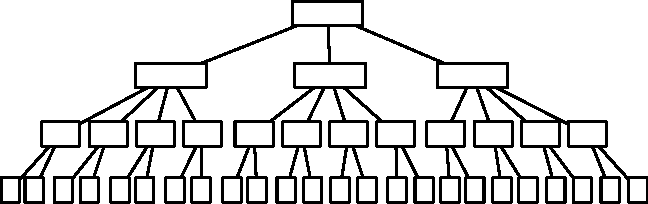
\includegraphics[width=\textwidth]{slike/komb_drevo.pdf}
   \end{center}
  \beforecaptionskip
  \caption{Kombinatorično drevo.}
  \label{fig:komb:drevo}
\end{figure}

\subsection{Permutacije}
\label{sec:komb:perm}
Razporeditve $n$ elementov v ravno vrsto so \textbf{permutacije} $n$ elementov. Število permutacij
$n$ elementov označimo s $P_n$.
\[ P_n = n\krat(n-1)\krat(n-2)\krat \,\cdots\, \krat 3 \krat 2 \krat 1 \]

Za namen računanja takih produktov definirajmo \textbf{fakulteto} ($n!$, beri $n$
fakulteta).
\[ n! = 1 \krat 2 \krat 3 \krat \,\cdots\, \krat (n-1) \krat n = \prod_{i=1}^ni \]
Dodatno definirajmo še $0! = 1$.

Število permutacije je tako enako
\[ P_n = n! \]

Permutacije so vse možne \textbf{bijektivne preslikave} množice same nase.

\subsection{Permutacije s ponavljanjem}
\label{sec:komb:ppon}
Permutacije $n$ elementov s ponavljanjem so vse možne razporeditve $n$ elementov v vrsto,
pri čemer dopuščamo \textbf{ponavljanje} elementov. 
\[ P_n^{k_1,k_2,\ldots,k_r} = \frac{n!}{k_1!k_2!\cdots k_r!} =
\frac{n!}{\displaystyle \prod_{i=1}^rk_i!} \qquad \sum_{i=1}^rk_i \le n \]

Izpeljava formule: Denimo, da imamo tri elemente, ki jih postavljamo v vrsto: $AB_1B_2$.
Njihove permutacije so: $AB_1B_2, AB_2B_1, B_1AB_2, B_1B_2A, B_2AB_1, B_2B_1A$.
Če $B$-jev sedaj ne razlikujemo med seboj, opazimo, da je vseh permutacij ravno dvakrat
preveč, ker lahko $B_1$ in $B_2$ permutiramo na $2! = 2$ načinov. Če bi imeli $k$ enakih
$B$-jev, bi imeli $k!$-krat preveč permutacij. Če bi imeli $r$
elementov, izmed katerih se $i$-it ponavlja $k_i$-krat, potem je vseh permutacij ravno 
$k_1!k_2! \cdots k_i! \cdots k_r!$ krat preveč, zato število vseh permutacij delimo s tem
produktom.

Primer: Koliko besed lahko sestavimo iz črk besede \texttt{MATEMATIKA}?
\[ n = P_{10}^{3,2,2} = \frac{10!}{3!2!2!} = 151200 \]

\subsection{Variacije}
\label{sec:komb:var}

\textbf{Variacije} reda $r$ iz $n$ elementov so vse možne razporeditve $r$ elementov v
vrsto, pri čemer elemente izbiramo iz množice z $n$ elementi.

\[ V_n^r = \frac{n!}{(n-r)!} \qquad r \le n \]

Izpeljava formule: Imejmo mesta v vrsti od 1 do $r$:
za prvo mesto izbiramo med $n$ elementi, za drugo med $n-1$ elementi, za $r$-to med
$n-(r-1)$ elementi. Torej je vseh možnosti po pravilu produkta enako
\[ n \krat (n-1) \krat (n-2) \krat \, \cdots \, \krat (n-r+1) \]
Pa recimo, da si to ful želimo zapisat s fakultetami in opazimo, da je produkt skoraj enak
$n!$, če bi le imel še člene $(n-r)!\krat(n-r-1)! \krat \, \cdots \, \krat 2!\krat
1!$. Pa jih dodamo, ampak da ohranimo vrednost izraza, moramo s tem tudi deliti. In to je
zapisano v zgornji formuli.

Variacije so vse možne \textbf{injektivne preslikave} iz množice z močjo $r$ v množico z močjo
$n$.

Primer: Na koliko načinov lahko postavimo 3 dekleta v vrsto pred tablo, če izbiramo med 12
dekleti v razredu.
\[ n = V_{12}^3 = \frac{12!}{9!} = 12\krat 11 \krat 10 = 1320 \]

\subsection{Variacije s ponavljanjem}
\label{sec:komb:varp}
Variacije reda $r$ iz $n$ elementov s ponavljanjem so vse možne razporeditve $r$ elementov
v vrsto, pri čemer elemente izbiramo iz množice z $n$ elementi in dopuščamo ponavljanje.

\[ ^{(p)}V_n^r = n^r \]

Izpeljava formule: Elemente postavljamo v vrsto z mesti od 1 do $r$. Za prvo mesto izbiramo
med $n$ elementi. Za drugo mesto prav tako izbiramo med $n$ elementi. O glej, za vsako
izmed $r$ mest izbiramo med $n$ elementi. Tako je po osnovnem izreku kombinatorike vseh
možnosti $\underbrace{n \krat n \krat n \krat \, \cdots \, \krat n}_{r} = n^r$.

Variacije s ponavljanjem so vse možne \textbf{preslikave} iz množice z močjo $r$ v množico z močjo
$n$.

\subsection{Kombinacije}
\label{sec:komb:komb}

Kombinacije reda $r$ iz $n$ elementov so vse \textbf{podmnožice} z močjo $r$ množice z močjo $n$.

\[ C_n^r = \frac{V_n^r}{r!} = \frac{n!}{(n-r)!\krat r!} \qquad r \le n\]

Izpeljava formule: Vseh možnih razporeditev $r$ elementov iz $n$ elementov je $V_n^r$.
Vendar smo pri tem upoštevali tudi vrstni red elementov. Ker pa delamo z množicami, vrstni
red ni pomemben in smo dobili, če smo izbirali $r$ elementov, ne le vse možne različne
elemente, temveč tudi na vse načine razporejene vse možne različne elemente. Načinov
razporeditve $r$ elementov je $r!$, in ravno tolikokrat preveč smo jih dobili, zato
število variacij delimo z $r!$.

Primer: V razredu je 30 dijakov. Koliko različnih skupin po 3 lahko oblikujejo?
\[ n = C_{30}^3 = \frac{30!}{27!\krat 3!} = 4060 \]

\subsection{Kombinacije s ponavljanjem}
\label{sec:komb:kombp}

Kombinacije s ponavljanjem reda $r$ iz $n$ elementov so vse podmnožice z močjo $r$ množice
z močjo $r$, pri čemer dopuščamo, da se elementi ponavljajo.
\[ ^{(p)}C_n^r = C_{n+r-1}^r \]

Primer: Na razpolago imamo 3 vrste čaja v vrečkah. Za pripravo vrča čaja
potrebujemo 7 vrečk. Koliko različnih mešanic čaja lahko pripravimo?
\[ n =\ ^{(p)}C_3^7 = C_9^7 = \frac{9!}{7!\krat 2!} = 36 \]

\subsection{Binomski koeficienti in binomski izrek}
\label{sec:komb:bin}

Definirajmo \textbf{binomski koeficient} oz. binomski simbol (simbol beremo $n$ nad $r$)
\[ \binom{n}{r} = C^r_n = \frac{n!}{(n-r)!r!} \]

Vrednost binomskega koeficienta je odgovor na vprašanje: ``Koliko je podmnožic z močjo $r$
množice z močjo $n$?''

\textbf{Osnovne vrednosti} binomskih simbolov: 
\[ \binom{n}{0} = 1 \qquad \binom{n}{1} = n \qquad \binom{n}{n} = 1 \]

Za binomske simbole veljata tudi dve lastnosti: simetričnost in aditivnost. \\
\textbf{Simetričnost:}
\[ \binom{n}{r} = \binom{n}{n-r} \]
Dokaz:
\begin{align*}
  \frac{n!}{(n-r)!r!} &= \frac{n!}{(n-(n-r))!(n-r)!} \\
  \frac{n!}{(n-r)!r!} &= \frac{n!}{r!(n-r)!}
\end{align*}
Simetričnost se vidi tudi takole: če ima množica s 100 elementi $k$ podmnožic s 75 elementi, ima
tudi $k$ podmnožic s 25 elementi, saj vsaki podmnožici s 75 elementi ustreza določena množica s 25
elementi.

\textbf{Aditivnost:}
\[ \binom{n}{r} + \binom{n}{r+1} = \binom{n+1}{r+1} \]
Dokaz:
\begin{align*}
  &\binom{n}{r} + \binom{n}{r+1} = \frac{n!}{(n-r)!r!} + \frac{n!}{(n-r-1)!(r+1)!} = \\
  &= \frac{n!}{r!(n-r-1)!}\left( \frac{1}{n-r} + \frac{1}{r+1} \right) =
  \frac{n!}{r!(n-r-1)!}\left( \frac{r+1+n-r}{(n-r)(r+1)} \right) = \\
  &= \frac{n!(n+1)}{r!(r+1)(n-r-1)!(n-r)} = \frac{(n+1)!}{(r+1)!(n-r)!} = \\
  &= \binom{n+1}{r+1}
\end{align*}

\subsubsection{Pascalov trikotnik}
\label{sec:komb:bin:pasc}
Pascalov trikotnik je trikotnik kjer so v vrsticah in stolpcih zapisani posamezni binomski koeficienti.

\begin{tabular}{rccccccccccc}
  $n=0$:&    &    &    &    &    &  $\binom{0}{0}$ \\\noalign{\smallskip\smallskip}
  $n=1$:&    &    &    &    &  $\binom{1}{0}$ &    &  $\binom{1}{1}$ \\\noalign{\smallskip\smallskip}
  $n=2$:&    &    &    &  $\binom{2}{0}$ &    &  $\binom{2}{1}$ &    &  $\binom{2}{2}$ \\\noalign{\smallskip\smallskip}
  $n=3$:&    &    &  $\binom{3}{0}$ &    &  $\binom{3}{1}$ &    &  $\binom{3}{2}$ &    & $\binom{3}{1}$ \\\noalign{\smallskip\smallskip}
  $n=4$:&    &  $\binom{4}{0}$ &    &  $\binom{4}{1}$ &    &  $\binom{4}{2}$ &    & $\binom{4}{3}$ &    & $\binom{4}{4}$ \\\noalign{\smallskip\smallskip}
  $n=5$:& $\binom{5}{0}$ &    &  $\binom{5}{1}$ &    & $\binom{5}{2}$ &    & $\binom{5}{3}$ &    & $\binom{5}{4}$ &    &  $\binom{5}{5}$\\\noalign{\smallskip\smallskip}
\end{tabular}


\begin{tabular}{rccccccccccccc}
$n=0$:&    &    &    &    &    &    &  1\\\noalign{\smallskip\smallskip}
$n=1$:&    &    &    &    &    &  1 &    &  1\\\noalign{\smallskip\smallskip}
$n=2$:&    &    &    &    &  1 &    &  2 &    &  1\\\noalign{\smallskip\smallskip}
$n=3$:&    &    &    &  1 &    &  3 &    &  3 &    &  1\\\noalign{\smallskip\smallskip}
$n=4$:&    &    &  1 &    &  4 &    &  6 &    &  4 &    &  1\\\noalign{\smallskip\smallskip}
$n=5$:&    &  1 &    &  5 &    & 10 &    & 10 &    &  5 &    &  1\\\noalign{\smallskip\smallskip}
$n=6$:&  1 &    &  6 &    & 15 &    & 20 &    & 15 &    &  6 &    &  1\\\noalign{\smallskip\smallskip}
\end{tabular}


Koeficienti ob levi in desni strani Pascalovega trikotnika so vedno enaki 1, ena izmed osnovnih
vrednosti binomskega simbola. Simetričnost binomskih koeficientov se kaže tudi v simetričnosti
Pascalovega trikotnika. Vsako novo vrstico (razen prvega in zadnjega koeficienta v vrstici) dobimo iz prejšnje
po pravilu aditivnosti: koeficienta levo in desno zgoraj od želenega se seštejeta ravno vanj. Tako
lahko precej enostavno zapišemo prvih nekaj vrstic Pascalovega trikotnika.

\subsubsection{Binomski izrek}
\label{sec:komb:bin:bin}
Binomski izrek je izrek, ki opisuje potenciranje \textbf{binoma}\footnote{Binom je druga beseda za
dvočlenik.} z naravnim številom ali 0.
\begin{gather*}
  (a+b)^n = \sum_{r=0}^n\binom{n}{r}a^{n-r}b^r = \\
  = \textstyle \binom{n}{0}a^nb^0 + \binom{n}{1}a^{n-1}b^1 + \binom{n}{2}a^{n-2}b^2 + \cdots +
  \binom{n}{n-2}a^2b^{n-2} + \binom{n}{n-1}a^1b^{n-1} + \binom{n}{n}a^0b^n
\end{gather*}

Pravimo, da razvijemo binom v \textbf{binomsko vrsto}. Splošni člen te binomske vrste je
\[ \binom{n}{r}a^{n-r}b^r \comment{To je $r+1$-ti člen!!, ker se začne z $r = 0$} \]

Razlaga formule:\\
Potencirajmo na primer $(a+b)^5 = (a+b)(a+b)(a+b)(a+b)(a+b)(a+b)$. Ko bi te oklepaje množili med
seboj, bi lahko iz vseh izbrali $a$ in bi dobili člen $a^5$. Seveda moramo množiti vsakega z vsakim,
in tako moramo tudi izbrati en $b$ in 4 $a$-je, da dobimo člen $a^4b$. Vendar lahko ta $b$ izberemo
na več različnih načinov, na točno $C^1_5$ načinov. Podobno izbiramo 2 $b$-ja in 3 $a$-je, da dobimo
člen $a^3b^2$ in to lahko izberemo na $\binom{5}{2}$ možnih načinov. Tako pridemo nazadnje do člena
$b^5$, kjer izberemo samo vse $b$-je, na en sam možen način.

Iz binomskega izreka tudi sledi, da je vsota posamezne vrstice v Pascalovem trikotniku enaka $2^n$.
\textbf{Število podmnožic} neke množice je prav tako enako $2^n$. Število podmnožic množice z močjo $n$ lahko
zapišemo kot število podmnožic z močjo 0 + število podmnožic z močjo $1 + \cdots + $ število
podmnožic z močjo $n$, ali drugače
\[ \binom{n}{0} + \binom{n}{1} + \cdots + \binom{n}{n-1} + \binom{n}{n} \comment{$n$-ta
vrstica Pascalovega trikotnika} \]
T\'{a}ko binomsko vrsto pa lahko dobimo le, če potenciramo binom $(1+1)^n$, kar pa je enako $2^n$. Duh.

\section{Verjetnostni račun}
\label{sec:verj}
Verjetnostni \textbf{poskus} je poskus, katerega rezultat je odvisen od naključja.
Osnovne rezultate verjetnostnega poskusa imenujemo \textbf{izidi} ali \textbf{elementarni
dogodki}. Označimo jih z $e_1, e_2, \dots, e_n$.

\textbf{Dogodek} je vsak pojav, ki se lahko zgodi pri poskusu. Dogodek lahko zapišemo kot
\textbf{množico elementarnih dogodkov}, ki so za ta dogodek ugodni.
\textbf{Univerzalna množica} je množica vseh elementarnih dogodkov. Njeno moč označimo z
$n$.

\textbf{Nemogoč dogodek} je dogodek, ki se pri poskusu ne more zgoditi. Predstavlja ga prazna
množica $\emptyset$.
\textbf{Gotov dogodek} je dogodek, ki se zgodi vedno. Predstavlja ga univerzalna množica
$\mathcal U$.

Množica vseh možnih dogodkov je potenčna množica množice $\mathcal U$. Vseh možnih
dogodkov je $|\mathcal P (\mathcal U)| = 2^n$.

Dogodka, ki se ne moreta zgoditi hkrati, se imenujeta \textbf{nezdružljiva} dogodka, dogodka, ki pa
se lahko zgodita hkrati, pa se imenujeta \textbf{združljiva} dogodka.

Primer:\\
Poskus: met poštene kocke\\
Elementarni dogodki: $\mathcal U = \{\text{pade 1}, \text{pade 2}, \text{pade 3},
\text{pade 4}, \text{pade 5}, \text{pade 6}\}$\\
Dogodek: $A = \{\text{pade praštevilo}\} = \{e_2, e_3, e_5\}$\\
Gotov dogodek: $B = \{\text{pade manj kot 9000}\} = \mathcal U$\\
Nemogoč dogodek: $C = \{\text{pade 13}\} = \{\}$ \\
Združljiva: $D = \{\text{pade sodo}\}$ in $A$. \\
Nezdružljiva: $E = \{e_1, e_3\}$ in $D$. \\

\subsection{Računanje z dogodki}
\label{sec:verj:racdog}
Dogodek $A'$ je \textbf{nasproten} dogodek dogodka A, ki se zgodi, če se ne zgodi $A$.
Če dogodek $A$ predstavimo z množico ugodnih izidov, dogodku $A'$ ustreza komplement
množice $A$.

\textbf{Vsota} ali unija dogodkov $A$ in $B$ je nov dogodek $A \cup B$ ($A+B$), ki se zgodi, če se
zgodi dogodek $A$ ali dogodek $B$.

\textbf{Produkt} ali presek dogodkov $A$ in $B$ je nov dogodek $A \cap B$ ($A\krat B$), ki se
zgodi, če se zgodita dogodka $A$ in $B$ hkrati. Če je produkt dogodkov enak nič, sta
dogodka nezdružljiva.

\textbf{Razlika} dogodkov $A$ in $B$ je nov dogodek $A - B$, ki se zgodi, če se zgodi dogodek $A$
in ne dogodek $B$.

Dogodek $A$ je način dogodka $B$, če se vedno, kadar se zgodi $A$, hkrati zgodi tudi $B$.
Če dogodka predstavimo z množicama ugodnih izidov, to pomeni, da je $A$ podmnožica množice
$B$.

\subsection{Klasična definicija verjetnosti}
\label{sec:verj:def}

Naj bo množica $\mathcal P(\mathcal U)$ množica vseh dogodkov pri poskusu. Verjetnost ($P$) je
funkcija, ki množico $\mathcal P (\mathcal U)$ preslika v množico realnih števil, če so
izpolnjeni sledeči aksiomi:
\begin{enumerate*}
  \item Verjetnost dogodka je vedno \textbf{večja ali enaka 0}.
  \item Verjetnost \textbf{gotovega} dogodka je enaka \textbf{1}. $P(\mathcal U) = 1$
    \label{enum:ver:aks:got}
  \item Če sta dogodka $A$ in $B$ \textbf{nezdružljiva} je verjetnost teh dveh dogodkov
    enaka \textbf{vsoti} verjetnosti posameznih dogodkov.
    \[ A \cap B = \emptyset \implies P(A \cup B) = P(A) + P(B) \] \label{enum:ver:aks:vsota}
\end{enumerate*}

\vspace{-5ex}
Naj bo pri poskusu možnih $n$ elementarnih dogodkov, ki so enako verjetni. Potem je
verjetnost vsakega od njih $\frac{1}{n}$. 
\[ P(e_i) = \frac{1}{n} \]

Dokaz:
\begin{align*}
  \mathcal U &=  e_1 \cup e_2 \cup \cdots \cup e_n \\
  P(\mathcal U) &= P(e_1 \cup e_2 \cup \cdots \cup e_n) \\
  1 &= P(e_1) + P(e_2) + \cdots + P(e_n) \comment{Po aksiomih \ref{enum:ver:aks:got} in
  \ref{enum:ver:aks:vsota}.} \\
  1 &= n\krat P(e_i) \comment{Ker so vsi enako verjetni.} \\
  P(e_i) &= \frac{1}{n}
\end{align*}

Naj bo za dogodek $A$ ugodnih $m$ \textbf{elementarnih} dogodkov, pri poskusu, pri katerem imamo
$n$ možnih enako verjetnih elementarnih dogodkov. Verjetnost dogodka $A$ je enaka
kvocientu med številom ugodnih elementarnih dogodkov in vseh elementarnih dogodkov.
\[ P(A) = \frac{m}{n} \]

Dokaz:
\begin{align*}
  A &= \{\underbrace{e_x, \ldots, e_y}_m\} \\
  P(A) &= P(\{\underbrace{e_x, \ldots, e_y}_m\}) \\
  P(A) &= \underbrace{P(e_x) + \cdots + P(e_y)}_m \\
  P(A) &= m \krat \frac{1}{n} \\
  P(A) &= \frac{m}{n}
\end{align*}

Obstaja tudi statistična definicija verjetnosti, pa še kakšna druga tudi. Po statistični
definiciji verjetnosti je verjetnost limita relativne frekvence, ko gre število poskusov v
neskončno. 

\subsection{Verjetnost nasprotnega dogodka}
\label{sec:verj:nasp}
Vsota verjetnosti dogodka in verjetnosti njemu nasprotnega dogodka je enaka 1.
\begin{gather*}
  A \cup A' = \mathcal U \\
  P(A \cup A') = P(\mathcal U) \\
  P(A) + P(A') = 1 \comment{$A$ in $A'$ sta nezdružljiva.} \\
  P(A) = 1 - P(A')  
\end{gather*}

\subsection{Verjetnost vsote združljivih dogodkov}
\label{sec:verj:zdruz}

Imejmo dogodka $A$ in $B$, ki naj bosta združljiva. Primer je prikazan na
sliki~\ref{fig:verj:zdruz}.
Število ugodnih elementarnih dogodkov za ta dogodek je tako enako:
\begin{gather*}
  m_{A\cup B} = m_A + m_B - m_{A\cap B} \\
  P(A \cup B) = \frac{m_A + m_B - m_{A\cap B}}{n} \\
  P(A \cup B) = \frac{m_A}{n} + \frac{m_B}{n} - \frac{m_{A\cap B}}{n} \\
  P(A \cup B) = P(A) + P(B) - P(A\cap B)
\end{gather*}

\begin{figure}[h]
  \begin{center}
    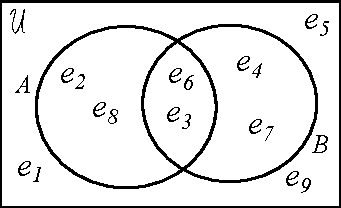
\includegraphics{slike/verjetnost_dogodki.pdf}
  \end{center}
  \beforecaptionskip
  \caption{Združljiva dogodka.}
  \label{fig:verj:zdruz}
\end{figure}

\subsection{Pogojna verjetnost}
\label{sec:verj:pog}

\textbf{Pogojna} verjetnost je verjetnost dogodka, pod \textbf{pogojem}, da se je neki drug dogodek že
zgodil. ($P(A|B)$, beri: verjetnost $A$, pri pogoju, da se je zgodil $B$.)

Pomagajmo si s sliko~\ref{fig:verj:zdruz}.
Če vemo da se je že zgodil dogodek $B$, potem je moč $B$ število vseh možnosti, ki jih
imamo, saj vemo, da se je $B$ že zgodil.
Število ugodnih možnosti pa je sedaj enako le še $m_{A\cap B}$, saj vemo, da so vse ugodne
možnosti elementi $A$-ja in $B$-ja. Verjetnost je tako enaka:
\[ P(A|B) = \frac{m_{A\cap B}}{m_B} = \frac{\frac{m_{A\cap B}}{n}}{\frac{m_B}{n}} =
\frac{P(A\cap B)}{P(B)} \]

\textbf{Verjetnost} dogodka $A$, pod \textbf{pogojem}, da se je zgodil dogodek $B$, je kvocient med
verjetnostjo produkta $A \cap B$ in verjetnostjo dogodka $B$.
\[ P(A|B) = \frac{P(A\cap B)}{P(B)} \]

Če zamenjamo črke dobimo:
\[ P(B|A) = \frac{P(A\cap B)}{P(A)} \]
in \textbf{verjetnost produkta} dogodkov je tako enaka:
\[ P(A\cap B) = P(A) \krat P(B|A) \]

Dogodka $A$ in $B$ sta neodvisna natanko takrat, kadar velja:
\[ P(A|B) = P(A) \text{ in } P(B|A) = P(B) \]
To pomeni, da izid dogodka $B$ nima nikakršnega vpliva na možne izide dogodka $A$, in
obratno.

Verjetnost produkta \textbf{neodvisnih} dogodkov je enaka:
\[ P(A \cap B) = P(A)\krat P(B) \]

\subsection{Bernoullijevo zaporedje}
\label{sec:ver:bern}

Zaporedje \textbf{neodvisnih} poskusov je \textbf{Bernoullijevo zaporedje}, če se lahko v vsaki ponovitvi
poskusa zgodi samo dogodek $A$ z verjetnostjo $p$ ali njegov nasprotni dogodek.
\[ P(A) = p \qquad \quad P(A') = 1-p \]
Verjetnost, da se nek dogodek z verjetnostjo $p$ v $n$ ponovitvah poskusa zgodi natanko
$k$-krat, je enaka:
\[ P(n, p, k) = \binom{n}{k}p^k(1-p)^{n-k} \]

Pojasnijo formule:\\
Za lažjo obravnavo denimo, da nas zanima kolikšna je verjetnost, da se najprej zgodi
$k$ dogodkov $A$ in nato $n-k$ dogodkov $A'$.
\begin{gather*}
  P(\underbrace{A \cap A \cap \cdots \cap A}_k \cap \underbrace{A' \cap A' \cap \cdots
  \cap A'}_{n-k}) = \comment{Neodvisni dogodki.}\\
  = \underbrace{P(A)\krat P(A) \krat \, \cdots \, \krat P(A)}_k \krat
  \underbrace{P(A')\krat P(A')\krat \, \cdots \, \krat P(A')}_{n-k} = \\
  = (P(A))^k \krat (P(A'))^{n-k} = p^k(1-p)^{n-k}
\end{gather*}
Sedaj pa se vrnimo na osnovni problem. Ne zanima nas vrstni red v katerem se je zgodilo
$k$ dogodkov $A$, zanima nas le verjetnost, da se jih je zgodilo $k$. Na koliko 
različnih načinov pa se lahko zgodi $k$ dogodkov $A$ v $n$ poskusih? Na $C^k_n =
\binom{n}{k}$, torej je verjetnost, da se zgodi dogodek $A$, ravno $\binom{n}{k}$-krat večja.

%%%%%%%%%%%%%%%%%%%%%%%%%%

\pagebreak
\listoffigures
%\pagebreak
%\printindex

\end{document}
% pazi kje je kazalo slik !!!
% vim: spell spelllang=sl
